\documentclass[twoside]{book}

% Packages required by doxygen
\usepackage{fixltx2e}
\usepackage{calc}
\usepackage{doxygen}
\usepackage[export]{adjustbox} % also loads graphicx
\usepackage{graphicx}
\usepackage[utf8]{inputenc}
\usepackage{makeidx}
\usepackage{multicol}
\usepackage{multirow}
\PassOptionsToPackage{warn}{textcomp}
\usepackage{textcomp}
\usepackage[nointegrals]{wasysym}
\usepackage[table]{xcolor}

% Font selection
\usepackage[T1]{fontenc}
\usepackage[scaled=.90]{helvet}
\usepackage{courier}
\usepackage{amssymb}
\usepackage{sectsty}
\renewcommand{\familydefault}{\sfdefault}
\allsectionsfont{%
  \fontseries{bc}\selectfont%
  \color{darkgray}%
}
\renewcommand{\DoxyLabelFont}{%
  \fontseries{bc}\selectfont%
  \color{darkgray}%
}
\newcommand{\+}{\discretionary{\mbox{\scriptsize$\hookleftarrow$}}{}{}}

% Page & text layout
\usepackage{geometry}
\geometry{%
  a4paper,%
  top=2.5cm,%
  bottom=2.5cm,%
  left=2.5cm,%
  right=2.5cm%
}
\tolerance=750
\hfuzz=15pt
\hbadness=750
\setlength{\emergencystretch}{15pt}
\setlength{\parindent}{0cm}
\setlength{\parskip}{3ex plus 2ex minus 2ex}
\makeatletter
\renewcommand{\paragraph}{%
  \@startsection{paragraph}{4}{0ex}{-1.0ex}{1.0ex}{%
    \normalfont\normalsize\bfseries\SS@parafont%
  }%
}
\renewcommand{\subparagraph}{%
  \@startsection{subparagraph}{5}{0ex}{-1.0ex}{1.0ex}{%
    \normalfont\normalsize\bfseries\SS@subparafont%
  }%
}
\makeatother

% Headers & footers
\usepackage{fancyhdr}
\pagestyle{fancyplain}
\fancyhead[LE]{\fancyplain{}{\bfseries\thepage}}
\fancyhead[CE]{\fancyplain{}{}}
\fancyhead[RE]{\fancyplain{}{\bfseries\leftmark}}
\fancyhead[LO]{\fancyplain{}{\bfseries\rightmark}}
\fancyhead[CO]{\fancyplain{}{}}
\fancyhead[RO]{\fancyplain{}{\bfseries\thepage}}
\fancyfoot[LE]{\fancyplain{}{}}
\fancyfoot[CE]{\fancyplain{}{}}
\fancyfoot[RE]{\fancyplain{}{\bfseries\scriptsize Generated by Doxygen }}
\fancyfoot[LO]{\fancyplain{}{\bfseries\scriptsize Generated by Doxygen }}
\fancyfoot[CO]{\fancyplain{}{}}
\fancyfoot[RO]{\fancyplain{}{}}
\renewcommand{\footrulewidth}{0.4pt}
\renewcommand{\chaptermark}[1]{%
  \markboth{#1}{}%
}
\renewcommand{\sectionmark}[1]{%
  \markright{\thesection\ #1}%
}

% Indices & bibliography
\usepackage{natbib}
\usepackage[titles]{tocloft}
\setcounter{tocdepth}{3}
\setcounter{secnumdepth}{5}
\makeindex

% Hyperlinks (required, but should be loaded last)
\usepackage{ifpdf}
\ifpdf
  \usepackage[pdftex,pagebackref=true]{hyperref}
\else
  \usepackage[ps2pdf,pagebackref=true]{hyperref}
\fi
\hypersetup{%
  colorlinks=true,%
  linkcolor=blue,%
  citecolor=blue,%
  unicode%
}

% Custom commands
\newcommand{\clearemptydoublepage}{%
  \newpage{\pagestyle{empty}\cleardoublepage}%
}

\usepackage{caption}
\captionsetup{labelsep=space,justification=centering,font={bf},singlelinecheck=off,skip=4pt,position=top}

%===== C O N T E N T S =====

\begin{document}

% Titlepage & ToC
\hypersetup{pageanchor=false,
             bookmarksnumbered=true,
             pdfencoding=unicode
            }
\pagenumbering{alph}
\begin{titlepage}
\vspace*{7cm}
\begin{center}%
{\Large My Project }\\
\vspace*{1cm}
{\large Generated by Doxygen 1.8.12}\\
\end{center}
\end{titlepage}
\clearemptydoublepage
\pagenumbering{roman}
\tableofcontents
\clearemptydoublepage
\pagenumbering{arabic}
\hypersetup{pageanchor=true}

%--- Begin generated contents ---
\chapter{Hierarchical Index}
\section{Class Hierarchy}
This inheritance list is sorted roughly, but not completely, alphabetically\+:\begin{DoxyCompactList}
\item \contentsline{section}{Builder\+Subsistema\+Desenvolvedor\+Teste}{\pageref{class_builder_subsistema_desenvolvedor_teste}}{}
\item \contentsline{section}{Builder\+Subsistema\+Gerente\+Projeto\+Teste}{\pageref{class_builder_subsistema_gerente_projeto_teste}}{}
\item \contentsline{section}{Builder\+Subsistema\+Gerente\+Sistema\+Teste}{\pageref{class_builder_subsistema_gerente_sistema_teste}}{}
\item \contentsline{section}{Builder\+Subsistema\+Projeto\+Teste}{\pageref{class_builder_subsistema_projeto_teste}}{}
\item \contentsline{section}{Cntr\+I\+U\+Gerente\+Sistema\+:\+:Cntr\+Edicao}{\pageref{class_cntr_i_u_gerente_sistema_1_1_cntr_edicao}}{}
\item \contentsline{section}{C\+Cntr\+I\+U\+Gerente\+Sistema\+:\+:Cntr\+Edicao}{\pageref{class_c_cntr_i_u_gerente_sistema_1_1_cntr_edicao}}{}
\item \contentsline{section}{Cntr\+I\+U\+Gerente\+Projeto\+:\+:Cntr\+Edicao}{\pageref{class_cntr_i_u_gerente_projeto_1_1_cntr_edicao}}{}
\item \contentsline{section}{Cntr\+I\+U\+Gerente\+Projeto\+:\+:Cntr\+Inclusao}{\pageref{class_cntr_i_u_gerente_projeto_1_1_cntr_inclusao}}{}
\item \contentsline{section}{Cntr\+I\+U\+Gerente\+Sistema\+:\+:Cntr\+Inclusao}{\pageref{class_cntr_i_u_gerente_sistema_1_1_cntr_inclusao}}{}
\item \contentsline{section}{Cntr\+I\+U\+Gerente\+Sistema\+:\+:Cntr\+Pesquisa}{\pageref{class_cntr_i_u_gerente_sistema_1_1_cntr_pesquisa}}{}
\item \contentsline{section}{Cntr\+I\+U\+Gerente\+Projeto\+:\+:Cntr\+Pesquisa}{\pageref{class_cntr_i_u_gerente_projeto_1_1_cntr_pesquisa}}{}
\item \contentsline{section}{Cntr\+I\+U\+Gerente\+Projeto\+:\+:Cntr\+Remocao}{\pageref{class_cntr_i_u_gerente_projeto_1_1_cntr_remocao}}{}
\item \contentsline{section}{Cntr\+I\+U\+Gerente\+Sistema\+:\+:Cntr\+Remocao}{\pageref{class_cntr_i_u_gerente_sistema_1_1_cntr_remocao}}{}
\item \contentsline{section}{Codigo\+Projeto}{\pageref{class_codigo_projeto}}{}
\item \contentsline{section}{Comando\+Banco\+Dados}{\pageref{class_comando_banco_dados}}{}
\begin{DoxyCompactList}
\item \contentsline{section}{Comando\+Editar\+Desenvolvedor}{\pageref{class_comando_editar_desenvolvedor}}{}
\item \contentsline{section}{Comando\+Editar\+Gerente\+Projeto}{\pageref{class_comando_editar_gerente_projeto}}{}
\item \contentsline{section}{Comando\+Editar\+Gerente\+Sistema}{\pageref{class_comando_editar_gerente_sistema}}{}
\item \contentsline{section}{Comando\+Editar\+Projeto}{\pageref{class_comando_editar_projeto}}{}
\item \contentsline{section}{Comando\+Incluir\+Desenvolvedor}{\pageref{class_comando_incluir_desenvolvedor}}{}
\item \contentsline{section}{Comando\+Incluir\+Gerente}{\pageref{class_comando_incluir_gerente}}{}
\item \contentsline{section}{Comando\+Incluir\+Gerente\+Projeto}{\pageref{class_comando_incluir_gerente_projeto}}{}
\item \contentsline{section}{Comando\+Incluir\+Gerente\+Sistema}{\pageref{class_comando_incluir_gerente_sistema}}{}
\item \contentsline{section}{Comando\+Incluir\+Projeto}{\pageref{class_comando_incluir_projeto}}{}
\item \contentsline{section}{Comando\+Recuperar\+Desenvolvedor}{\pageref{class_comando_recuperar_desenvolvedor}}{}
\item \contentsline{section}{Comando\+Recuperar\+Gerente\+Projeto}{\pageref{class_comando_recuperar_gerente_projeto}}{}
\item \contentsline{section}{Comando\+Recuperar\+Gerente\+Sistema}{\pageref{class_comando_recuperar_gerente_sistema}}{}
\item \contentsline{section}{Comando\+Recuperar\+Projeto}{\pageref{class_comando_recuperar_projeto}}{}
\item \contentsline{section}{Comando\+Remover\+Desenvolvedor}{\pageref{class_comando_remover_desenvolvedor}}{}
\item \contentsline{section}{Comando\+Remover\+Gerente\+Projeto}{\pageref{class_comando_remover_gerente_projeto}}{}
\item \contentsline{section}{Comando\+Remover\+Gerente\+Sistema}{\pageref{class_comando_remover_gerente_sistema}}{}
\item \contentsline{section}{Comando\+Remover\+Projeto}{\pageref{class_comando_remover_projeto}}{}
\end{DoxyCompactList}
\item \contentsline{section}{Comando\+Editar\+Gerente}{\pageref{class_comando_editar_gerente}}{}
\item \contentsline{section}{Comando\+Recuperar\+Gerente}{\pageref{class_comando_recuperar_gerente}}{}
\item \contentsline{section}{Comando\+Recuperar\+Sistema}{\pageref{class_comando_recuperar_sistema}}{}
\item \contentsline{section}{Comando\+Remover\+Gerente}{\pageref{class_comando_remover_gerente}}{}
\item \contentsline{section}{Custo}{\pageref{class_custo}}{}
\item \contentsline{section}{Data}{\pageref{class_data}}{}
\item \contentsline{section}{Email}{\pageref{class_email}}{}
\item \contentsline{section}{Estado\+Projeto}{\pageref{class_estado_projeto}}{}
\item \contentsline{section}{Fase}{\pageref{class_fase}}{}
\item \contentsline{section}{Fase\+Projeto}{\pageref{class_fase_projeto}}{}
\item \contentsline{section}{Funcao}{\pageref{class_funcao}}{}
\item \contentsline{section}{I\+L\+N\+Autenticacao}{\pageref{class_i_l_n_autenticacao}}{}
\begin{DoxyCompactList}
\item \contentsline{section}{Stub\+L\+N\+Autenticacao}{\pageref{class_stub_l_n_autenticacao}}{}
\end{DoxyCompactList}
\item \contentsline{section}{I\+L\+N\+Desenvolvedor}{\pageref{class_i_l_n_desenvolvedor}}{}
\begin{DoxyCompactList}
\item \contentsline{section}{Stub\+L\+N\+Desenvolvedor}{\pageref{class_stub_l_n_desenvolvedor}}{}
\end{DoxyCompactList}
\item \contentsline{section}{I\+L\+N\+Gerente\+Projeto}{\pageref{class_i_l_n_gerente_projeto}}{}
\begin{DoxyCompactList}
\item \contentsline{section}{Stub\+L\+N\+Gerente\+Projeto}{\pageref{class_stub_l_n_gerente_projeto}}{}
\end{DoxyCompactList}
\item \contentsline{section}{I\+L\+N\+Gerente\+Sistema}{\pageref{class_i_l_n_gerente_sistema}}{}
\begin{DoxyCompactList}
\item \contentsline{section}{Stub\+L\+N\+Gerente\+Sistema}{\pageref{class_stub_l_n_gerente_sistema}}{}
\end{DoxyCompactList}
\item \contentsline{section}{I\+L\+N\+Projeto}{\pageref{class_i_l_n_projeto}}{}
\begin{DoxyCompactList}
\item \contentsline{section}{Stub\+L\+N\+Projeto}{\pageref{class_stub_l_n_projeto}}{}
\end{DoxyCompactList}
\item \contentsline{section}{I\+Persistencia}{\pageref{class_i_persistencia}}{}
\begin{DoxyCompactList}
\item \contentsline{section}{Stub\+Persistencia}{\pageref{class_stub_persistencia}}{}
\end{DoxyCompactList}
\item \contentsline{section}{I\+U\+Autenticacao}{\pageref{class_i_u_autenticacao}}{}
\begin{DoxyCompactList}
\item \contentsline{section}{Cntr\+I\+U\+Autenticacao}{\pageref{class_cntr_i_u_autenticacao}}{}
\end{DoxyCompactList}
\item \contentsline{section}{I\+U\+Desenvolvedor}{\pageref{class_i_u_desenvolvedor}}{}
\begin{DoxyCompactList}
\item \contentsline{section}{Cntr\+I\+U\+Desenvolvedor}{\pageref{class_cntr_i_u_desenvolvedor}}{}
\end{DoxyCompactList}
\item \contentsline{section}{I\+U\+Gerente\+Projeto}{\pageref{class_i_u_gerente_projeto}}{}
\begin{DoxyCompactList}
\item \contentsline{section}{Cntr\+I\+U\+Gerente\+Projeto}{\pageref{class_cntr_i_u_gerente_projeto}}{}
\end{DoxyCompactList}
\item \contentsline{section}{I\+U\+Gerente\+Sistema}{\pageref{class_i_u_gerente_sistema}}{}
\begin{DoxyCompactList}
\item \contentsline{section}{Cntr\+I\+U\+Gerente\+Sistema}{\pageref{class_cntr_i_u_gerente_sistema}}{}
\end{DoxyCompactList}
\item \contentsline{section}{I\+U\+Projeto}{\pageref{class_i_u_projeto}}{}
\begin{DoxyCompactList}
\item \contentsline{section}{Cntr\+I\+U\+Projeto}{\pageref{class_cntr_i_u_projeto}}{}
\end{DoxyCompactList}
\item \contentsline{section}{Matricula}{\pageref{class_matricula}}{}
\item \contentsline{section}{Nome}{\pageref{class_nome}}{}
\item \contentsline{section}{Projeto}{\pageref{class_projeto}}{}
\item \contentsline{section}{Resultado}{\pageref{class_resultado}}{}
\begin{DoxyCompactList}
\item \contentsline{section}{Resultado\+Autenticacao}{\pageref{class_resultado_autenticacao}}{}
\item \contentsline{section}{Resultado\+Desenvolvedor}{\pageref{class_resultado_desenvolvedor}}{}
\item \contentsline{section}{Resultado\+Gerente\+Projeto}{\pageref{class_resultado_gerente_projeto}}{}
\item \contentsline{section}{Resultado\+Gerente\+Sistema}{\pageref{class_resultado_gerente_sistema}}{}
\item \contentsline{section}{Resultado\+Projeto}{\pageref{class_resultado_projeto}}{}
\end{DoxyCompactList}
\item \contentsline{section}{Senha}{\pageref{class_senha}}{}
\item \contentsline{section}{Stub\+L\+N\+A\+Gerente}{\pageref{class_stub_l_n_a_gerente}}{}
\item \contentsline{section}{Stub\+L\+N\+Gerente}{\pageref{class_stub_l_n_gerente}}{}
\item \contentsline{section}{Telefone}{\pageref{class_telefone}}{}
\item \contentsline{section}{T\+U\+Codigo\+Projeto}{\pageref{class_t_u_codigo_projeto}}{}
\item \contentsline{section}{T\+U\+Custo}{\pageref{class_t_u_custo}}{}
\item \contentsline{section}{T\+U\+Data}{\pageref{class_t_u_data}}{}
\item \contentsline{section}{T\+U\+Email}{\pageref{class_t_u_email}}{}
\item \contentsline{section}{T\+U\+Estado\+Projeto}{\pageref{class_t_u_estado_projeto}}{}
\item \contentsline{section}{T\+U\+Fase}{\pageref{class_t_u_fase}}{}
\item \contentsline{section}{T\+U\+Funcao}{\pageref{class_t_u_funcao}}{}
\item \contentsline{section}{T\+U\+Matricula}{\pageref{class_t_u_matricula}}{}
\item \contentsline{section}{T\+U\+Nome}{\pageref{class_t_u_nome}}{}
\item \contentsline{section}{T\+U\+Senha}{\pageref{class_t_u_senha}}{}
\item \contentsline{section}{T\+U\+Telefone}{\pageref{class_t_u_telefone}}{}
\item \contentsline{section}{Usuario}{\pageref{class_usuario}}{}
\begin{DoxyCompactList}
\item \contentsline{section}{Desenvolvedor}{\pageref{class_desenvolvedor}}{}
\item \contentsline{section}{Gerente\+Projeto}{\pageref{class_gerente_projeto}}{}
\item \contentsline{section}{Gerente\+Sistema}{\pageref{class_gerente_sistema}}{}
\end{DoxyCompactList}
\end{DoxyCompactList}

\chapter{Class Index}
\section{Class List}
Here are the classes, structs, unions and interfaces with brief descriptions\+:\begin{DoxyCompactList}
\item\contentsline{section}{\hyperlink{class_builder_subsistema_desenvolvedor_teste}{Builder\+Subsistema\+Desenvolvedor\+Teste} \\*Classe respons�vel por testar o construtor de \hyperlink{class_desenvolvedor}{Desenvolvedor} na interface }{\pageref{class_builder_subsistema_desenvolvedor_teste}}{}
\item\contentsline{section}{\hyperlink{class_builder_subsistema_gerente_projeto_teste}{Builder\+Subsistema\+Gerente\+Projeto\+Teste} \\*Classe respons�vel por testar o construtor de Gerente de \hyperlink{class_projeto}{Projeto} na interface }{\pageref{class_builder_subsistema_gerente_projeto_teste}}{}
\item\contentsline{section}{\hyperlink{class_builder_subsistema_gerente_sistema_teste}{Builder\+Subsistema\+Gerente\+Sistema\+Teste} \\*Classe respons�vel por testar o construtor de Gerente de Sistema na interface }{\pageref{class_builder_subsistema_gerente_sistema_teste}}{}
\item\contentsline{section}{\hyperlink{class_builder_subsistema_projeto_teste}{Builder\+Subsistema\+Projeto\+Teste} \\*Classe respons�vel por testar o construtor de \hyperlink{class_projeto}{Projeto} na interface }{\pageref{class_builder_subsistema_projeto_teste}}{}
\item\contentsline{section}{\hyperlink{class_cntr_i_u_gerente_sistema_1_1_cntr_edicao}{Cntr\+I\+U\+Gerente\+Sistema\+::\+Cntr\+Edicao} }{\pageref{class_cntr_i_u_gerente_sistema_1_1_cntr_edicao}}{}
\item\contentsline{section}{\hyperlink{class_c_cntr_i_u_gerente_sistema_1_1_cntr_edicao}{C\+Cntr\+I\+U\+Gerente\+Sistema\+::\+Cntr\+Edicao} \\*Classe interna respons�vel pela edi��o do gerente de sistema na interface l�gica de neg�cio }{\pageref{class_c_cntr_i_u_gerente_sistema_1_1_cntr_edicao}}{}
\item\contentsline{section}{\hyperlink{class_cntr_i_u_gerente_projeto_1_1_cntr_edicao}{Cntr\+I\+U\+Gerente\+Projeto\+::\+Cntr\+Edicao} \\*Classe interna respons�vel pela edi��o do gerente de projeto na interface l�gica de neg�cio }{\pageref{class_cntr_i_u_gerente_projeto_1_1_cntr_edicao}}{}
\item\contentsline{section}{\hyperlink{class_cntr_i_u_gerente_projeto_1_1_cntr_inclusao}{Cntr\+I\+U\+Gerente\+Projeto\+::\+Cntr\+Inclusao} \\*Classe interna respons�vel pela inclus�o do gerente de projeto na interface l�gica de neg�cio }{\pageref{class_cntr_i_u_gerente_projeto_1_1_cntr_inclusao}}{}
\item\contentsline{section}{\hyperlink{class_cntr_i_u_gerente_sistema_1_1_cntr_inclusao}{Cntr\+I\+U\+Gerente\+Sistema\+::\+Cntr\+Inclusao} \\*Classe interna respons�vel pela inclus�o do gerente de sistema na interface l�gica de neg�cio }{\pageref{class_cntr_i_u_gerente_sistema_1_1_cntr_inclusao}}{}
\item\contentsline{section}{\hyperlink{class_cntr_i_u_autenticacao}{Cntr\+I\+U\+Autenticacao} \\*Classe respons�vel por autentica��o na interface }{\pageref{class_cntr_i_u_autenticacao}}{}
\item\contentsline{section}{\hyperlink{class_cntr_i_u_desenvolvedor}{Cntr\+I\+U\+Desenvolvedor} \\*Classe respons�vel pelo controle do desenvolvedor na interface }{\pageref{class_cntr_i_u_desenvolvedor}}{}
\item\contentsline{section}{\hyperlink{class_cntr_i_u_gerente_projeto}{Cntr\+I\+U\+Gerente\+Projeto} \\*Classe respons�vel pelo controle do gerente de projeto na interface }{\pageref{class_cntr_i_u_gerente_projeto}}{}
\item\contentsline{section}{\hyperlink{class_cntr_i_u_gerente_sistema}{Cntr\+I\+U\+Gerente\+Sistema} \\*Classe respons�vel pelo controle do gerente de sistema na interface }{\pageref{class_cntr_i_u_gerente_sistema}}{}
\item\contentsline{section}{\hyperlink{class_cntr_i_u_projeto}{Cntr\+I\+U\+Projeto} \\*Classe respons�vel pelo controle do projeto na interface }{\pageref{class_cntr_i_u_projeto}}{}
\item\contentsline{section}{\hyperlink{class_cntr_i_u_gerente_sistema_1_1_cntr_pesquisa}{Cntr\+I\+U\+Gerente\+Sistema\+::\+Cntr\+Pesquisa} \\*Classe interna respons�vel pela pesquisa do gerente de sistema na interface l�gica de neg�cio }{\pageref{class_cntr_i_u_gerente_sistema_1_1_cntr_pesquisa}}{}
\item\contentsline{section}{\hyperlink{class_cntr_i_u_gerente_projeto_1_1_cntr_pesquisa}{Cntr\+I\+U\+Gerente\+Projeto\+::\+Cntr\+Pesquisa} \\*Classe interna respons�vel pela pesquisa do gerente de projeto na interface l�gica de neg�cio }{\pageref{class_cntr_i_u_gerente_projeto_1_1_cntr_pesquisa}}{}
\item\contentsline{section}{\hyperlink{class_cntr_i_u_gerente_projeto_1_1_cntr_remocao}{Cntr\+I\+U\+Gerente\+Projeto\+::\+Cntr\+Remocao} \\*Classe interna respons�vel pela remo��o do gerente de projeto na interface l�gica de neg�cio }{\pageref{class_cntr_i_u_gerente_projeto_1_1_cntr_remocao}}{}
\item\contentsline{section}{\hyperlink{class_cntr_i_u_gerente_sistema_1_1_cntr_remocao}{Cntr\+I\+U\+Gerente\+Sistema\+::\+Cntr\+Remocao} \\*Classe interna respons�vel pela remo�ao do gerente de sistema na interface l�gica de neg�cio }{\pageref{class_cntr_i_u_gerente_sistema_1_1_cntr_remocao}}{}
\item\contentsline{section}{\hyperlink{class_codigo_projeto}{Codigo\+Projeto} \\*Classe que cont�m os principais m�todos do codigo do projeto do dominio }{\pageref{class_codigo_projeto}}{}
\item\contentsline{section}{\hyperlink{class_comando_banco_dados}{Comando\+Banco\+Dados} \\*Classe que contém os principais métodos dos comandos do banco de dados }{\pageref{class_comando_banco_dados}}{}
\item\contentsline{section}{\hyperlink{class_comando_editar_desenvolvedor}{Comando\+Editar\+Desenvolvedor} \\*Classe responsável por\+: Editar desenvolvedor }{\pageref{class_comando_editar_desenvolvedor}}{}
\item\contentsline{section}{\hyperlink{class_comando_editar_gerente}{Comando\+Editar\+Gerente} }{\pageref{class_comando_editar_gerente}}{}
\item\contentsline{section}{\hyperlink{class_comando_editar_gerente_projeto}{Comando\+Editar\+Gerente\+Projeto} \\*Classe responsável por\+: Editar Gerente de projeto }{\pageref{class_comando_editar_gerente_projeto}}{}
\item\contentsline{section}{\hyperlink{class_comando_editar_gerente_sistema}{Comando\+Editar\+Gerente\+Sistema} \\*Classe responsável por\+: Editar Gerente de sistema }{\pageref{class_comando_editar_gerente_sistema}}{}
\item\contentsline{section}{\hyperlink{class_comando_editar_projeto}{Comando\+Editar\+Projeto} \\*Classe responsável por\+: Editar projeto }{\pageref{class_comando_editar_projeto}}{}
\item\contentsline{section}{\hyperlink{class_comando_incluir_desenvolvedor}{Comando\+Incluir\+Desenvolvedor} \\*Classe responsável por\+: Incluir desenvolvedor }{\pageref{class_comando_incluir_desenvolvedor}}{}
\item\contentsline{section}{\hyperlink{class_comando_incluir_gerente}{Comando\+Incluir\+Gerente} \\*Classe responsável por\+: Incluir Gerente de projeto }{\pageref{class_comando_incluir_gerente}}{}
\item\contentsline{section}{\hyperlink{class_comando_incluir_gerente_projeto}{Comando\+Incluir\+Gerente\+Projeto} \\*Classe responsável por\+: Incluir Gerente de projeto }{\pageref{class_comando_incluir_gerente_projeto}}{}
\item\contentsline{section}{\hyperlink{class_comando_incluir_gerente_sistema}{Comando\+Incluir\+Gerente\+Sistema} \\*Classe responsável por\+: Incluir Gerente de sistema }{\pageref{class_comando_incluir_gerente_sistema}}{}
\item\contentsline{section}{\hyperlink{class_comando_incluir_projeto}{Comando\+Incluir\+Projeto} \\*Classe responsável por\+: Incluir projeto }{\pageref{class_comando_incluir_projeto}}{}
\item\contentsline{section}{\hyperlink{class_comando_recuperar_desenvolvedor}{Comando\+Recuperar\+Desenvolvedor} \\*Classe responsável por\+: Recuperar desenvolvedor }{\pageref{class_comando_recuperar_desenvolvedor}}{}
\item\contentsline{section}{\hyperlink{class_comando_recuperar_gerente}{Comando\+Recuperar\+Gerente} }{\pageref{class_comando_recuperar_gerente}}{}
\item\contentsline{section}{\hyperlink{class_comando_recuperar_gerente_projeto}{Comando\+Recuperar\+Gerente\+Projeto} \\*Classe responsável por\+: Recuperar Gerente de projeto }{\pageref{class_comando_recuperar_gerente_projeto}}{}
\item\contentsline{section}{\hyperlink{class_comando_recuperar_gerente_sistema}{Comando\+Recuperar\+Gerente\+Sistema} }{\pageref{class_comando_recuperar_gerente_sistema}}{}
\item\contentsline{section}{\hyperlink{class_comando_recuperar_projeto}{Comando\+Recuperar\+Projeto} \\*Classe responsável por\+: Recuperar projeto }{\pageref{class_comando_recuperar_projeto}}{}
\item\contentsline{section}{\hyperlink{class_comando_recuperar_sistema}{Comando\+Recuperar\+Sistema} \\*Classe responsável por\+: Recuperar Gerente de Sistema }{\pageref{class_comando_recuperar_sistema}}{}
\item\contentsline{section}{\hyperlink{class_comando_remover_desenvolvedor}{Comando\+Remover\+Desenvolvedor} \\*Classe responsável por\+: Remover desenvolvedor }{\pageref{class_comando_remover_desenvolvedor}}{}
\item\contentsline{section}{\hyperlink{class_comando_remover_gerente}{Comando\+Remover\+Gerente} }{\pageref{class_comando_remover_gerente}}{}
\item\contentsline{section}{\hyperlink{class_comando_remover_gerente_projeto}{Comando\+Remover\+Gerente\+Projeto} \\*Classe responsável por\+: Remover Gerente de projeto }{\pageref{class_comando_remover_gerente_projeto}}{}
\item\contentsline{section}{\hyperlink{class_comando_remover_gerente_sistema}{Comando\+Remover\+Gerente\+Sistema} \\*Classe responsável por\+: Remover Gerente de sistema }{\pageref{class_comando_remover_gerente_sistema}}{}
\item\contentsline{section}{\hyperlink{class_comando_remover_projeto}{Comando\+Remover\+Projeto} \\*Classe responsável por\+: Remover projeto }{\pageref{class_comando_remover_projeto}}{}
\item\contentsline{section}{\hyperlink{class_custo}{Custo} \\*Classe que cont�m os principais m�todos do custo do dominio }{\pageref{class_custo}}{}
\item\contentsline{section}{\hyperlink{class_data}{Data} \\*Classe que cont�m os principais m�todos da data do dominio }{\pageref{class_data}}{}
\item\contentsline{section}{\hyperlink{class_desenvolvedor}{Desenvolvedor} \\*Classe que cont�m os principais m�todos da entidade de desenvolvedor }{\pageref{class_desenvolvedor}}{}
\item\contentsline{section}{\hyperlink{class_email}{Email} \\*Classe que cont�m os principais m�todos do email do dominio }{\pageref{class_email}}{}
\item\contentsline{section}{\hyperlink{class_estado_projeto}{Estado\+Projeto} \\*Classe que cont�m os principais m�todos do Estado do \hyperlink{class_projeto}{Projeto} do dominio }{\pageref{class_estado_projeto}}{}
\item\contentsline{section}{\hyperlink{class_fase}{Fase} \\*Classe que cont�m os principais m�todos da fase do dominio }{\pageref{class_fase}}{}
\item\contentsline{section}{\hyperlink{class_fase_projeto}{Fase\+Projeto} \\*Classe que cont�m os principais m�todos da entidade de fase de projeto }{\pageref{class_fase_projeto}}{}
\item\contentsline{section}{\hyperlink{class_funcao}{Funcao} \\*Classe que cont�m os principais m�todos da fun��o do dominio }{\pageref{class_funcao}}{}
\item\contentsline{section}{\hyperlink{class_gerente_projeto}{Gerente\+Projeto} \\*Classe que cont�m os principais m�todos da entidade de gerente de projeto }{\pageref{class_gerente_projeto}}{}
\item\contentsline{section}{\hyperlink{class_gerente_sistema}{Gerente\+Sistema} \\*Classe que cont�m os principais m�todos da entidade de gerente de sistema }{\pageref{class_gerente_sistema}}{}
\item\contentsline{section}{\hyperlink{class_i_l_n_autenticacao}{I\+L\+N\+Autenticacao} \\*Classe que contém os principais métodos dos comandos de autenticação da interface de negocio }{\pageref{class_i_l_n_autenticacao}}{}
\item\contentsline{section}{\hyperlink{class_i_l_n_desenvolvedor}{I\+L\+N\+Desenvolvedor} \\*Classe que contém os principais métodos dos comandos de desenvolvedor da interface de negocio }{\pageref{class_i_l_n_desenvolvedor}}{}
\item\contentsline{section}{\hyperlink{class_i_l_n_gerente_projeto}{I\+L\+N\+Gerente\+Projeto} \\*Classe que contém os principais métodos dos comandos de gerente de projetos da interface de negocio }{\pageref{class_i_l_n_gerente_projeto}}{}
\item\contentsline{section}{\hyperlink{class_i_l_n_gerente_sistema}{I\+L\+N\+Gerente\+Sistema} \\*Classe que contém os principais métodos dos comandos de gerente de sistema da interface de negocio }{\pageref{class_i_l_n_gerente_sistema}}{}
\item\contentsline{section}{\hyperlink{class_i_l_n_projeto}{I\+L\+N\+Projeto} \\*Classe que contém os principais métodos dos comandos de projeto da interface de negocio }{\pageref{class_i_l_n_projeto}}{}
\item\contentsline{section}{\hyperlink{class_i_persistencia}{I\+Persistencia} \\*Classe que contém os principais métodos dos comandos de persistencia da interface de negocio }{\pageref{class_i_persistencia}}{}
\item\contentsline{section}{\hyperlink{class_i_u_autenticacao}{I\+U\+Autenticacao} \\*Classe que contém os principais métodos dos comandos da autenticação da interface }{\pageref{class_i_u_autenticacao}}{}
\item\contentsline{section}{\hyperlink{class_i_u_desenvolvedor}{I\+U\+Desenvolvedor} \\*Classe que contém os principais métodos dos comandos do desenvolvedor da interface }{\pageref{class_i_u_desenvolvedor}}{}
\item\contentsline{section}{\hyperlink{class_i_u_gerente_projeto}{I\+U\+Gerente\+Projeto} \\*Classe que contém os principais métodos dos comandos do gerente de projeto da interface }{\pageref{class_i_u_gerente_projeto}}{}
\item\contentsline{section}{\hyperlink{class_i_u_gerente_sistema}{I\+U\+Gerente\+Sistema} \\*Classe que contém os principais métodos dos comandos do gerente de sistema da interface }{\pageref{class_i_u_gerente_sistema}}{}
\item\contentsline{section}{\hyperlink{class_i_u_projeto}{I\+U\+Projeto} \\*Classe que contém os principais métodos dos comandos do projeto da interface }{\pageref{class_i_u_projeto}}{}
\item\contentsline{section}{\hyperlink{class_matricula}{Matricula} \\*Classe que cont�m os principais m�todos da matricula do dominio }{\pageref{class_matricula}}{}
\item\contentsline{section}{\hyperlink{class_nome}{Nome} \\*Classe que cont�m os principais m�todos do nome do dominio }{\pageref{class_nome}}{}
\item\contentsline{section}{\hyperlink{class_projeto}{Projeto} \\*Classe que cont�m os principais m�todos da entidade de projeto }{\pageref{class_projeto}}{}
\item\contentsline{section}{\hyperlink{class_resultado}{Resultado} \\*Classe que cont�m os principais m�todos da entidade de \hyperlink{class_resultado}{Resultado} }{\pageref{class_resultado}}{}
\item\contentsline{section}{\hyperlink{class_resultado_autenticacao}{Resultado\+Autenticacao} \\*Classe que cont�m os principais m�todos da entidade de \hyperlink{class_resultado}{Resultado} de autenticacao }{\pageref{class_resultado_autenticacao}}{}
\item\contentsline{section}{\hyperlink{class_resultado_desenvolvedor}{Resultado\+Desenvolvedor} \\*Classe que cont�m os principais m�todos da entidade de \hyperlink{class_resultado}{Resultado} de desenvolvedor }{\pageref{class_resultado_desenvolvedor}}{}
\item\contentsline{section}{\hyperlink{class_resultado_gerente_projeto}{Resultado\+Gerente\+Projeto} \\*Classe que cont�m os principais m�todos da entidade de \hyperlink{class_resultado}{Resultado} de Gerente de \hyperlink{class_projeto}{Projeto} }{\pageref{class_resultado_gerente_projeto}}{}
\item\contentsline{section}{\hyperlink{class_resultado_gerente_sistema}{Resultado\+Gerente\+Sistema} \\*Classe que cont�m os principais m�todos da entidade de resultado de gerente de sistema }{\pageref{class_resultado_gerente_sistema}}{}
\item\contentsline{section}{\hyperlink{class_resultado_projeto}{Resultado\+Projeto} \\*Classe que cont�m os principais m�todos da entidade de \hyperlink{class_resultado}{Resultado} de projeto }{\pageref{class_resultado_projeto}}{}
\item\contentsline{section}{\hyperlink{class_senha}{Senha} \\*Classe que cont�m os principais m�todos da senha do dominio }{\pageref{class_senha}}{}
\item\contentsline{section}{\hyperlink{class_stub_l_n_a_gerente}{Stub\+L\+N\+A\+Gerente} \\*Classe que cont�m os m�todos dos stubs de gerente de sistema }{\pageref{class_stub_l_n_a_gerente}}{}
\item\contentsline{section}{\hyperlink{class_stub_l_n_autenticacao}{Stub\+L\+N\+Autenticacao} \\*Classe que cont�m os m�todos dos stubs de autenticao }{\pageref{class_stub_l_n_autenticacao}}{}
\item\contentsline{section}{\hyperlink{class_stub_l_n_desenvolvedor}{Stub\+L\+N\+Desenvolvedor} }{\pageref{class_stub_l_n_desenvolvedor}}{}
\item\contentsline{section}{\hyperlink{class_stub_l_n_gerente}{Stub\+L\+N\+Gerente} \\*Classe que cont�m os m�todos dos stubs de Gerente de projeto }{\pageref{class_stub_l_n_gerente}}{}
\item\contentsline{section}{\hyperlink{class_stub_l_n_gerente_projeto}{Stub\+L\+N\+Gerente\+Projeto} }{\pageref{class_stub_l_n_gerente_projeto}}{}
\item\contentsline{section}{\hyperlink{class_stub_l_n_gerente_sistema}{Stub\+L\+N\+Gerente\+Sistema} }{\pageref{class_stub_l_n_gerente_sistema}}{}
\item\contentsline{section}{\hyperlink{class_stub_l_n_projeto}{Stub\+L\+N\+Projeto} \\*Classe que cont�m os m�todos dos stubs de projeto }{\pageref{class_stub_l_n_projeto}}{}
\item\contentsline{section}{\hyperlink{class_stub_persistencia}{Stub\+Persistencia} \\*Classe que cont�m os m�todos dos stubs de persistencia }{\pageref{class_stub_persistencia}}{}
\item\contentsline{section}{\hyperlink{class_telefone}{Telefone} \\*Classe que cont�m os principais m�todos do telefone do dominio }{\pageref{class_telefone}}{}
\item\contentsline{section}{\hyperlink{class_t_u_codigo_projeto}{T\+U\+Codigo\+Projeto} \\*Classe que cont�m os testes de unidade do dom�nio\+: \hyperlink{class_codigo_projeto}{Codigo\+Projeto} }{\pageref{class_t_u_codigo_projeto}}{}
\item\contentsline{section}{\hyperlink{class_t_u_custo}{T\+U\+Custo} \\*Classe que cont�m os testes de unidade do dom�nio\+: \hyperlink{class_custo}{Custo} }{\pageref{class_t_u_custo}}{}
\item\contentsline{section}{\hyperlink{class_t_u_data}{T\+U\+Data} \\*Classe que cont�m os testes de unidade do dom�nio\+: \hyperlink{class_data}{Data} }{\pageref{class_t_u_data}}{}
\item\contentsline{section}{\hyperlink{class_t_u_email}{T\+U\+Email} \\*Classe que cont�m os testes de unidade do dom�nio\+: \hyperlink{class_email}{Email} }{\pageref{class_t_u_email}}{}
\item\contentsline{section}{\hyperlink{class_t_u_estado_projeto}{T\+U\+Estado\+Projeto} \\*Classe que cont�m os testes de unidade do dom�nio\+: \hyperlink{class_estado_projeto}{Estado\+Projeto} }{\pageref{class_t_u_estado_projeto}}{}
\item\contentsline{section}{\hyperlink{class_t_u_fase}{T\+U\+Fase} \\*Classe que cont�m os testes de unidade do dom�nio\+: \hyperlink{class_fase}{Fase} }{\pageref{class_t_u_fase}}{}
\item\contentsline{section}{\hyperlink{class_t_u_funcao}{T\+U\+Funcao} \\*Classe que cont�m os testes de unidade do dom�nio\+: \hyperlink{class_funcao}{Funcao} }{\pageref{class_t_u_funcao}}{}
\item\contentsline{section}{\hyperlink{class_t_u_matricula}{T\+U\+Matricula} \\*Classe que cont�m os testes de unidade do dom�nio\+: \hyperlink{class_matricula}{Matricula} }{\pageref{class_t_u_matricula}}{}
\item\contentsline{section}{\hyperlink{class_t_u_nome}{T\+U\+Nome} \\*Classe que cont�m os testes de unidade do dom�nio\+: \hyperlink{class_nome}{Nome} }{\pageref{class_t_u_nome}}{}
\item\contentsline{section}{\hyperlink{class_t_u_senha}{T\+U\+Senha} \\*Classe que cont�m os testes de unidade do dom�nio\+: \hyperlink{class_senha}{Senha} }{\pageref{class_t_u_senha}}{}
\item\contentsline{section}{\hyperlink{class_t_u_telefone}{T\+U\+Telefone} \\*Classe que cont�m os testes de unidade do dom�nio\+: \hyperlink{class_telefone}{Telefone} }{\pageref{class_t_u_telefone}}{}
\item\contentsline{section}{\hyperlink{class_usuario}{Usuario} \\*Classe que cont�m os principais m�todos da entidade de usu�rio }{\pageref{class_usuario}}{}
\end{DoxyCompactList}

\chapter{File Index}
\section{File List}
Here is a list of all documented files with brief descriptions\+:\begin{DoxyCompactList}
\item\contentsline{section}{\hyperlink{_builders_8h}{Builders.\+h} \\*Arquivo que cont�m as classes construtoras dos objetos do sistema }{\pageref{_builders_8h}}{}
\item\contentsline{section}{\hyperlink{_comandos_8h}{Comandos.\+h} \\*Arquivo que contém as classes do módulo de lógica de negócio }{\pageref{_comandos_8h}}{}
\item\contentsline{section}{\hyperlink{_controladoras_8h}{Controladoras.\+h} \\*Arquivo que cont�m as classes do m�dulo que faz a comunica��o entre a interface com o a l�gica de negocio }{\pageref{_controladoras_8h}}{}
\item\contentsline{section}{\hyperlink{_dominio_8h}{Dominio.\+h} \\*Arquivo que cont�m as classes do m�dulo Dom�nio }{\pageref{_dominio_8h}}{}
\item\contentsline{section}{\hyperlink{_entidade_8h}{Entidade.\+h} \\*Arquivo que cont�m as classes do m�dulo de entidade }{\pageref{_entidade_8h}}{}
\item\contentsline{section}{\hyperlink{_interfaces_8h}{Interfaces.\+h} \\*Arquivo que contém as classes do módulo de interface }{\pageref{_interfaces_8h}}{}
\item\contentsline{section}{\hyperlink{_lnegocio_8h}{Lnegocio.\+h} \\*Arquivo que contém as classes do módulo de lógica de negócio }{\pageref{_lnegocio_8h}}{}
\item\contentsline{section}{\hyperlink{_stubs_8h}{Stubs.\+h} \\*Arquivo que cont�m as classes dos stubs }{\pageref{_stubs_8h}}{}
\item\contentsline{section}{\hyperlink{_teste_unidade_8h}{Teste\+Unidade.\+h} \\*Arquivo que cont�m as classes de testes de unidade dos dom�nios }{\pageref{_teste_unidade_8h}}{}
\end{DoxyCompactList}

\chapter{Class Documentation}
\hypertarget{class_builder_subsistema_desenvolvedor_teste}{}\section{Builder\+Subsistema\+Desenvolvedor\+Teste Class Reference}
\label{class_builder_subsistema_desenvolvedor_teste}\index{Builder\+Subsistema\+Desenvolvedor\+Teste@{Builder\+Subsistema\+Desenvolvedor\+Teste}}


Classe respons�vel por testar o construtor de \hyperlink{class_desenvolvedor}{Desenvolvedor} na interface.  




{\ttfamily \#include $<$Builders.\+h$>$}

\subsection*{Public Member Functions}
\begin{DoxyCompactItemize}
\item 
\hypertarget{class_builder_subsistema_desenvolvedor_teste_a3a9d0a9122f583aa9eeb2a54dd84df61}{}\label{class_builder_subsistema_desenvolvedor_teste_a3a9d0a9122f583aa9eeb2a54dd84df61} 
\hyperlink{class_i_u_desenvolvedor}{I\+U\+Desenvolvedor} $\ast$ {\bfseries construir} ()
\end{DoxyCompactItemize}


\subsection{Detailed Description}
Classe respons�vel por testar o construtor de \hyperlink{class_desenvolvedor}{Desenvolvedor} na interface. 

Cont�m os prot�tipos dos m�todos utilizados para fazer o teste do construtor de desenvolvedor do sistema. 

The documentation for this class was generated from the following file\+:\begin{DoxyCompactItemize}
\item 
\hyperlink{_builders_8h}{Builders.\+h}\end{DoxyCompactItemize}

\hypertarget{class_builder_subsistema_gerente_projeto_teste}{}\section{Builder\+Subsistema\+Gerente\+Projeto\+Teste Class Reference}
\label{class_builder_subsistema_gerente_projeto_teste}\index{Builder\+Subsistema\+Gerente\+Projeto\+Teste@{Builder\+Subsistema\+Gerente\+Projeto\+Teste}}


Classe respons�vel por testar o construtor de Gerente de \hyperlink{class_projeto}{Projeto} na interface.  




{\ttfamily \#include $<$Builders.\+h$>$}

\subsection*{Public Member Functions}
\begin{DoxyCompactItemize}
\item 
\hypertarget{class_builder_subsistema_gerente_projeto_teste_afcdb290faf9e7107664edd6f3e56e887}{}\label{class_builder_subsistema_gerente_projeto_teste_afcdb290faf9e7107664edd6f3e56e887} 
\hyperlink{class_i_u_gerente_projeto}{I\+U\+Gerente\+Projeto} $\ast$ {\bfseries construir} ()
\end{DoxyCompactItemize}


\subsection{Detailed Description}
Classe respons�vel por testar o construtor de Gerente de \hyperlink{class_projeto}{Projeto} na interface. 

Cont�m os prot�tipos dos m�todos utilizados para fazer o teste do construtor de gerente de projeto do sistema. 

The documentation for this class was generated from the following file\+:\begin{DoxyCompactItemize}
\item 
\hyperlink{_builders_8h}{Builders.\+h}\end{DoxyCompactItemize}

\hypertarget{class_builder_subsistema_gerente_sistema_teste}{}\section{Builder\+Subsistema\+Gerente\+Sistema\+Teste Class Reference}
\label{class_builder_subsistema_gerente_sistema_teste}\index{Builder\+Subsistema\+Gerente\+Sistema\+Teste@{Builder\+Subsistema\+Gerente\+Sistema\+Teste}}


Classe respons�vel por testar o construtor de Gerente de Sistema na interface.  




{\ttfamily \#include $<$Builders.\+h$>$}

\subsection*{Public Member Functions}
\begin{DoxyCompactItemize}
\item 
\hypertarget{class_builder_subsistema_gerente_sistema_teste_a2f6fff7f9956e48240f4499d1bdc0e9d}{}\label{class_builder_subsistema_gerente_sistema_teste_a2f6fff7f9956e48240f4499d1bdc0e9d} 
\hyperlink{class_i_u_gerente_sistema}{I\+U\+Gerente\+Sistema} $\ast$ {\bfseries construir} ()
\end{DoxyCompactItemize}


\subsection{Detailed Description}
Classe respons�vel por testar o construtor de Gerente de Sistema na interface. 

Cont�m os prot�tipos dos m�todos utilizados para fazer o teste do construtor de gerente de Sistema do sistema. 

The documentation for this class was generated from the following file\+:\begin{DoxyCompactItemize}
\item 
\hyperlink{_builders_8h}{Builders.\+h}\end{DoxyCompactItemize}

\hypertarget{class_builder_subsistema_projeto_teste}{}\section{Builder\+Subsistema\+Projeto\+Teste Class Reference}
\label{class_builder_subsistema_projeto_teste}\index{Builder\+Subsistema\+Projeto\+Teste@{Builder\+Subsistema\+Projeto\+Teste}}


Classe respons�vel por testar o construtor de \hyperlink{class_projeto}{Projeto} na interface.  




{\ttfamily \#include $<$Builders.\+h$>$}

\subsection*{Public Member Functions}
\begin{DoxyCompactItemize}
\item 
\hypertarget{class_builder_subsistema_projeto_teste_aad4fd9db0d5ee5507f6dff5425d12a57}{}\label{class_builder_subsistema_projeto_teste_aad4fd9db0d5ee5507f6dff5425d12a57} 
\hyperlink{class_i_u_projeto}{I\+U\+Projeto} $\ast$ {\bfseries construir} ()
\end{DoxyCompactItemize}


\subsection{Detailed Description}
Classe respons�vel por testar o construtor de \hyperlink{class_projeto}{Projeto} na interface. 

Cont�m os prot�tipos dos m�todos utilizados para fazer o teste do construtor de projeto do sistema. 

The documentation for this class was generated from the following file\+:\begin{DoxyCompactItemize}
\item 
\hyperlink{_builders_8h}{Builders.\+h}\end{DoxyCompactItemize}

\hypertarget{class_cntr_i_u_gerente_sistema_1_1_cntr_edicao}{}\section{Cntr\+I\+U\+Gerente\+Sistema\+:\+:Cntr\+Edicao Class Reference}
\label{class_cntr_i_u_gerente_sistema_1_1_cntr_edicao}\index{Cntr\+I\+U\+Gerente\+Sistema\+::\+Cntr\+Edicao@{Cntr\+I\+U\+Gerente\+Sistema\+::\+Cntr\+Edicao}}
\subsection*{Public Member Functions}
\begin{DoxyCompactItemize}
\item 
\hypertarget{class_cntr_i_u_gerente_sistema_1_1_cntr_edicao_ac269636839b899dcf788da0f2c688fad}{}\label{class_cntr_i_u_gerente_sistema_1_1_cntr_edicao_ac269636839b899dcf788da0f2c688fad} 
void {\bfseries executar} (\hyperlink{class_i_l_n_gerente_sistema}{I\+L\+N\+Gerente\+Sistema} $\ast$)  throw (runtime\+\_\+error)
\end{DoxyCompactItemize}


The documentation for this class was generated from the following file\+:\begin{DoxyCompactItemize}
\item 
\hyperlink{_controladoras_8h}{Controladoras.\+h}\end{DoxyCompactItemize}

\hypertarget{class_c_cntr_i_u_gerente_sistema_1_1_cntr_edicao}{}\section{C\+Cntr\+I\+U\+Gerente\+Sistema\+:\+:Cntr\+Edicao Class Reference}
\label{class_c_cntr_i_u_gerente_sistema_1_1_cntr_edicao}\index{C\+Cntr\+I\+U\+Gerente\+Sistema\+::\+Cntr\+Edicao@{C\+Cntr\+I\+U\+Gerente\+Sistema\+::\+Cntr\+Edicao}}


Classe interna respons�vel pela edi��o do gerente de sistema na interface l�gica de neg�cio.  




{\ttfamily \#include $<$Controladoras.\+h$>$}



\subsection{Detailed Description}
Classe interna respons�vel pela edi��o do gerente de sistema na interface l�gica de neg�cio. 

Cont�m os prot�tipos dos m�todos utilizados para controlar a edi��o de gerentes de sistema na interface l�gica de neg�cio. 

The documentation for this class was generated from the following file\+:\begin{DoxyCompactItemize}
\item 
\hyperlink{_controladoras_8h}{Controladoras.\+h}\end{DoxyCompactItemize}

\hypertarget{class_cntr_i_u_gerente_projeto_1_1_cntr_edicao}{}\section{Cntr\+I\+U\+Gerente\+Projeto\+:\+:Cntr\+Edicao Class Reference}
\label{class_cntr_i_u_gerente_projeto_1_1_cntr_edicao}\index{Cntr\+I\+U\+Gerente\+Projeto\+::\+Cntr\+Edicao@{Cntr\+I\+U\+Gerente\+Projeto\+::\+Cntr\+Edicao}}


Classe interna respons�vel pela edi��o do gerente de projeto na interface l�gica de neg�cio.  




{\ttfamily \#include $<$Controladoras.\+h$>$}

\subsection*{Public Member Functions}
\begin{DoxyCompactItemize}
\item 
\hypertarget{class_cntr_i_u_gerente_projeto_1_1_cntr_edicao_a9437ba5431d5bff0082621a9ed10cab2}{}\label{class_cntr_i_u_gerente_projeto_1_1_cntr_edicao_a9437ba5431d5bff0082621a9ed10cab2} 
void {\bfseries executar} (\hyperlink{class_i_l_n_gerente_projeto}{I\+L\+N\+Gerente\+Projeto} $\ast$)  throw (runtime\+\_\+error)
\end{DoxyCompactItemize}


\subsection{Detailed Description}
Classe interna respons�vel pela edi��o do gerente de projeto na interface l�gica de neg�cio. 

Cont�m os prot�tipos dos m�todos utilizados para controlar a edi��o de gerentes de projetos na interface l�gica de neg�cio. 

The documentation for this class was generated from the following file\+:\begin{DoxyCompactItemize}
\item 
\hyperlink{_controladoras_8h}{Controladoras.\+h}\end{DoxyCompactItemize}

\hypertarget{class_cntr_i_u_gerente_projeto_1_1_cntr_inclusao}{}\section{Cntr\+I\+U\+Gerente\+Projeto\+:\+:Cntr\+Inclusao Class Reference}
\label{class_cntr_i_u_gerente_projeto_1_1_cntr_inclusao}\index{Cntr\+I\+U\+Gerente\+Projeto\+::\+Cntr\+Inclusao@{Cntr\+I\+U\+Gerente\+Projeto\+::\+Cntr\+Inclusao}}


Classe interna respons�vel pela inclus�o do gerente de projeto na interface l�gica de neg�cio.  




{\ttfamily \#include $<$Controladoras.\+h$>$}

\subsection*{Public Member Functions}
\begin{DoxyCompactItemize}
\item 
\hypertarget{class_cntr_i_u_gerente_projeto_1_1_cntr_inclusao_a432afc1e77aecfd3d1cd55b3b90e8860}{}\label{class_cntr_i_u_gerente_projeto_1_1_cntr_inclusao_a432afc1e77aecfd3d1cd55b3b90e8860} 
void {\bfseries executar} (\hyperlink{class_i_l_n_gerente_projeto}{I\+L\+N\+Gerente\+Projeto} $\ast$)  throw (runtime\+\_\+error)
\end{DoxyCompactItemize}


\subsection{Detailed Description}
Classe interna respons�vel pela inclus�o do gerente de projeto na interface l�gica de neg�cio. 

Cont�m os prot�tipos dos m�todos utilizados para controlar a inclusao de gerentes de projetos na interface l�gica de neg�cio. 

The documentation for this class was generated from the following file\+:\begin{DoxyCompactItemize}
\item 
\hyperlink{_controladoras_8h}{Controladoras.\+h}\end{DoxyCompactItemize}

\hypertarget{class_cntr_i_u_gerente_sistema_1_1_cntr_inclusao}{}\section{Cntr\+I\+U\+Gerente\+Sistema\+:\+:Cntr\+Inclusao Class Reference}
\label{class_cntr_i_u_gerente_sistema_1_1_cntr_inclusao}\index{Cntr\+I\+U\+Gerente\+Sistema\+::\+Cntr\+Inclusao@{Cntr\+I\+U\+Gerente\+Sistema\+::\+Cntr\+Inclusao}}


Classe interna respons�vel pela inclus�o do gerente de sistema na interface l�gica de neg�cio.  




{\ttfamily \#include $<$Controladoras.\+h$>$}

\subsection*{Public Member Functions}
\begin{DoxyCompactItemize}
\item 
\hypertarget{class_cntr_i_u_gerente_sistema_1_1_cntr_inclusao_abf328603f06d76d9f5ad34c632495877}{}\label{class_cntr_i_u_gerente_sistema_1_1_cntr_inclusao_abf328603f06d76d9f5ad34c632495877} 
void {\bfseries executar} (\hyperlink{class_i_l_n_gerente_sistema}{I\+L\+N\+Gerente\+Sistema} $\ast$)  throw (runtime\+\_\+error)
\end{DoxyCompactItemize}


\subsection{Detailed Description}
Classe interna respons�vel pela inclus�o do gerente de sistema na interface l�gica de neg�cio. 

Cont�m os prot�tipos dos m�todos utilizados para controlar a inclusao de gerentes de sistema na interface l�gica de neg�cio. 

The documentation for this class was generated from the following file\+:\begin{DoxyCompactItemize}
\item 
\hyperlink{_controladoras_8h}{Controladoras.\+h}\end{DoxyCompactItemize}

\hypertarget{class_cntr_i_u_autenticacao}{}\section{Cntr\+I\+U\+Autenticacao Class Reference}
\label{class_cntr_i_u_autenticacao}\index{Cntr\+I\+U\+Autenticacao@{Cntr\+I\+U\+Autenticacao}}


Classe respons�vel por autentica��o na interface.  




{\ttfamily \#include $<$Controladoras.\+h$>$}

Inheritance diagram for Cntr\+I\+U\+Autenticacao\+:\begin{figure}[H]
\begin{center}
\leavevmode
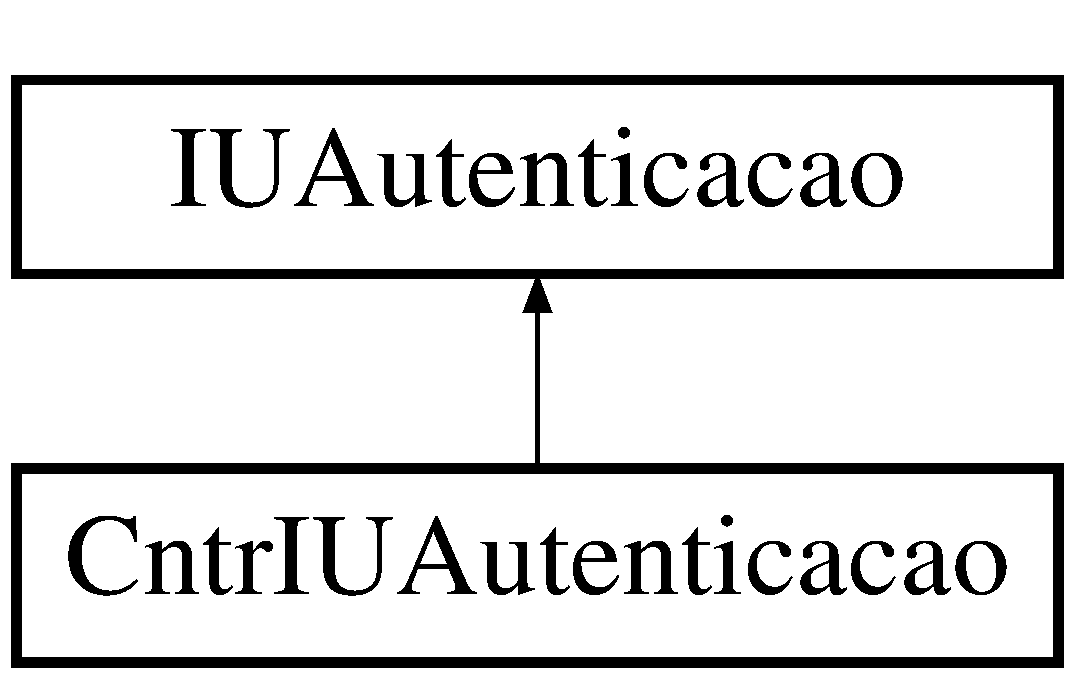
\includegraphics[height=2.000000cm]{class_cntr_i_u_autenticacao}
\end{center}
\end{figure}
\subsection*{Public Member Functions}
\begin{DoxyCompactItemize}
\item 
\hypertarget{class_cntr_i_u_autenticacao_a753ca57d7de28b1535696df732b6fba6}{}\label{class_cntr_i_u_autenticacao_a753ca57d7de28b1535696df732b6fba6} 
\hyperlink{class_resultado_autenticacao}{Resultado\+Autenticacao} {\bfseries autenticar} ()  throw (runtime\+\_\+error)
\item 
\hypertarget{class_cntr_i_u_autenticacao_a4fceb69522f4d8390b699d06742a6364}{}\label{class_cntr_i_u_autenticacao_a4fceb69522f4d8390b699d06742a6364} 
void {\bfseries set\+Cntr\+L\+N\+Autenticacao} (\hyperlink{class_i_l_n_autenticacao}{I\+L\+N\+Autenticacao} $\ast$cntr\+L\+N\+Autenticacao)
\end{DoxyCompactItemize}


\subsection{Detailed Description}
Classe respons�vel por autentica��o na interface. 

Cont�m os prot�tipos dos m�todos utilizados para autentica��o do usu�rio na interface. 

The documentation for this class was generated from the following file\+:\begin{DoxyCompactItemize}
\item 
\hyperlink{_controladoras_8h}{Controladoras.\+h}\end{DoxyCompactItemize}

\hypertarget{class_cntr_i_u_desenvolvedor}{}\section{Cntr\+I\+U\+Desenvolvedor Class Reference}
\label{class_cntr_i_u_desenvolvedor}\index{Cntr\+I\+U\+Desenvolvedor@{Cntr\+I\+U\+Desenvolvedor}}


Classe respons�vel pelo controle do desenvolvedor na interface.  




{\ttfamily \#include $<$Controladoras.\+h$>$}

Inheritance diagram for Cntr\+I\+U\+Desenvolvedor\+:\begin{figure}[H]
\begin{center}
\leavevmode
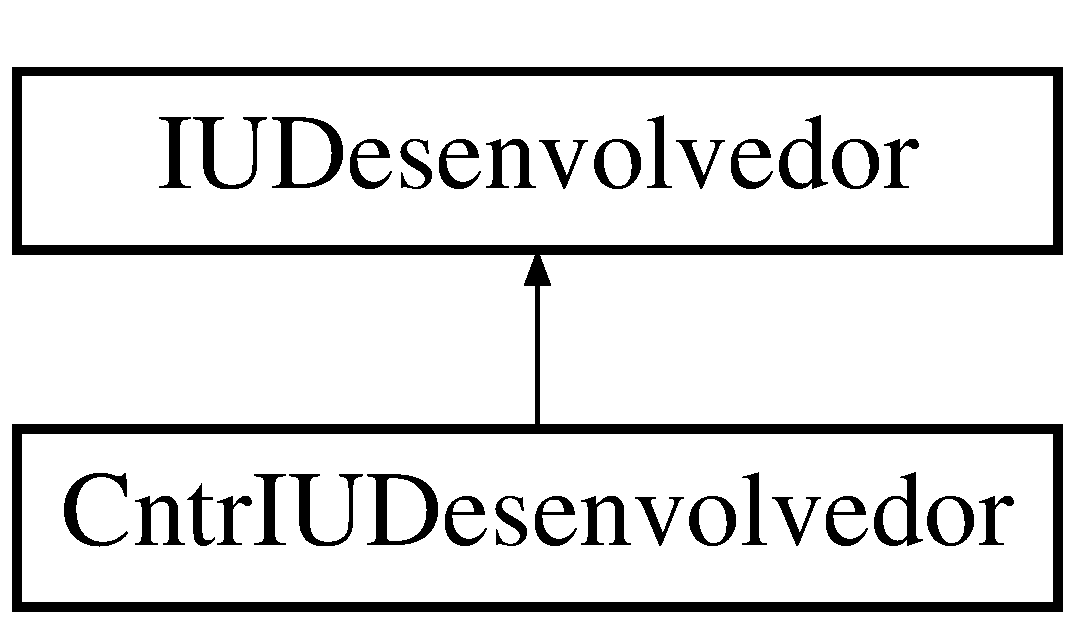
\includegraphics[height=2.000000cm]{class_cntr_i_u_desenvolvedor}
\end{center}
\end{figure}
\subsection*{Public Member Functions}
\begin{DoxyCompactItemize}
\item 
\hypertarget{class_cntr_i_u_desenvolvedor_afd1979803f4e52250c7e6ec14575ed76}{}\label{class_cntr_i_u_desenvolvedor_afd1979803f4e52250c7e6ec14575ed76} 
void {\bfseries executar} (const \hyperlink{class_matricula}{Matricula} \&)  throw (runtime\+\_\+error)
\item 
\hypertarget{class_cntr_i_u_desenvolvedor_a4c972d30297f322c332899385ddb1cc6}{}\label{class_cntr_i_u_desenvolvedor_a4c972d30297f322c332899385ddb1cc6} 
void {\bfseries set\+Cntr\+L\+N\+Desenvolvedor} (\hyperlink{class_i_l_n_desenvolvedor}{I\+L\+N\+Desenvolvedor} $\ast$)
\end{DoxyCompactItemize}
\subsection*{Static Public Member Functions}
\begin{DoxyCompactItemize}
\item 
\hypertarget{class_cntr_i_u_desenvolvedor_afae6ff36b3daecb4ace40755fc170e54}{}\label{class_cntr_i_u_desenvolvedor_afae6ff36b3daecb4ace40755fc170e54} 
static \hyperlink{class_cntr_i_u_desenvolvedor}{Cntr\+I\+U\+Desenvolvedor} $\ast$ {\bfseries instanciar} ()
\end{DoxyCompactItemize}


\subsection{Detailed Description}
Classe respons�vel pelo controle do desenvolvedor na interface. 

Cont�m os prot�tipos dos m�todos utilizados para controlar desenvolvedores na interface. 

The documentation for this class was generated from the following file\+:\begin{DoxyCompactItemize}
\item 
\hyperlink{_controladoras_8h}{Controladoras.\+h}\end{DoxyCompactItemize}

\hypertarget{class_cntr_i_u_gerente_projeto}{}\section{Cntr\+I\+U\+Gerente\+Projeto Class Reference}
\label{class_cntr_i_u_gerente_projeto}\index{Cntr\+I\+U\+Gerente\+Projeto@{Cntr\+I\+U\+Gerente\+Projeto}}


Classe respons�vel pelo controle do gerente de projeto na interface.  




{\ttfamily \#include $<$Controladoras.\+h$>$}

Inheritance diagram for Cntr\+I\+U\+Gerente\+Projeto\+:\begin{figure}[H]
\begin{center}
\leavevmode
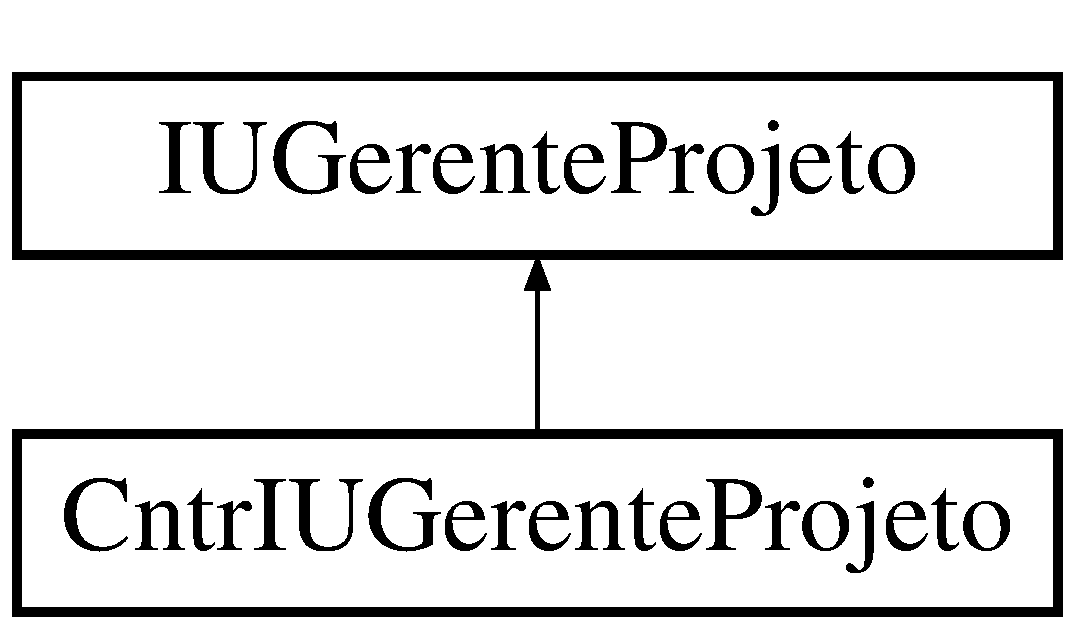
\includegraphics[height=2.000000cm]{class_cntr_i_u_gerente_projeto}
\end{center}
\end{figure}
\subsection*{Classes}
\begin{DoxyCompactItemize}
\item 
class \hyperlink{class_cntr_i_u_gerente_projeto_1_1_cntr_edicao}{Cntr\+Edicao}
\begin{DoxyCompactList}\small\item\em Classe interna respons�vel pela edi��o do gerente de projeto na interface l�gica de neg�cio. \end{DoxyCompactList}\item 
class \hyperlink{class_cntr_i_u_gerente_projeto_1_1_cntr_inclusao}{Cntr\+Inclusao}
\begin{DoxyCompactList}\small\item\em Classe interna respons�vel pela inclus�o do gerente de projeto na interface l�gica de neg�cio. \end{DoxyCompactList}\item 
class \hyperlink{class_cntr_i_u_gerente_projeto_1_1_cntr_pesquisa}{Cntr\+Pesquisa}
\begin{DoxyCompactList}\small\item\em Classe interna respons�vel pela pesquisa do gerente de projeto na interface l�gica de neg�cio. \end{DoxyCompactList}\item 
class \hyperlink{class_cntr_i_u_gerente_projeto_1_1_cntr_remocao}{Cntr\+Remocao}
\begin{DoxyCompactList}\small\item\em Classe interna respons�vel pela remo��o do gerente de projeto na interface l�gica de neg�cio. \end{DoxyCompactList}\end{DoxyCompactItemize}
\subsection*{Public Member Functions}
\begin{DoxyCompactItemize}
\item 
\hypertarget{class_cntr_i_u_gerente_projeto_aa97b82be7ce3993cffa6de609aed4880}{}\label{class_cntr_i_u_gerente_projeto_aa97b82be7ce3993cffa6de609aed4880} 
void {\bfseries executar} (const \hyperlink{class_matricula}{Matricula} \&)  throw (runtime\+\_\+error)
\item 
\hypertarget{class_cntr_i_u_gerente_projeto_a9a87e197155252ab52afea0bf034b164}{}\label{class_cntr_i_u_gerente_projeto_a9a87e197155252ab52afea0bf034b164} 
void {\bfseries set\+Cntr\+L\+N\+Gerente\+Projeto} (\hyperlink{class_i_l_n_gerente_projeto}{I\+L\+N\+Gerente\+Projeto} $\ast$cntr\+L\+N\+Gerente\+Projeto)
\end{DoxyCompactItemize}


\subsection{Detailed Description}
Classe respons�vel pelo controle do gerente de projeto na interface. 

Cont�m os prot�tipos dos m�todos utilizados para controlar gerentes de projetos na interface. 

The documentation for this class was generated from the following file\+:\begin{DoxyCompactItemize}
\item 
\hyperlink{_controladoras_8h}{Controladoras.\+h}\end{DoxyCompactItemize}

\hypertarget{class_cntr_i_u_gerente_sistema}{}\section{Cntr\+I\+U\+Gerente\+Sistema Class Reference}
\label{class_cntr_i_u_gerente_sistema}\index{Cntr\+I\+U\+Gerente\+Sistema@{Cntr\+I\+U\+Gerente\+Sistema}}


Classe respons�vel pelo controle do gerente de sistema na interface.  




{\ttfamily \#include $<$Controladoras.\+h$>$}

Inheritance diagram for Cntr\+I\+U\+Gerente\+Sistema\+:\begin{figure}[H]
\begin{center}
\leavevmode
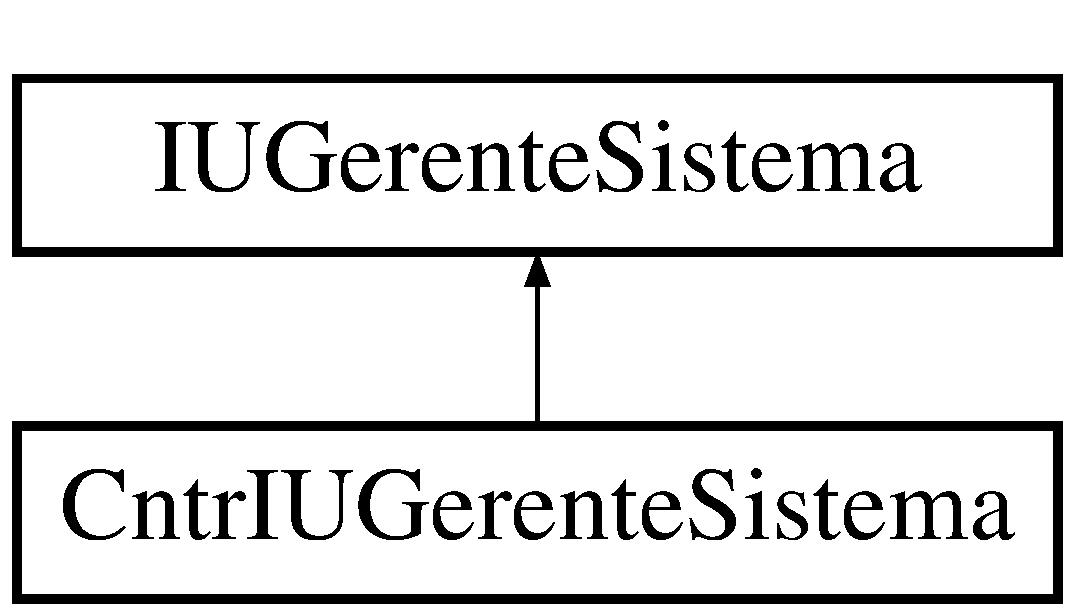
\includegraphics[height=2.000000cm]{class_cntr_i_u_gerente_sistema}
\end{center}
\end{figure}
\subsection*{Classes}
\begin{DoxyCompactItemize}
\item 
class \hyperlink{class_cntr_i_u_gerente_sistema_1_1_cntr_edicao}{Cntr\+Edicao}
\item 
class \hyperlink{class_cntr_i_u_gerente_sistema_1_1_cntr_inclusao}{Cntr\+Inclusao}
\begin{DoxyCompactList}\small\item\em Classe interna respons�vel pela inclus�o do gerente de sistema na interface l�gica de neg�cio. \end{DoxyCompactList}\item 
class \hyperlink{class_cntr_i_u_gerente_sistema_1_1_cntr_pesquisa}{Cntr\+Pesquisa}
\begin{DoxyCompactList}\small\item\em Classe interna respons�vel pela pesquisa do gerente de sistema na interface l�gica de neg�cio. \end{DoxyCompactList}\item 
class \hyperlink{class_cntr_i_u_gerente_sistema_1_1_cntr_remocao}{Cntr\+Remocao}
\begin{DoxyCompactList}\small\item\em Classe interna respons�vel pela remo�ao do gerente de sistema na interface l�gica de neg�cio. \end{DoxyCompactList}\end{DoxyCompactItemize}
\subsection*{Public Member Functions}
\begin{DoxyCompactItemize}
\item 
\hypertarget{class_cntr_i_u_gerente_sistema_a7c692bc34ab54d479d135c1e139d4f16}{}\label{class_cntr_i_u_gerente_sistema_a7c692bc34ab54d479d135c1e139d4f16} 
void {\bfseries executar} (const \hyperlink{class_matricula}{Matricula} \&)  throw (runtime\+\_\+error)
\item 
\hypertarget{class_cntr_i_u_gerente_sistema_a1bfdec59d518a4a5b3d04bda1241c9f9}{}\label{class_cntr_i_u_gerente_sistema_a1bfdec59d518a4a5b3d04bda1241c9f9} 
void {\bfseries set\+Cntr\+L\+N\+Gerente\+Sistema} (\hyperlink{class_i_l_n_gerente_sistema}{I\+L\+N\+Gerente\+Sistema} $\ast$cntr\+L\+N\+Gerente\+Sistema)
\end{DoxyCompactItemize}


\subsection{Detailed Description}
Classe respons�vel pelo controle do gerente de sistema na interface. 

Cont�m os prot�tipos dos m�todos utilizados para controlar gerentes de sistema na interface. 

The documentation for this class was generated from the following file\+:\begin{DoxyCompactItemize}
\item 
\hyperlink{_controladoras_8h}{Controladoras.\+h}\end{DoxyCompactItemize}

\hypertarget{class_cntr_i_u_projeto}{}\section{Cntr\+I\+U\+Projeto Class Reference}
\label{class_cntr_i_u_projeto}\index{Cntr\+I\+U\+Projeto@{Cntr\+I\+U\+Projeto}}


Classe respons�vel pelo controle do projeto na interface.  




{\ttfamily \#include $<$Controladoras.\+h$>$}

Inheritance diagram for Cntr\+I\+U\+Projeto\+:\begin{figure}[H]
\begin{center}
\leavevmode
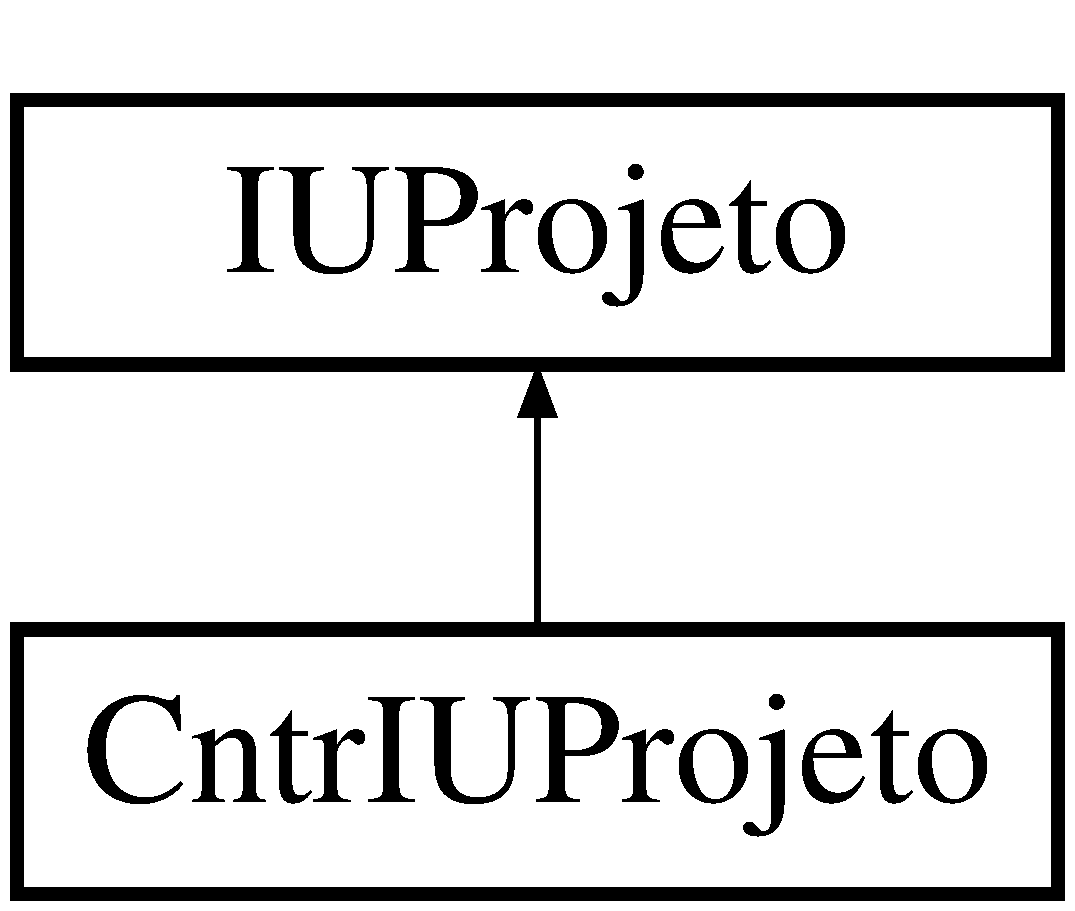
\includegraphics[height=2.000000cm]{class_cntr_i_u_projeto}
\end{center}
\end{figure}
\subsection*{Public Member Functions}
\begin{DoxyCompactItemize}
\item 
\hypertarget{class_cntr_i_u_projeto_af27417689ab83098d43b3fddb1ebf2aa}{}\label{class_cntr_i_u_projeto_af27417689ab83098d43b3fddb1ebf2aa} 
void {\bfseries executar} (const \hyperlink{class_matricula}{Matricula} \&)  throw (runtime\+\_\+error)
\item 
\hypertarget{class_cntr_i_u_projeto_afc6d5bbfc42995d6707aca63c292c6a7}{}\label{class_cntr_i_u_projeto_afc6d5bbfc42995d6707aca63c292c6a7} 
void {\bfseries set\+Cntr\+L\+N\+Projeto} (\hyperlink{class_i_l_n_projeto}{I\+L\+N\+Projeto} $\ast$cntr\+L\+N\+Projeto)
\end{DoxyCompactItemize}


\subsection{Detailed Description}
Classe respons�vel pelo controle do projeto na interface. 

Cont�m os prot�tipos dos m�todos utilizados para controlar projetos na interface. 

The documentation for this class was generated from the following file\+:\begin{DoxyCompactItemize}
\item 
\hyperlink{_controladoras_8h}{Controladoras.\+h}\end{DoxyCompactItemize}

\hypertarget{class_cntr_i_u_gerente_sistema_1_1_cntr_pesquisa}{}\section{Cntr\+I\+U\+Gerente\+Sistema\+:\+:Cntr\+Pesquisa Class Reference}
\label{class_cntr_i_u_gerente_sistema_1_1_cntr_pesquisa}\index{Cntr\+I\+U\+Gerente\+Sistema\+::\+Cntr\+Pesquisa@{Cntr\+I\+U\+Gerente\+Sistema\+::\+Cntr\+Pesquisa}}


Classe interna respons�vel pela pesquisa do gerente de sistema na interface l�gica de neg�cio.  




{\ttfamily \#include $<$Controladoras.\+h$>$}

\subsection*{Public Member Functions}
\begin{DoxyCompactItemize}
\item 
\hypertarget{class_cntr_i_u_gerente_sistema_1_1_cntr_pesquisa_a6f93a1ed50c51048c916d35c905e1cd9}{}\label{class_cntr_i_u_gerente_sistema_1_1_cntr_pesquisa_a6f93a1ed50c51048c916d35c905e1cd9} 
void {\bfseries executar} (\hyperlink{class_i_l_n_gerente_sistema}{I\+L\+N\+Gerente\+Sistema} $\ast$)  throw (runtime\+\_\+error)
\end{DoxyCompactItemize}


\subsection{Detailed Description}
Classe interna respons�vel pela pesquisa do gerente de sistema na interface l�gica de neg�cio. 

Cont�m os prot�tipos dos m�todos utilizados para controlar a pesquisa de gerentes de sistema na interface l�gica de neg�cio. 

The documentation for this class was generated from the following file\+:\begin{DoxyCompactItemize}
\item 
\hyperlink{_controladoras_8h}{Controladoras.\+h}\end{DoxyCompactItemize}

\hypertarget{class_cntr_i_u_gerente_projeto_1_1_cntr_pesquisa}{}\section{Cntr\+I\+U\+Gerente\+Projeto\+:\+:Cntr\+Pesquisa Class Reference}
\label{class_cntr_i_u_gerente_projeto_1_1_cntr_pesquisa}\index{Cntr\+I\+U\+Gerente\+Projeto\+::\+Cntr\+Pesquisa@{Cntr\+I\+U\+Gerente\+Projeto\+::\+Cntr\+Pesquisa}}


Classe interna respons�vel pela pesquisa do gerente de projeto na interface l�gica de neg�cio.  




{\ttfamily \#include $<$Controladoras.\+h$>$}

\subsection*{Public Member Functions}
\begin{DoxyCompactItemize}
\item 
\hypertarget{class_cntr_i_u_gerente_projeto_1_1_cntr_pesquisa_a5ad097608c309a7b2f22c80cd12ea42a}{}\label{class_cntr_i_u_gerente_projeto_1_1_cntr_pesquisa_a5ad097608c309a7b2f22c80cd12ea42a} 
void {\bfseries executar} (\hyperlink{class_i_l_n_gerente_projeto}{I\+L\+N\+Gerente\+Projeto} $\ast$)  throw (runtime\+\_\+error)
\end{DoxyCompactItemize}


\subsection{Detailed Description}
Classe interna respons�vel pela pesquisa do gerente de projeto na interface l�gica de neg�cio. 

Cont�m os prot�tipos dos m�todos utilizados para controlar a pesquisa de gerentes de projetos na interface l�gica de neg�cio. 

The documentation for this class was generated from the following file\+:\begin{DoxyCompactItemize}
\item 
\hyperlink{_controladoras_8h}{Controladoras.\+h}\end{DoxyCompactItemize}

\hypertarget{class_cntr_i_u_gerente_projeto_1_1_cntr_remocao}{}\section{Cntr\+I\+U\+Gerente\+Projeto\+:\+:Cntr\+Remocao Class Reference}
\label{class_cntr_i_u_gerente_projeto_1_1_cntr_remocao}\index{Cntr\+I\+U\+Gerente\+Projeto\+::\+Cntr\+Remocao@{Cntr\+I\+U\+Gerente\+Projeto\+::\+Cntr\+Remocao}}


Classe interna respons�vel pela remo��o do gerente de projeto na interface l�gica de neg�cio.  




{\ttfamily \#include $<$Controladoras.\+h$>$}

\subsection*{Public Member Functions}
\begin{DoxyCompactItemize}
\item 
\hypertarget{class_cntr_i_u_gerente_projeto_1_1_cntr_remocao_a81af63249643b6e643bcf921d46f00dd}{}\label{class_cntr_i_u_gerente_projeto_1_1_cntr_remocao_a81af63249643b6e643bcf921d46f00dd} 
void {\bfseries executar} (\hyperlink{class_i_l_n_gerente_projeto}{I\+L\+N\+Gerente\+Projeto} $\ast$)  throw (runtime\+\_\+error)
\end{DoxyCompactItemize}


\subsection{Detailed Description}
Classe interna respons�vel pela remo��o do gerente de projeto na interface l�gica de neg�cio. 

Cont�m os prot�tipos dos m�todos utilizados para controlar a remo��o de gerentes de projetos na interface l�gica de neg�cio. 

The documentation for this class was generated from the following file\+:\begin{DoxyCompactItemize}
\item 
\hyperlink{_controladoras_8h}{Controladoras.\+h}\end{DoxyCompactItemize}

\hypertarget{class_cntr_i_u_gerente_sistema_1_1_cntr_remocao}{}\section{Cntr\+I\+U\+Gerente\+Sistema\+:\+:Cntr\+Remocao Class Reference}
\label{class_cntr_i_u_gerente_sistema_1_1_cntr_remocao}\index{Cntr\+I\+U\+Gerente\+Sistema\+::\+Cntr\+Remocao@{Cntr\+I\+U\+Gerente\+Sistema\+::\+Cntr\+Remocao}}


Classe interna respons�vel pela remo�ao do gerente de sistema na interface l�gica de neg�cio.  




{\ttfamily \#include $<$Controladoras.\+h$>$}

\subsection*{Public Member Functions}
\begin{DoxyCompactItemize}
\item 
\hypertarget{class_cntr_i_u_gerente_sistema_1_1_cntr_remocao_a3a7546ce42810306e29721675658e462}{}\label{class_cntr_i_u_gerente_sistema_1_1_cntr_remocao_a3a7546ce42810306e29721675658e462} 
void {\bfseries executar} (\hyperlink{class_i_l_n_gerente_sistema}{I\+L\+N\+Gerente\+Sistema} $\ast$)  throw (runtime\+\_\+error)
\end{DoxyCompactItemize}


\subsection{Detailed Description}
Classe interna respons�vel pela remo�ao do gerente de sistema na interface l�gica de neg�cio. 

Cont�m os prot�tipos dos m�todos utilizados para controlar a remo��o de gerentes de sistema na interface l�gica de neg�cio. 

The documentation for this class was generated from the following file\+:\begin{DoxyCompactItemize}
\item 
\hyperlink{_controladoras_8h}{Controladoras.\+h}\end{DoxyCompactItemize}

\hypertarget{class_codigo_projeto}{}\section{Codigo\+Projeto Class Reference}
\label{class_codigo_projeto}\index{Codigo\+Projeto@{Codigo\+Projeto}}


Classe que cont�m os principais m�todos do codigo do projeto do dominio.  




{\ttfamily \#include $<$Dominio.\+h$>$}

\subsection*{Public Member Functions}
\begin{DoxyCompactItemize}
\item 
\hypertarget{class_codigo_projeto_a24f268611c9fac90b9919b9ee29ed49a}{}\label{class_codigo_projeto_a24f268611c9fac90b9919b9ee29ed49a} 
{\bfseries Codigo\+Projeto} (string)
\item 
\hypertarget{class_codigo_projeto_a1daac1eeea7a69cda7751f418066c610}{}\label{class_codigo_projeto_a1daac1eeea7a69cda7751f418066c610} 
void {\bfseries set\+Codigo\+Projeto} (string)  throw (invalid\+\_\+argument)
\item 
\hypertarget{class_codigo_projeto_abfa8975350986401b874f5991d773ff2}{}\label{class_codigo_projeto_abfa8975350986401b874f5991d773ff2} 
string {\bfseries get\+Codigo\+Projeto} () const
\item 
\hypertarget{class_codigo_projeto_a6b5502fbb2f124b13b54fbf8ab7f79e7}{}\label{class_codigo_projeto_a6b5502fbb2f124b13b54fbf8ab7f79e7} 
void {\bfseries is\+Codigo\+Projeto\+Valid} (string)  throw (invalid\+\_\+argument)
\end{DoxyCompactItemize}


\subsection{Detailed Description}
Classe que cont�m os principais m�todos do codigo do projeto do dominio. 

Cont�m os prot�tipos dos m�todos do nome referente ao dom�nio do sistema. 

The documentation for this class was generated from the following file\+:\begin{DoxyCompactItemize}
\item 
\hyperlink{_dominio_8h}{Dominio.\+h}\end{DoxyCompactItemize}

\hypertarget{class_comando_banco_dados}{}\section{Comando\+Banco\+Dados Class Reference}
\label{class_comando_banco_dados}\index{Comando\+Banco\+Dados@{Comando\+Banco\+Dados}}


Classe que contém os principais métodos dos comandos do banco de dados.  




{\ttfamily \#include $<$Comandos.\+h$>$}

Inheritance diagram for Comando\+Banco\+Dados\+:\begin{figure}[H]
\begin{center}
\leavevmode
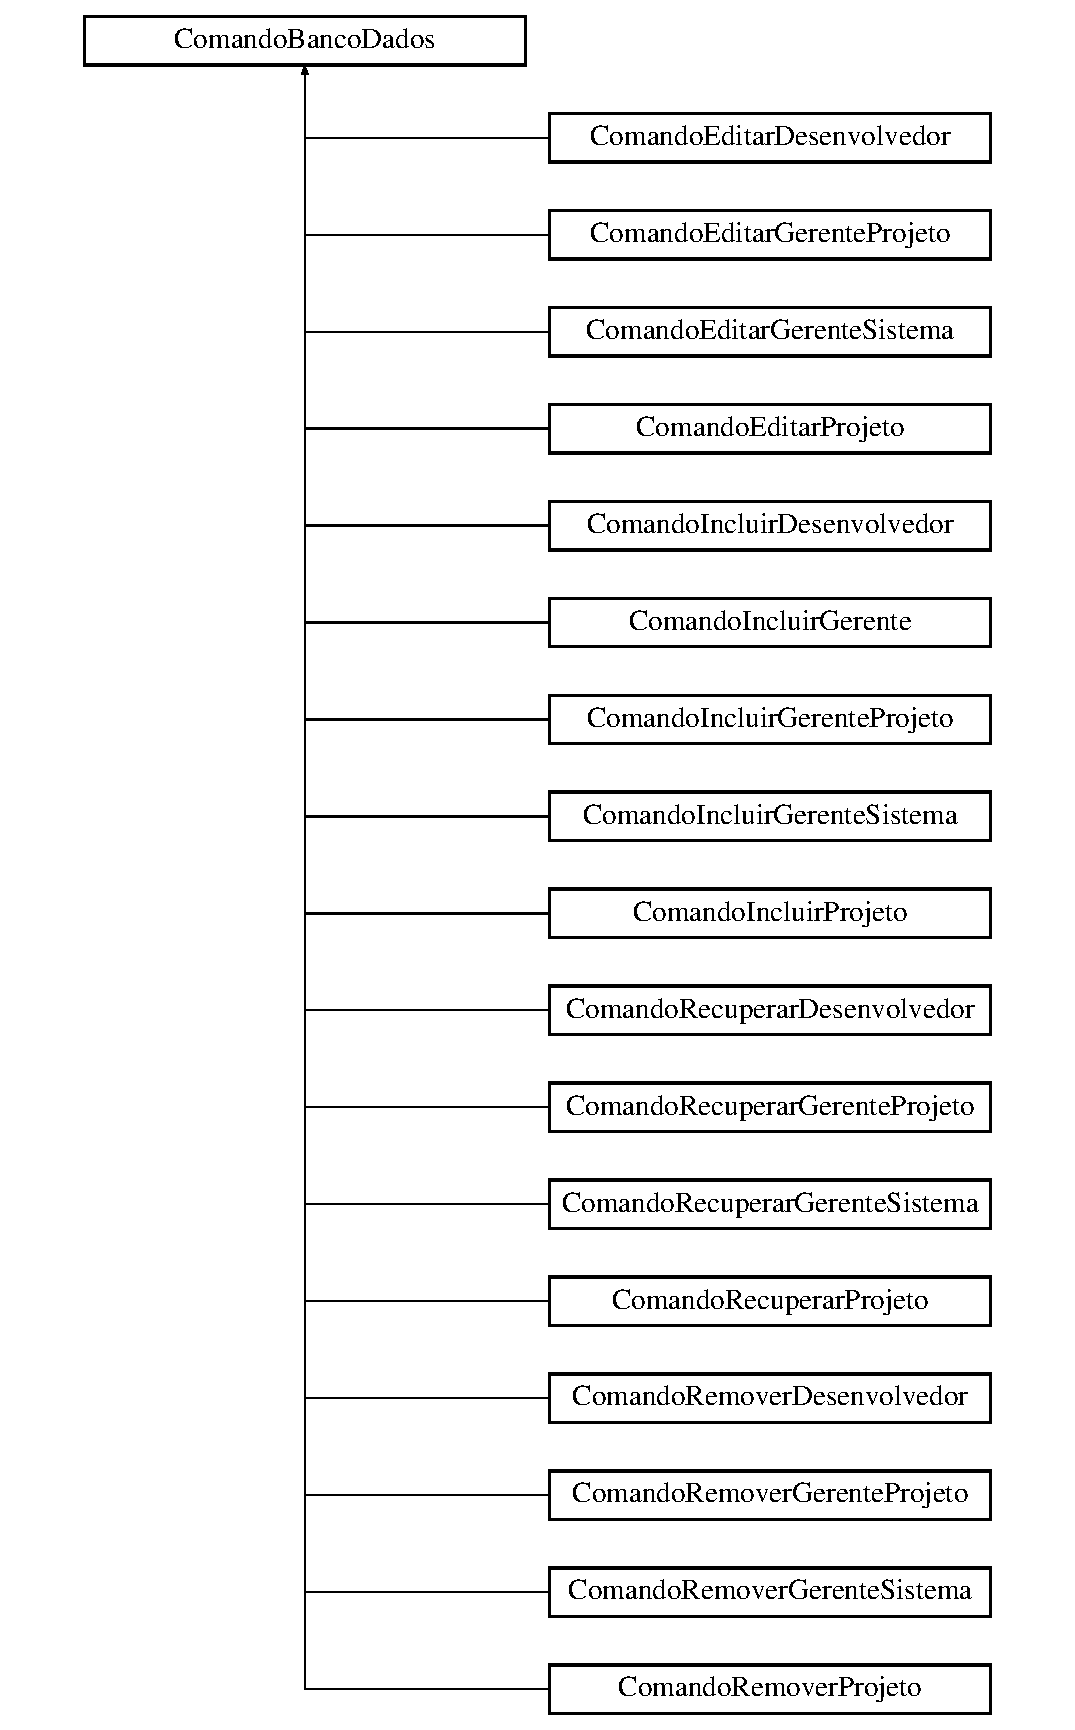
\includegraphics[height=12.000000cm]{class_comando_banco_dados}
\end{center}
\end{figure}
\subsection*{Public Member Functions}
\begin{DoxyCompactItemize}
\item 
\hypertarget{class_comando_banco_dados_a4f71e8d9f2b3e997645bc356a5473433}{}\label{class_comando_banco_dados_a4f71e8d9f2b3e997645bc356a5473433} 
virtual void {\bfseries executar} ()=0  throw (runtime\+\_\+error)
\item 
\hypertarget{class_comando_banco_dados_a4f71e8d9f2b3e997645bc356a5473433}{}\label{class_comando_banco_dados_a4f71e8d9f2b3e997645bc356a5473433} 
virtual void {\bfseries executar} ()=0  throw (runtime\+\_\+error)
\end{DoxyCompactItemize}


\subsection{Detailed Description}
Classe que contém os principais métodos dos comandos do banco de dados. 

Contém os protótipos dos métodos utilizados nas outras classes que se comunicam com o banco de dados. 

The documentation for this class was generated from the following files\+:\begin{DoxyCompactItemize}
\item 
\hyperlink{_comandos_8h}{Comandos.\+h}\item 
\hyperlink{_lnegocio_8h}{Lnegocio.\+h}\end{DoxyCompactItemize}

\hypertarget{class_comando_editar_desenvolvedor}{}\section{Comando\+Editar\+Desenvolvedor Class Reference}
\label{class_comando_editar_desenvolvedor}\index{Comando\+Editar\+Desenvolvedor@{Comando\+Editar\+Desenvolvedor}}


Classe responsável por\+: Editar desenvolvedor.  




{\ttfamily \#include $<$Comandos.\+h$>$}

Inheritance diagram for Comando\+Editar\+Desenvolvedor\+:\begin{figure}[H]
\begin{center}
\leavevmode
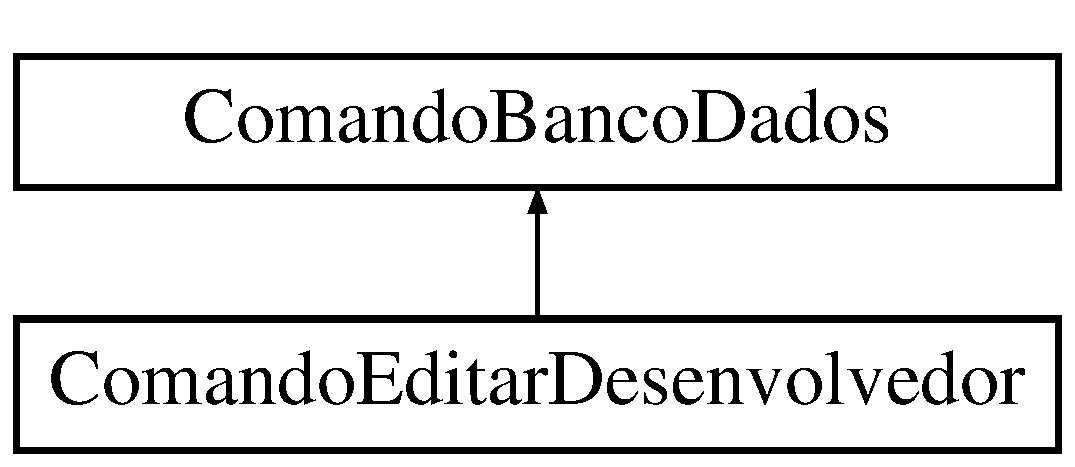
\includegraphics[height=2.000000cm]{class_comando_editar_desenvolvedor}
\end{center}
\end{figure}
\subsection*{Public Member Functions}
\begin{DoxyCompactItemize}
\item 
\hypertarget{class_comando_editar_desenvolvedor_ae4949af13a1df3694b1a4fea59064326}{}\label{class_comando_editar_desenvolvedor_ae4949af13a1df3694b1a4fea59064326} 
void {\bfseries executar} ()  throw (runtime\+\_\+error)
\end{DoxyCompactItemize}


\subsection{Detailed Description}
Classe responsável por\+: Editar desenvolvedor. 

Contém o protótipo do método responsável pelo comando do banco de dados, exclusivo do Gerente de \hyperlink{class_projeto}{Projeto}, de Editar um desenvolvedor. 

The documentation for this class was generated from the following file\+:\begin{DoxyCompactItemize}
\item 
\hyperlink{_comandos_8h}{Comandos.\+h}\end{DoxyCompactItemize}

\hypertarget{class_comando_editar_gerente}{}\section{Comando\+Editar\+Gerente Class Reference}
\label{class_comando_editar_gerente}\index{Comando\+Editar\+Gerente@{Comando\+Editar\+Gerente}}


The documentation for this class was generated from the following file\+:\begin{DoxyCompactItemize}
\item 
\hyperlink{_lnegocio_8h}{Lnegocio.\+h}\end{DoxyCompactItemize}

\hypertarget{class_comando_editar_gerente_projeto}{}\section{Comando\+Editar\+Gerente\+Projeto Class Reference}
\label{class_comando_editar_gerente_projeto}\index{Comando\+Editar\+Gerente\+Projeto@{Comando\+Editar\+Gerente\+Projeto}}


Classe responsável por\+: Editar Gerente de projeto.  




{\ttfamily \#include $<$Comandos.\+h$>$}

Inheritance diagram for Comando\+Editar\+Gerente\+Projeto\+:\begin{figure}[H]
\begin{center}
\leavevmode
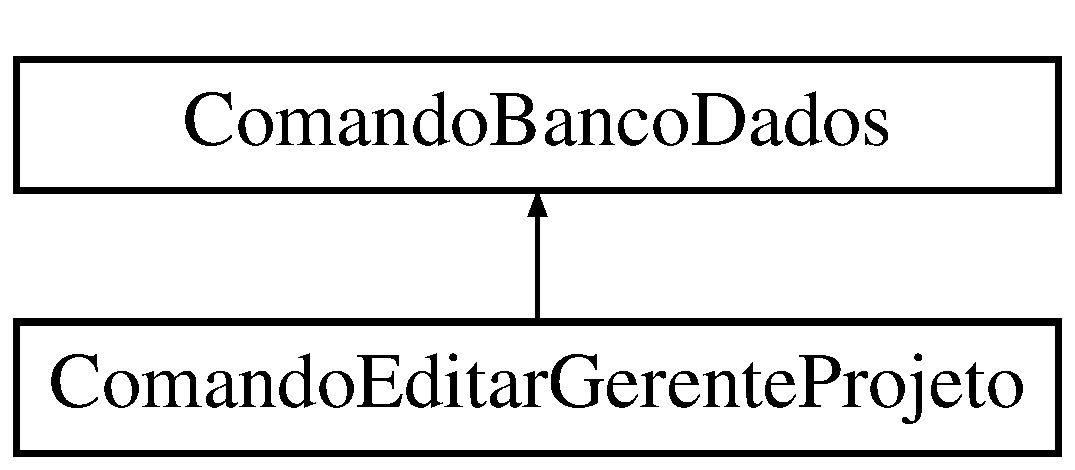
\includegraphics[height=2.000000cm]{class_comando_editar_gerente_projeto}
\end{center}
\end{figure}
\subsection*{Public Member Functions}
\begin{DoxyCompactItemize}
\item 
\hypertarget{class_comando_editar_gerente_projeto_ad3aa8ca7e9bf932742f415e79f324c40}{}\label{class_comando_editar_gerente_projeto_ad3aa8ca7e9bf932742f415e79f324c40} 
void {\bfseries executar} ()  throw (runtime\+\_\+error)
\end{DoxyCompactItemize}


\subsection{Detailed Description}
Classe responsável por\+: Editar Gerente de projeto. 

Contém o protótipo do método responsável pelo comando do banco de dados de editar um gerente de projeto. 

The documentation for this class was generated from the following file\+:\begin{DoxyCompactItemize}
\item 
\hyperlink{_comandos_8h}{Comandos.\+h}\end{DoxyCompactItemize}

\hypertarget{class_comando_editar_gerente_sistema}{}\section{Comando\+Editar\+Gerente\+Sistema Class Reference}
\label{class_comando_editar_gerente_sistema}\index{Comando\+Editar\+Gerente\+Sistema@{Comando\+Editar\+Gerente\+Sistema}}


Classe responsável por\+: Editar Gerente de sistema.  




{\ttfamily \#include $<$Comandos.\+h$>$}

Inheritance diagram for Comando\+Editar\+Gerente\+Sistema\+:\begin{figure}[H]
\begin{center}
\leavevmode
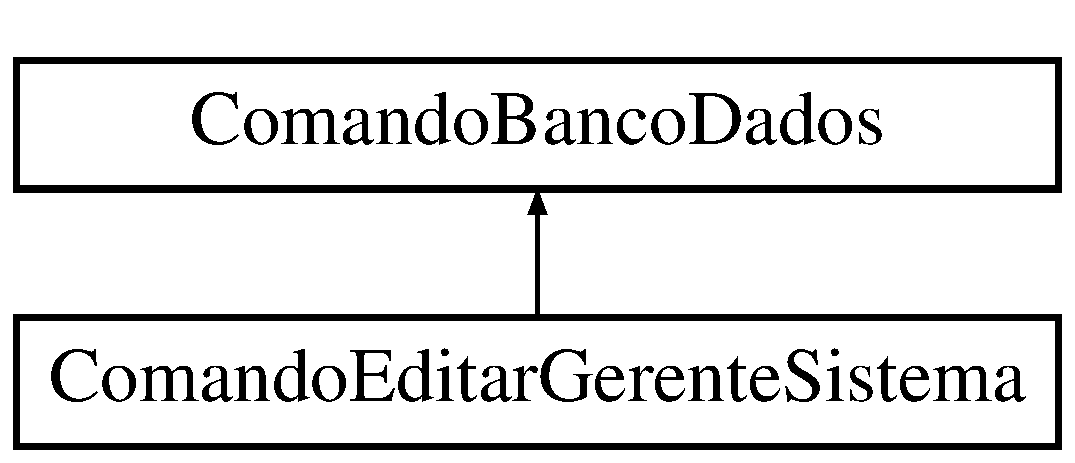
\includegraphics[height=2.000000cm]{class_comando_editar_gerente_sistema}
\end{center}
\end{figure}
\subsection*{Public Member Functions}
\begin{DoxyCompactItemize}
\item 
\hypertarget{class_comando_editar_gerente_sistema_ac84b2f4aed833ba46b19bcc230f03b3f}{}\label{class_comando_editar_gerente_sistema_ac84b2f4aed833ba46b19bcc230f03b3f} 
void {\bfseries executar} ()  throw (runtime\+\_\+error)
\end{DoxyCompactItemize}


\subsection{Detailed Description}
Classe responsável por\+: Editar Gerente de sistema. 

Contém o protótipo do método responsável pelo comando do banco de dados de editar um gerente de sistema. 

The documentation for this class was generated from the following file\+:\begin{DoxyCompactItemize}
\item 
\hyperlink{_comandos_8h}{Comandos.\+h}\end{DoxyCompactItemize}

\hypertarget{class_comando_editar_projeto}{}\section{Comando\+Editar\+Projeto Class Reference}
\label{class_comando_editar_projeto}\index{Comando\+Editar\+Projeto@{Comando\+Editar\+Projeto}}


Classe responsável por\+: Editar projeto.  




{\ttfamily \#include $<$Comandos.\+h$>$}

Inheritance diagram for Comando\+Editar\+Projeto\+:\begin{figure}[H]
\begin{center}
\leavevmode
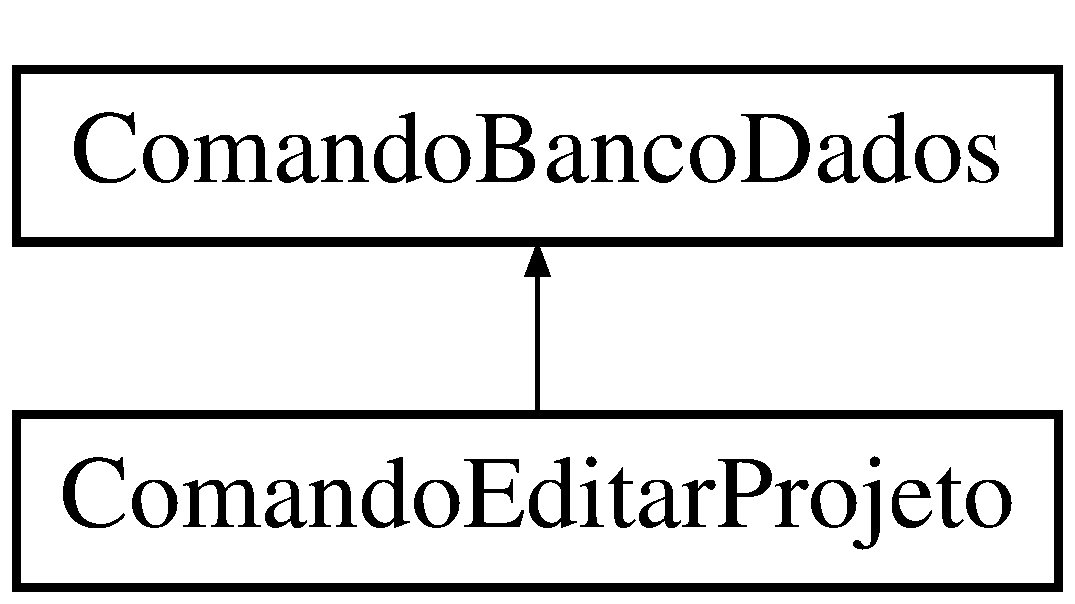
\includegraphics[height=2.000000cm]{class_comando_editar_projeto}
\end{center}
\end{figure}
\subsection*{Public Member Functions}
\begin{DoxyCompactItemize}
\item 
\hypertarget{class_comando_editar_projeto_a8ce95f26c60777abd0cad6426c913f6b}{}\label{class_comando_editar_projeto_a8ce95f26c60777abd0cad6426c913f6b} 
void {\bfseries executar} ()  throw (runtime\+\_\+error)
\end{DoxyCompactItemize}


\subsection{Detailed Description}
Classe responsável por\+: Editar projeto. 

Contém o protótipo do método responsável pelo comando do banco de dados, exclusivo do Gerente de \hyperlink{class_projeto}{Projeto}, de editar um projeto. 

The documentation for this class was generated from the following file\+:\begin{DoxyCompactItemize}
\item 
\hyperlink{_comandos_8h}{Comandos.\+h}\end{DoxyCompactItemize}

\hypertarget{class_comando_incluir_desenvolvedor}{}\section{Comando\+Incluir\+Desenvolvedor Class Reference}
\label{class_comando_incluir_desenvolvedor}\index{Comando\+Incluir\+Desenvolvedor@{Comando\+Incluir\+Desenvolvedor}}


Classe responsável por\+: Incluir desenvolvedor.  




{\ttfamily \#include $<$Comandos.\+h$>$}

Inheritance diagram for Comando\+Incluir\+Desenvolvedor\+:\begin{figure}[H]
\begin{center}
\leavevmode
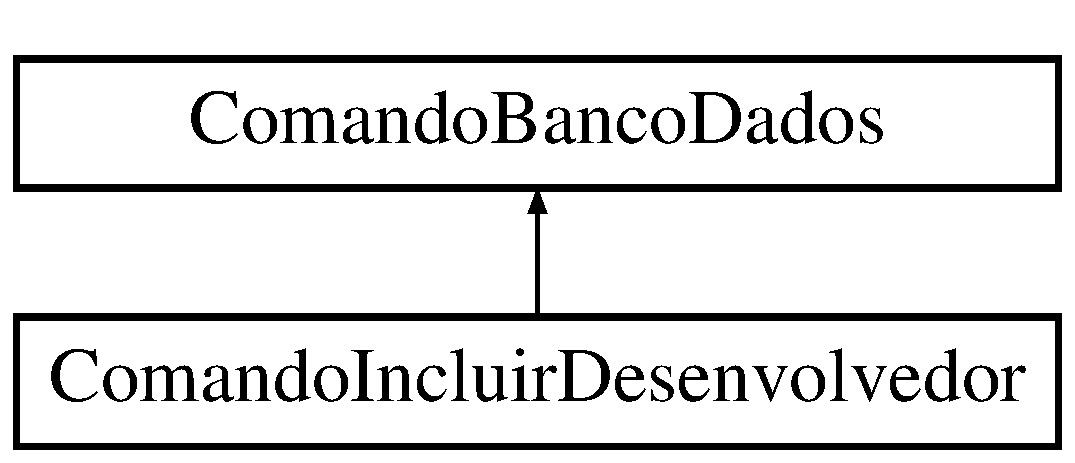
\includegraphics[height=2.000000cm]{class_comando_incluir_desenvolvedor}
\end{center}
\end{figure}
\subsection*{Public Member Functions}
\begin{DoxyCompactItemize}
\item 
\hypertarget{class_comando_incluir_desenvolvedor_a03138e5bdb37d0fd6da8bc25e002cbe7}{}\label{class_comando_incluir_desenvolvedor_a03138e5bdb37d0fd6da8bc25e002cbe7} 
void {\bfseries executar} ()  throw (runtime\+\_\+error)
\end{DoxyCompactItemize}


\subsection{Detailed Description}
Classe responsável por\+: Incluir desenvolvedor. 

Contém o protótipo do método responsável pelo comando do banco de dados, exclusivo do Gerente de \hyperlink{class_projeto}{Projeto}, de incluir um desenvolvedor. 

The documentation for this class was generated from the following file\+:\begin{DoxyCompactItemize}
\item 
\hyperlink{_comandos_8h}{Comandos.\+h}\end{DoxyCompactItemize}

\hypertarget{class_comando_incluir_gerente}{}\section{Comando\+Incluir\+Gerente Class Reference}
\label{class_comando_incluir_gerente}\index{Comando\+Incluir\+Gerente@{Comando\+Incluir\+Gerente}}


Classe responsável por\+: Incluir Gerente de projeto.  




{\ttfamily \#include $<$Lnegocio.\+h$>$}

Inheritance diagram for Comando\+Incluir\+Gerente\+:\begin{figure}[H]
\begin{center}
\leavevmode
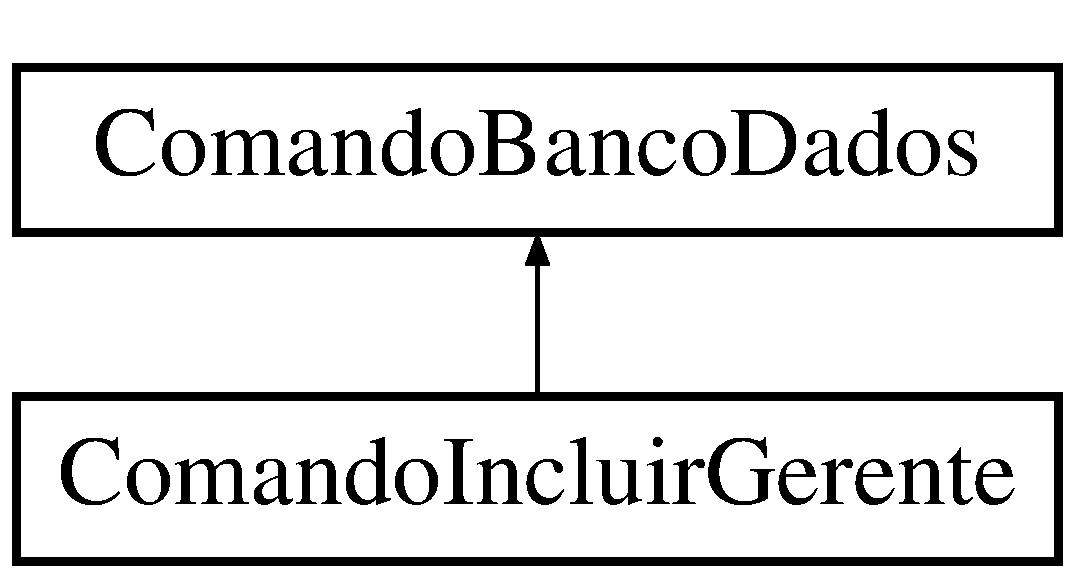
\includegraphics[height=2.000000cm]{class_comando_incluir_gerente}
\end{center}
\end{figure}
\subsection*{Public Member Functions}
\begin{DoxyCompactItemize}
\item 
\hypertarget{class_comando_incluir_gerente_a5f879ccd2330c3f6ef9b9af0dee2b54e}{}\label{class_comando_incluir_gerente_a5f879ccd2330c3f6ef9b9af0dee2b54e} 
void {\bfseries executar} ()  throw (runtime\+\_\+error)
\end{DoxyCompactItemize}


\subsection{Detailed Description}
Classe responsável por\+: Incluir Gerente de projeto. 

Contém o protótipo do método responsável pelo comando do banco de dados de incluir novo gerente de projeto. 

The documentation for this class was generated from the following file\+:\begin{DoxyCompactItemize}
\item 
\hyperlink{_lnegocio_8h}{Lnegocio.\+h}\end{DoxyCompactItemize}

\hypertarget{class_comando_incluir_gerente_projeto}{}\section{Comando\+Incluir\+Gerente\+Projeto Class Reference}
\label{class_comando_incluir_gerente_projeto}\index{Comando\+Incluir\+Gerente\+Projeto@{Comando\+Incluir\+Gerente\+Projeto}}


Classe responsável por\+: Incluir Gerente de projeto.  




{\ttfamily \#include $<$Comandos.\+h$>$}

Inheritance diagram for Comando\+Incluir\+Gerente\+Projeto\+:\begin{figure}[H]
\begin{center}
\leavevmode
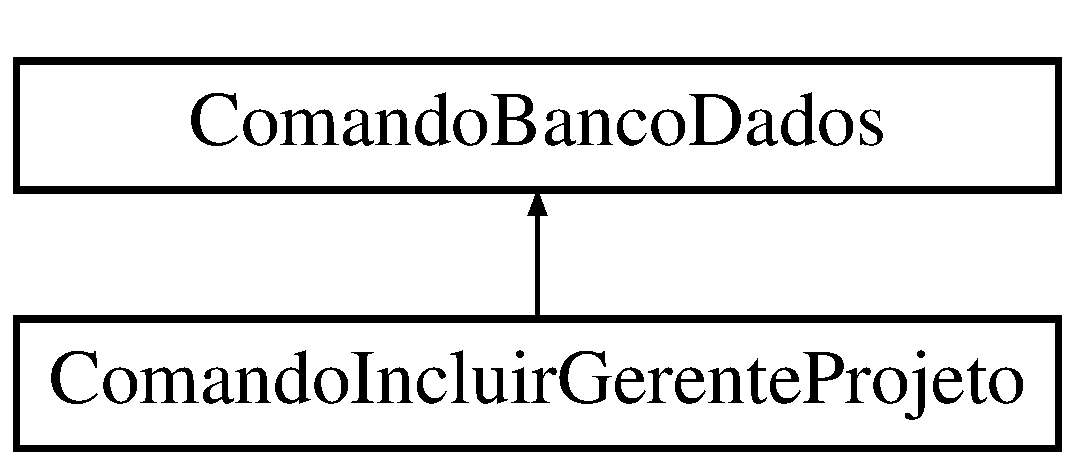
\includegraphics[height=2.000000cm]{class_comando_incluir_gerente_projeto}
\end{center}
\end{figure}
\subsection*{Public Member Functions}
\begin{DoxyCompactItemize}
\item 
\hypertarget{class_comando_incluir_gerente_projeto_aa2335f5e8292f9d9a0aa0344cecb72d9}{}\label{class_comando_incluir_gerente_projeto_aa2335f5e8292f9d9a0aa0344cecb72d9} 
void {\bfseries executar} ()  throw (runtime\+\_\+error)
\end{DoxyCompactItemize}


\subsection{Detailed Description}
Classe responsável por\+: Incluir Gerente de projeto. 

Contém o protótipo do método responsável pelo comando do banco de dados de incluir um gerente de projeto. 

The documentation for this class was generated from the following file\+:\begin{DoxyCompactItemize}
\item 
\hyperlink{_comandos_8h}{Comandos.\+h}\end{DoxyCompactItemize}

\hypertarget{class_comando_incluir_gerente_sistema}{}\section{Comando\+Incluir\+Gerente\+Sistema Class Reference}
\label{class_comando_incluir_gerente_sistema}\index{Comando\+Incluir\+Gerente\+Sistema@{Comando\+Incluir\+Gerente\+Sistema}}


Classe responsável por\+: Incluir Gerente de sistema.  




{\ttfamily \#include $<$Comandos.\+h$>$}

Inheritance diagram for Comando\+Incluir\+Gerente\+Sistema\+:\begin{figure}[H]
\begin{center}
\leavevmode
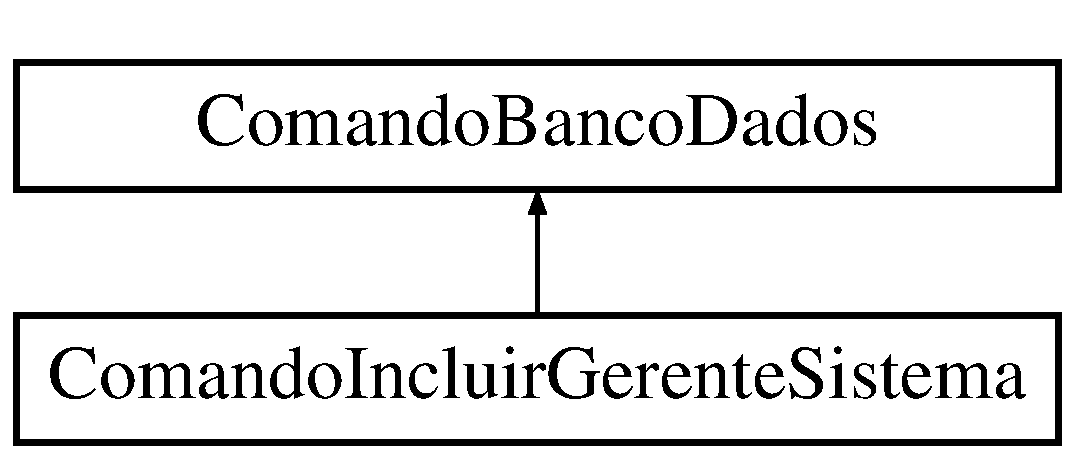
\includegraphics[height=2.000000cm]{class_comando_incluir_gerente_sistema}
\end{center}
\end{figure}
\subsection*{Public Member Functions}
\begin{DoxyCompactItemize}
\item 
\hypertarget{class_comando_incluir_gerente_sistema_a700ab7da317009ed1de092fb35fd38fd}{}\label{class_comando_incluir_gerente_sistema_a700ab7da317009ed1de092fb35fd38fd} 
void {\bfseries executar} ()  throw (runtime\+\_\+error)
\end{DoxyCompactItemize}


\subsection{Detailed Description}
Classe responsável por\+: Incluir Gerente de sistema. 

Contém o protótipo do método responsável pelo comando do banco de dados de incluir um gerente de sistema. 

The documentation for this class was generated from the following file\+:\begin{DoxyCompactItemize}
\item 
\hyperlink{_comandos_8h}{Comandos.\+h}\end{DoxyCompactItemize}

\hypertarget{class_comando_incluir_projeto}{}\section{Comando\+Incluir\+Projeto Class Reference}
\label{class_comando_incluir_projeto}\index{Comando\+Incluir\+Projeto@{Comando\+Incluir\+Projeto}}


Classe responsável por\+: Incluir projeto.  




{\ttfamily \#include $<$Comandos.\+h$>$}

Inheritance diagram for Comando\+Incluir\+Projeto\+:\begin{figure}[H]
\begin{center}
\leavevmode
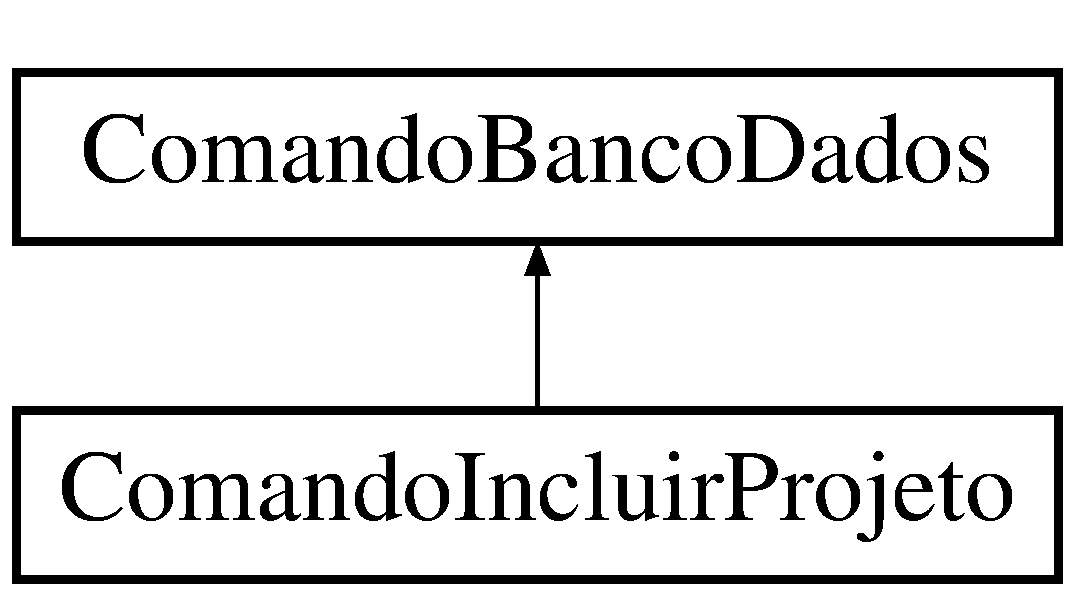
\includegraphics[height=2.000000cm]{class_comando_incluir_projeto}
\end{center}
\end{figure}
\subsection*{Public Member Functions}
\begin{DoxyCompactItemize}
\item 
\hypertarget{class_comando_incluir_projeto_a8b8b634d46f47ec8f0bfc0b3a2d0f519}{}\label{class_comando_incluir_projeto_a8b8b634d46f47ec8f0bfc0b3a2d0f519} 
void {\bfseries executar} ()  throw (runtime\+\_\+error)
\end{DoxyCompactItemize}


\subsection{Detailed Description}
Classe responsável por\+: Incluir projeto. 

Contém o protótipo do método responsável pelo comando do banco de dados, exclusivo do Gerente de \hyperlink{class_projeto}{Projeto}, de incluir um projeto. 

The documentation for this class was generated from the following file\+:\begin{DoxyCompactItemize}
\item 
\hyperlink{_comandos_8h}{Comandos.\+h}\end{DoxyCompactItemize}

\hypertarget{class_comando_recuperar_desenvolvedor}{}\section{Comando\+Recuperar\+Desenvolvedor Class Reference}
\label{class_comando_recuperar_desenvolvedor}\index{Comando\+Recuperar\+Desenvolvedor@{Comando\+Recuperar\+Desenvolvedor}}


Classe responsável por\+: Recuperar desenvolvedor.  




{\ttfamily \#include $<$Comandos.\+h$>$}

Inheritance diagram for Comando\+Recuperar\+Desenvolvedor\+:\begin{figure}[H]
\begin{center}
\leavevmode
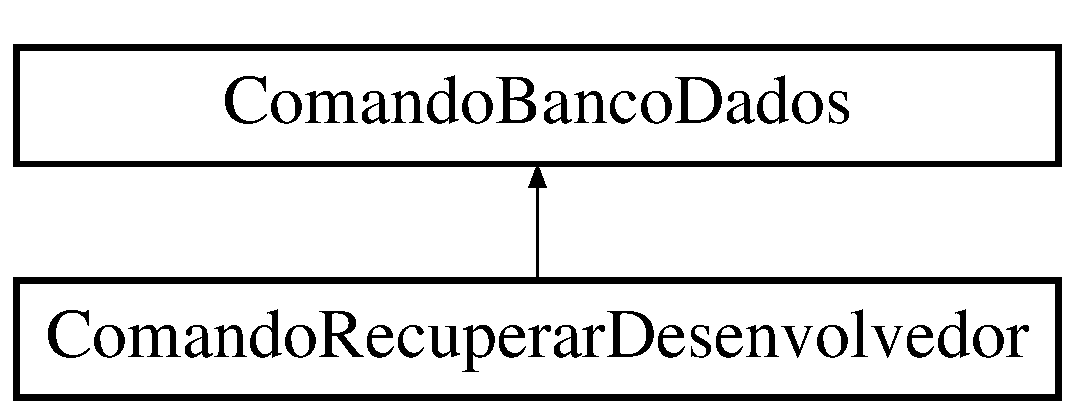
\includegraphics[height=2.000000cm]{class_comando_recuperar_desenvolvedor}
\end{center}
\end{figure}
\subsection*{Public Member Functions}
\begin{DoxyCompactItemize}
\item 
\hypertarget{class_comando_recuperar_desenvolvedor_ac42fbc8663e45bdad2988e9a8e636938}{}\label{class_comando_recuperar_desenvolvedor_ac42fbc8663e45bdad2988e9a8e636938} 
void {\bfseries executar} ()  throw (runtime\+\_\+error)
\end{DoxyCompactItemize}


\subsection{Detailed Description}
Classe responsável por\+: Recuperar desenvolvedor. 

Contém o protótipo do método responsável pelo comando do banco de dados, exclusivo do Gerente de \hyperlink{class_projeto}{Projeto}, de recuperar um desenvolvedor. 

The documentation for this class was generated from the following file\+:\begin{DoxyCompactItemize}
\item 
\hyperlink{_comandos_8h}{Comandos.\+h}\end{DoxyCompactItemize}

\hypertarget{class_comando_recuperar_gerente}{}\section{Comando\+Recuperar\+Gerente Class Reference}
\label{class_comando_recuperar_gerente}\index{Comando\+Recuperar\+Gerente@{Comando\+Recuperar\+Gerente}}


The documentation for this class was generated from the following file\+:\begin{DoxyCompactItemize}
\item 
\hyperlink{_lnegocio_8h}{Lnegocio.\+h}\end{DoxyCompactItemize}

\hypertarget{class_comando_recuperar_gerente_projeto}{}\section{Comando\+Recuperar\+Gerente\+Projeto Class Reference}
\label{class_comando_recuperar_gerente_projeto}\index{Comando\+Recuperar\+Gerente\+Projeto@{Comando\+Recuperar\+Gerente\+Projeto}}


Classe responsável por\+: Recuperar Gerente de projeto.  




{\ttfamily \#include $<$Comandos.\+h$>$}

Inheritance diagram for Comando\+Recuperar\+Gerente\+Projeto\+:\begin{figure}[H]
\begin{center}
\leavevmode
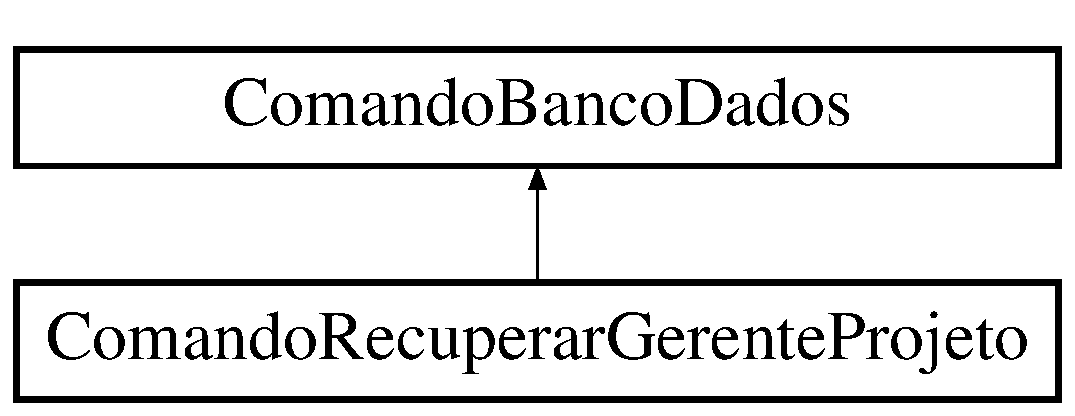
\includegraphics[height=2.000000cm]{class_comando_recuperar_gerente_projeto}
\end{center}
\end{figure}
\subsection*{Public Member Functions}
\begin{DoxyCompactItemize}
\item 
\hypertarget{class_comando_recuperar_gerente_projeto_a1c3b91e806c82dbfa8e606888a68f57e}{}\label{class_comando_recuperar_gerente_projeto_a1c3b91e806c82dbfa8e606888a68f57e} 
void {\bfseries executar} ()  throw (runtime\+\_\+error)
\end{DoxyCompactItemize}


\subsection{Detailed Description}
Classe responsável por\+: Recuperar Gerente de projeto. 

Contém o protótipo do método responsável pelo comando do banco de dados de recuperar um gerente de projeto. 

The documentation for this class was generated from the following file\+:\begin{DoxyCompactItemize}
\item 
\hyperlink{_comandos_8h}{Comandos.\+h}\end{DoxyCompactItemize}

\hypertarget{class_comando_recuperar_gerente_sistema}{}\section{Comando\+Recuperar\+Gerente\+Sistema Class Reference}
\label{class_comando_recuperar_gerente_sistema}\index{Comando\+Recuperar\+Gerente\+Sistema@{Comando\+Recuperar\+Gerente\+Sistema}}
Inheritance diagram for Comando\+Recuperar\+Gerente\+Sistema\+:\begin{figure}[H]
\begin{center}
\leavevmode
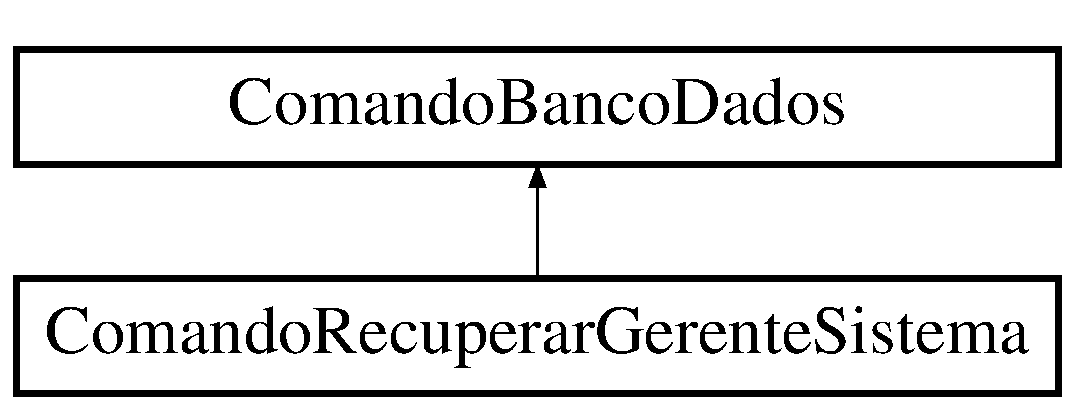
\includegraphics[height=2.000000cm]{class_comando_recuperar_gerente_sistema}
\end{center}
\end{figure}
\subsection*{Public Member Functions}
\begin{DoxyCompactItemize}
\item 
\hypertarget{class_comando_recuperar_gerente_sistema_af16a4d4b63f3fc691039b88fb1ffc156}{}\label{class_comando_recuperar_gerente_sistema_af16a4d4b63f3fc691039b88fb1ffc156} 
void {\bfseries executar} ()  throw (runtime\+\_\+error)
\end{DoxyCompactItemize}


The documentation for this class was generated from the following file\+:\begin{DoxyCompactItemize}
\item 
\hyperlink{_comandos_8h}{Comandos.\+h}\end{DoxyCompactItemize}

\hypertarget{class_comando_recuperar_projeto}{}\section{Comando\+Recuperar\+Projeto Class Reference}
\label{class_comando_recuperar_projeto}\index{Comando\+Recuperar\+Projeto@{Comando\+Recuperar\+Projeto}}


Classe responsável por\+: Recuperar projeto.  




{\ttfamily \#include $<$Comandos.\+h$>$}

Inheritance diagram for Comando\+Recuperar\+Projeto\+:\begin{figure}[H]
\begin{center}
\leavevmode
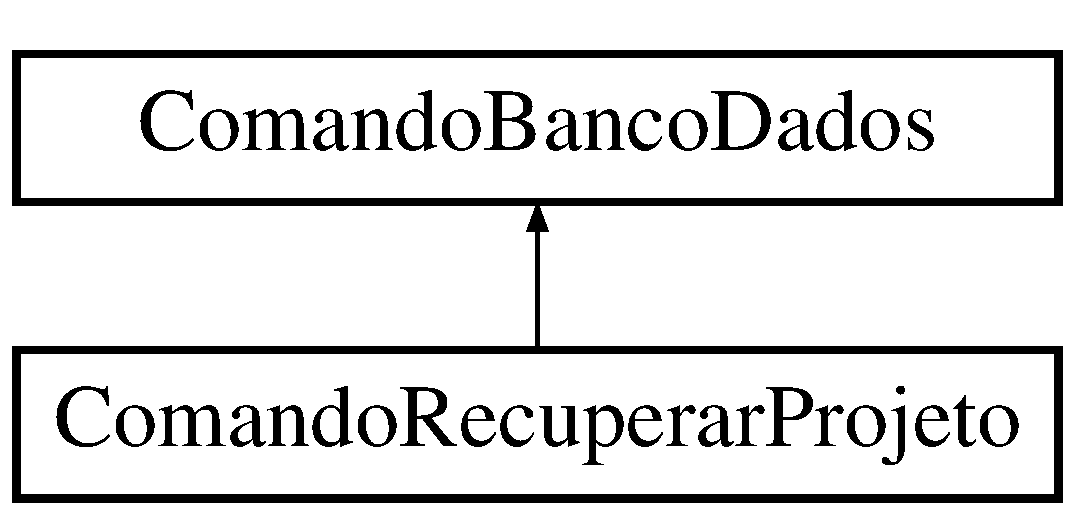
\includegraphics[height=2.000000cm]{class_comando_recuperar_projeto}
\end{center}
\end{figure}
\subsection*{Public Member Functions}
\begin{DoxyCompactItemize}
\item 
\hypertarget{class_comando_recuperar_projeto_af5deb7420caaacbaa84c8b9eed5239fa}{}\label{class_comando_recuperar_projeto_af5deb7420caaacbaa84c8b9eed5239fa} 
void {\bfseries executar} ()  throw (runtime\+\_\+error)
\end{DoxyCompactItemize}


\subsection{Detailed Description}
Classe responsável por\+: Recuperar projeto. 

Contém o protótipo do método responsável pelo comando do banco de dados, exclusivo do Gerente de \hyperlink{class_projeto}{Projeto}, de recuperar um projeto. 

The documentation for this class was generated from the following file\+:\begin{DoxyCompactItemize}
\item 
\hyperlink{_comandos_8h}{Comandos.\+h}\end{DoxyCompactItemize}

\hypertarget{class_comando_recuperar_sistema}{}\section{Comando\+Recuperar\+Sistema Class Reference}
\label{class_comando_recuperar_sistema}\index{Comando\+Recuperar\+Sistema@{Comando\+Recuperar\+Sistema}}


Classe responsável por\+: Recuperar Gerente de Sistema.  




{\ttfamily \#include $<$Comandos.\+h$>$}



\subsection{Detailed Description}
Classe responsável por\+: Recuperar Gerente de Sistema. 

Contém o protótipo do método responsável pelo comando do banco de dados de recuperar um gerente de sistema. 

The documentation for this class was generated from the following file\+:\begin{DoxyCompactItemize}
\item 
\hyperlink{_comandos_8h}{Comandos.\+h}\end{DoxyCompactItemize}

\hypertarget{class_comando_remover_desenvolvedor}{}\section{Comando\+Remover\+Desenvolvedor Class Reference}
\label{class_comando_remover_desenvolvedor}\index{Comando\+Remover\+Desenvolvedor@{Comando\+Remover\+Desenvolvedor}}


Classe responsável por\+: Remover desenvolvedor.  




{\ttfamily \#include $<$Comandos.\+h$>$}

Inheritance diagram for Comando\+Remover\+Desenvolvedor\+:\begin{figure}[H]
\begin{center}
\leavevmode
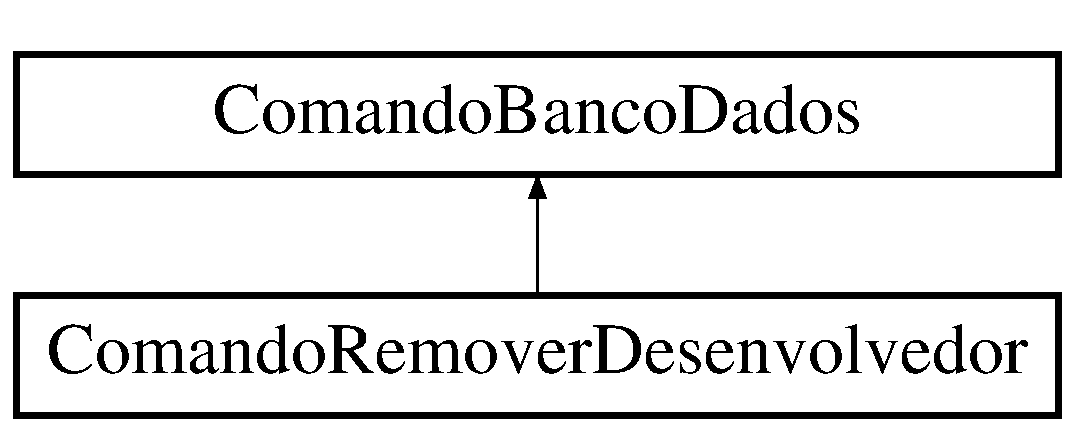
\includegraphics[height=2.000000cm]{class_comando_remover_desenvolvedor}
\end{center}
\end{figure}
\subsection*{Public Member Functions}
\begin{DoxyCompactItemize}
\item 
\hypertarget{class_comando_remover_desenvolvedor_a771c11514f5a1f892c007e8c34a049dc}{}\label{class_comando_remover_desenvolvedor_a771c11514f5a1f892c007e8c34a049dc} 
void {\bfseries executar} ()  throw (runtime\+\_\+error)
\end{DoxyCompactItemize}


\subsection{Detailed Description}
Classe responsável por\+: Remover desenvolvedor. 

Contém o protótipo do método responsável pelo comando do banco de dados, exclusivo do Gerente de \hyperlink{class_projeto}{Projeto}, de remover um desenvolvedor. 

The documentation for this class was generated from the following file\+:\begin{DoxyCompactItemize}
\item 
\hyperlink{_comandos_8h}{Comandos.\+h}\end{DoxyCompactItemize}

\hypertarget{class_comando_remover_gerente}{}\section{Comando\+Remover\+Gerente Class Reference}
\label{class_comando_remover_gerente}\index{Comando\+Remover\+Gerente@{Comando\+Remover\+Gerente}}


The documentation for this class was generated from the following file\+:\begin{DoxyCompactItemize}
\item 
\hyperlink{_lnegocio_8h}{Lnegocio.\+h}\end{DoxyCompactItemize}

\hypertarget{class_comando_remover_gerente_projeto}{}\section{Comando\+Remover\+Gerente\+Projeto Class Reference}
\label{class_comando_remover_gerente_projeto}\index{Comando\+Remover\+Gerente\+Projeto@{Comando\+Remover\+Gerente\+Projeto}}


Classe responsável por\+: Remover Gerente de projeto.  




{\ttfamily \#include $<$Comandos.\+h$>$}

Inheritance diagram for Comando\+Remover\+Gerente\+Projeto\+:\begin{figure}[H]
\begin{center}
\leavevmode
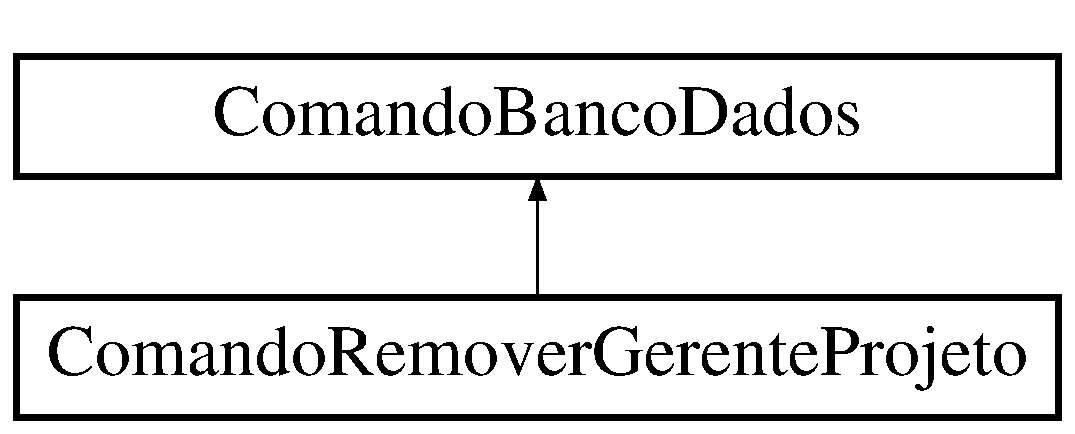
\includegraphics[height=2.000000cm]{class_comando_remover_gerente_projeto}
\end{center}
\end{figure}
\subsection*{Public Member Functions}
\begin{DoxyCompactItemize}
\item 
\hypertarget{class_comando_remover_gerente_projeto_adbced1ae3b1255f1e30793de1560c6ca}{}\label{class_comando_remover_gerente_projeto_adbced1ae3b1255f1e30793de1560c6ca} 
void {\bfseries executar} ()  throw (runtime\+\_\+error)
\end{DoxyCompactItemize}


\subsection{Detailed Description}
Classe responsável por\+: Remover Gerente de projeto. 

Contém o protótipo do método responsável pelo comando do banco de dados de remover um gerente de projeto. 

The documentation for this class was generated from the following file\+:\begin{DoxyCompactItemize}
\item 
\hyperlink{_comandos_8h}{Comandos.\+h}\end{DoxyCompactItemize}

\hypertarget{class_comando_remover_gerente_sistema}{}\section{Comando\+Remover\+Gerente\+Sistema Class Reference}
\label{class_comando_remover_gerente_sistema}\index{Comando\+Remover\+Gerente\+Sistema@{Comando\+Remover\+Gerente\+Sistema}}


Classe responsável por\+: Remover Gerente de sistema.  




{\ttfamily \#include $<$Comandos.\+h$>$}

Inheritance diagram for Comando\+Remover\+Gerente\+Sistema\+:\begin{figure}[H]
\begin{center}
\leavevmode
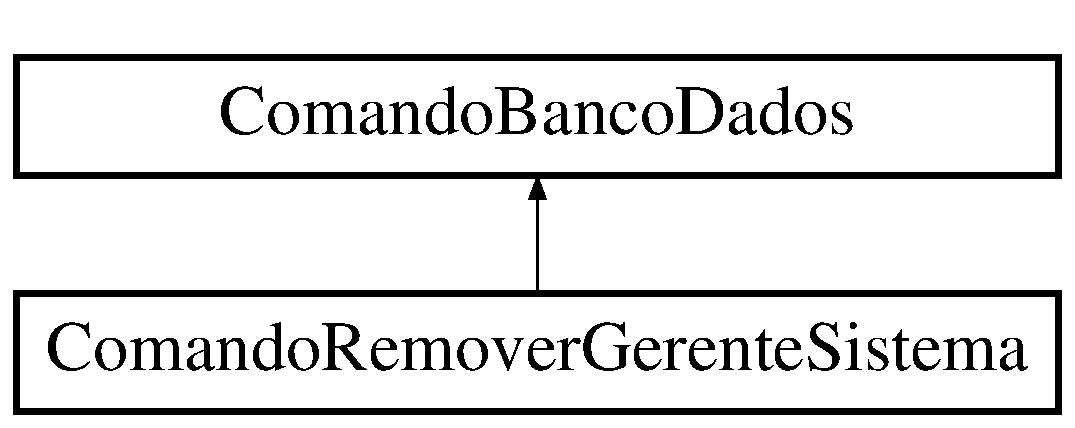
\includegraphics[height=2.000000cm]{class_comando_remover_gerente_sistema}
\end{center}
\end{figure}
\subsection*{Public Member Functions}
\begin{DoxyCompactItemize}
\item 
\hypertarget{class_comando_remover_gerente_sistema_a82299b1efa9133c3b0058a9d119445d0}{}\label{class_comando_remover_gerente_sistema_a82299b1efa9133c3b0058a9d119445d0} 
void {\bfseries executar} ()  throw (runtime\+\_\+error)
\end{DoxyCompactItemize}


\subsection{Detailed Description}
Classe responsável por\+: Remover Gerente de sistema. 

Contém o protótipo do método responsável pelo comando do banco de dados de remover um gerente de sistema. 

The documentation for this class was generated from the following file\+:\begin{DoxyCompactItemize}
\item 
\hyperlink{_comandos_8h}{Comandos.\+h}\end{DoxyCompactItemize}

\hypertarget{class_comando_remover_projeto}{}\section{Comando\+Remover\+Projeto Class Reference}
\label{class_comando_remover_projeto}\index{Comando\+Remover\+Projeto@{Comando\+Remover\+Projeto}}


Classe responsável por\+: Remover projeto.  




{\ttfamily \#include $<$Comandos.\+h$>$}

Inheritance diagram for Comando\+Remover\+Projeto\+:\begin{figure}[H]
\begin{center}
\leavevmode
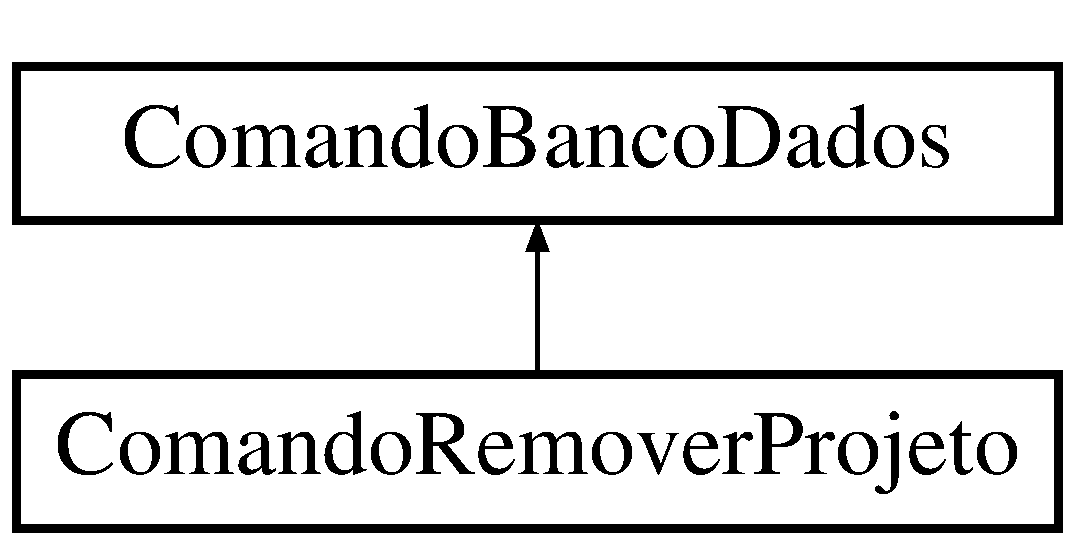
\includegraphics[height=2.000000cm]{class_comando_remover_projeto}
\end{center}
\end{figure}
\subsection*{Public Member Functions}
\begin{DoxyCompactItemize}
\item 
\hypertarget{class_comando_remover_projeto_a1eae6e7aa009522f481273874145b638}{}\label{class_comando_remover_projeto_a1eae6e7aa009522f481273874145b638} 
void {\bfseries executar} ()  throw (runtime\+\_\+error)
\end{DoxyCompactItemize}


\subsection{Detailed Description}
Classe responsável por\+: Remover projeto. 

Contém o protótipo do método responsável pelo comando do banco de dados, exclusivo do Gerente de \hyperlink{class_projeto}{Projeto}, de remover um projeto. 

The documentation for this class was generated from the following file\+:\begin{DoxyCompactItemize}
\item 
\hyperlink{_comandos_8h}{Comandos.\+h}\end{DoxyCompactItemize}

\hypertarget{class_custo}{}\section{Custo Class Reference}
\label{class_custo}\index{Custo@{Custo}}


Classe que cont�m os principais m�todos do custo do dominio.  




{\ttfamily \#include $<$Dominio.\+h$>$}

\subsection*{Public Member Functions}
\begin{DoxyCompactItemize}
\item 
\hypertarget{class_custo_a09c589d5456b2196458f8c443873e9a0}{}\label{class_custo_a09c589d5456b2196458f8c443873e9a0} 
{\bfseries Custo} (double)
\item 
\hypertarget{class_custo_a1bea1152f8aa5142d4d57aa0f533cb99}{}\label{class_custo_a1bea1152f8aa5142d4d57aa0f533cb99} 
void {\bfseries set\+Custo} (double)  throw (invalid\+\_\+argument)
\item 
\hypertarget{class_custo_a333904d06a8bb593a9fc97593deb3c5c}{}\label{class_custo_a333904d06a8bb593a9fc97593deb3c5c} 
double {\bfseries get\+Custo} () const
\item 
\hypertarget{class_custo_a79206173005fe355a7c191fac1f17c3f}{}\label{class_custo_a79206173005fe355a7c191fac1f17c3f} 
void {\bfseries is\+Custo\+Valid} (double)  throw (invalid\+\_\+argument)
\end{DoxyCompactItemize}


\subsection{Detailed Description}
Classe que cont�m os principais m�todos do custo do dominio. 

Cont�m os prot�tipos dos m�todos do nome referente ao dom�nio do sistema. 

The documentation for this class was generated from the following file\+:\begin{DoxyCompactItemize}
\item 
\hyperlink{_dominio_8h}{Dominio.\+h}\end{DoxyCompactItemize}

\hypertarget{class_data}{}\section{Data Class Reference}
\label{class_data}\index{Data@{Data}}


Classe que cont�m os principais m�todos da data do dominio.  




{\ttfamily \#include $<$Dominio.\+h$>$}

\subsection*{Public Member Functions}
\begin{DoxyCompactItemize}
\item 
\hypertarget{class_data_a7e546a6e6e55f93cb621011dff413f00}{}\label{class_data_a7e546a6e6e55f93cb621011dff413f00} 
{\bfseries Data} (string)
\item 
\hypertarget{class_data_a75a50f88bc966f20826a3959717a5acc}{}\label{class_data_a75a50f88bc966f20826a3959717a5acc} 
void {\bfseries set\+Data} (string)  throw (invalid\+\_\+argument)
\item 
\hypertarget{class_data_a13f25eafdc138d743e99eb4086d765a2}{}\label{class_data_a13f25eafdc138d743e99eb4086d765a2} 
string {\bfseries get\+Data} () const
\item 
\hypertarget{class_data_adb385e8096d959ea1e8901f223a0252d}{}\label{class_data_adb385e8096d959ea1e8901f223a0252d} 
void {\bfseries is\+Data\+Valid} (string)  throw (invalid\+\_\+argument)
\end{DoxyCompactItemize}


\subsection{Detailed Description}
Classe que cont�m os principais m�todos da data do dominio. 

Cont�m os prot�tipos dos m�todos do nome referente ao dom�nio do sistema. 

The documentation for this class was generated from the following file\+:\begin{DoxyCompactItemize}
\item 
\hyperlink{_dominio_8h}{Dominio.\+h}\end{DoxyCompactItemize}

\hypertarget{class_desenvolvedor}{}\section{Desenvolvedor Class Reference}
\label{class_desenvolvedor}\index{Desenvolvedor@{Desenvolvedor}}


Classe que cont�m os principais m�todos da entidade de desenvolvedor.  




{\ttfamily \#include $<$Entidade.\+h$>$}

Inheritance diagram for Desenvolvedor\+:\begin{figure}[H]
\begin{center}
\leavevmode
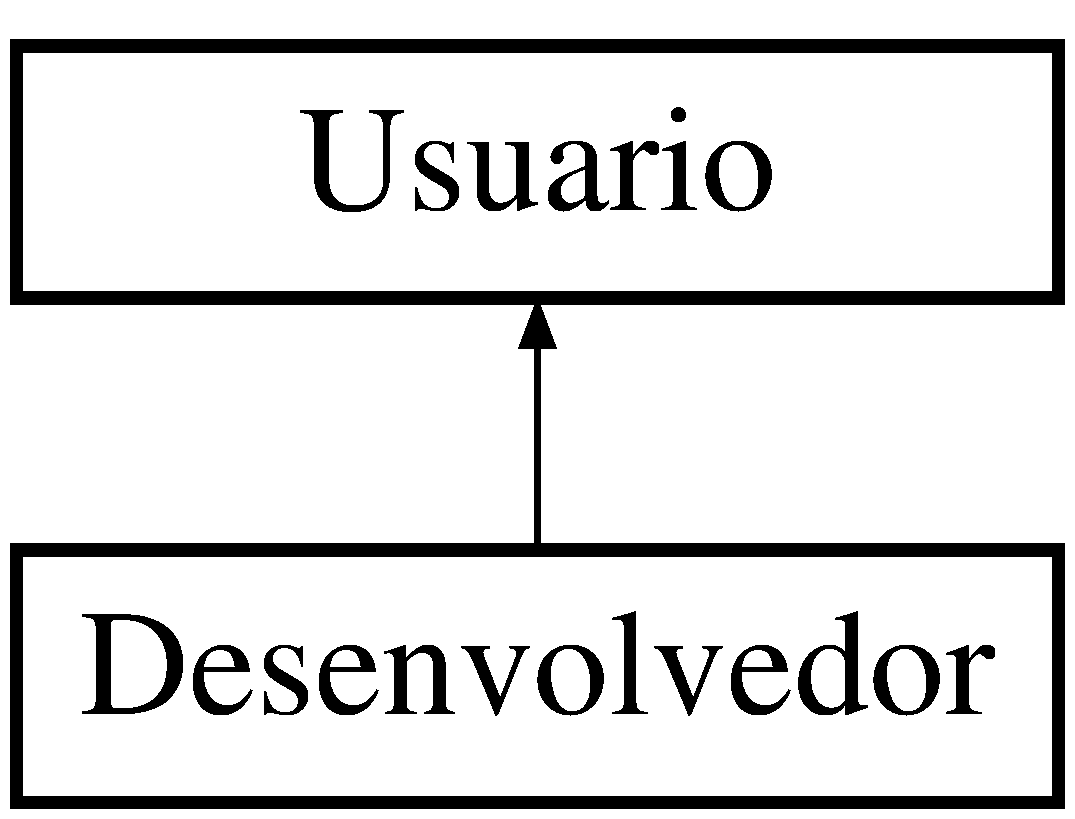
\includegraphics[height=2.000000cm]{class_desenvolvedor}
\end{center}
\end{figure}
\subsection*{Public Attributes}
\begin{DoxyCompactItemize}
\item 
\hypertarget{class_desenvolvedor_af2a613f35fc24cbbb07cfea389147035}{}\label{class_desenvolvedor_af2a613f35fc24cbbb07cfea389147035} 
\hyperlink{class_funcao}{Funcao} {\bfseries subfuncao}
\item 
\hypertarget{class_desenvolvedor_a14240293f926b2e560496cc2da2498e3}{}\label{class_desenvolvedor_a14240293f926b2e560496cc2da2498e3} 
\hyperlink{class_email}{Email} {\bfseries email}
\end{DoxyCompactItemize}
\subsection*{Additional Inherited Members}


\subsection{Detailed Description}
Classe que cont�m os principais m�todos da entidade de desenvolvedor. 

Cont�m os prot�tipos dos m�todos da classe desenvolvedor referente �s entidades do sistema. 

The documentation for this class was generated from the following file\+:\begin{DoxyCompactItemize}
\item 
\hyperlink{_entidade_8h}{Entidade.\+h}\end{DoxyCompactItemize}

\hypertarget{class_email}{}\section{Email Class Reference}
\label{class_email}\index{Email@{Email}}


Classe que cont�m os principais m�todos do email do dominio.  




{\ttfamily \#include $<$Dominio.\+h$>$}

\subsection*{Public Member Functions}
\begin{DoxyCompactItemize}
\item 
\hypertarget{class_email_abfa7891fe9bc84c6f19e91a7fceb2fed}{}\label{class_email_abfa7891fe9bc84c6f19e91a7fceb2fed} 
{\bfseries Email} (string)
\item 
\hypertarget{class_email_a47fc9d4d76a2e2a7bc502f16c1d034be}{}\label{class_email_a47fc9d4d76a2e2a7bc502f16c1d034be} 
void {\bfseries set\+Email} (string)  throw (invalid\+\_\+argument)
\item 
\hypertarget{class_email_a6c314589c2042bf2234a9b5781d50def}{}\label{class_email_a6c314589c2042bf2234a9b5781d50def} 
string {\bfseries get\+Email} () const
\item 
\hypertarget{class_email_a3f34ee2a29394ccfe2ab3f41a9461deb}{}\label{class_email_a3f34ee2a29394ccfe2ab3f41a9461deb} 
void {\bfseries is\+Email\+Valid} (string)  throw (invalid\+\_\+argument)
\end{DoxyCompactItemize}


\subsection{Detailed Description}
Classe que cont�m os principais m�todos do email do dominio. 

Cont�m os prot�tipos dos m�todos do nome referente ao dom�nio do sistema. 

The documentation for this class was generated from the following file\+:\begin{DoxyCompactItemize}
\item 
\hyperlink{_dominio_8h}{Dominio.\+h}\end{DoxyCompactItemize}

\hypertarget{class_estado_projeto}{}\section{Estado\+Projeto Class Reference}
\label{class_estado_projeto}\index{Estado\+Projeto@{Estado\+Projeto}}


Classe que cont�m os principais m�todos do Estado do \hyperlink{class_projeto}{Projeto} do dominio.  




{\ttfamily \#include $<$Dominio.\+h$>$}

\subsection*{Public Member Functions}
\begin{DoxyCompactItemize}
\item 
\hypertarget{class_estado_projeto_a7be713cc5b033e1bba38ef4483506d73}{}\label{class_estado_projeto_a7be713cc5b033e1bba38ef4483506d73} 
{\bfseries Estado\+Projeto} (int)
\item 
\hypertarget{class_estado_projeto_a06a83964d60cd90169e17d549f6341d3}{}\label{class_estado_projeto_a06a83964d60cd90169e17d549f6341d3} 
void {\bfseries set\+Estado\+Projeto} (int)  throw (invalid\+\_\+argument)
\item 
\hypertarget{class_estado_projeto_a7580373c21f8741e6b09b50d14881306}{}\label{class_estado_projeto_a7580373c21f8741e6b09b50d14881306} 
int {\bfseries get\+Estado\+Projeto} () const
\item 
\hypertarget{class_estado_projeto_a9435e519b628685c4c7b8ba6032efca6}{}\label{class_estado_projeto_a9435e519b628685c4c7b8ba6032efca6} 
void {\bfseries is\+Estado\+Projeto\+Valid} (int)  throw (invalid\+\_\+argument)
\end{DoxyCompactItemize}


\subsection{Detailed Description}
Classe que cont�m os principais m�todos do Estado do \hyperlink{class_projeto}{Projeto} do dominio. 

Cont�m os prot�tipos dos m�todos do nome referente ao dom�nio do sistema. 

The documentation for this class was generated from the following file\+:\begin{DoxyCompactItemize}
\item 
\hyperlink{_dominio_8h}{Dominio.\+h}\end{DoxyCompactItemize}

\hypertarget{class_fase}{}\section{Fase Class Reference}
\label{class_fase}\index{Fase@{Fase}}


Classe que cont�m os principais m�todos da fase do dominio.  




{\ttfamily \#include $<$Dominio.\+h$>$}

\subsection*{Public Member Functions}
\begin{DoxyCompactItemize}
\item 
\hypertarget{class_fase_a5d73915ccac38d45f41c5c8431e795bf}{}\label{class_fase_a5d73915ccac38d45f41c5c8431e795bf} 
{\bfseries Fase} (int)
\item 
\hypertarget{class_fase_a8aee22de0f7c37314446816aee867873}{}\label{class_fase_a8aee22de0f7c37314446816aee867873} 
void {\bfseries set\+Fase} (int)  throw (invalid\+\_\+argument)
\item 
\hypertarget{class_fase_a506a7b6870de5e05a94a240ceb426aca}{}\label{class_fase_a506a7b6870de5e05a94a240ceb426aca} 
int {\bfseries get\+Fase} () const
\item 
\hypertarget{class_fase_a745b7ec35600766acf12049691732eb8}{}\label{class_fase_a745b7ec35600766acf12049691732eb8} 
void {\bfseries is\+Fase\+Valid} (int)  throw (invalid\+\_\+argument)
\end{DoxyCompactItemize}


\subsection{Detailed Description}
Classe que cont�m os principais m�todos da fase do dominio. 

Cont�m os prot�tipos dos m�todos do nome referente ao dom�nio do sistema. 

The documentation for this class was generated from the following file\+:\begin{DoxyCompactItemize}
\item 
\hyperlink{_dominio_8h}{Dominio.\+h}\end{DoxyCompactItemize}

\hypertarget{class_fase_projeto}{}\section{Fase\+Projeto Class Reference}
\label{class_fase_projeto}\index{Fase\+Projeto@{Fase\+Projeto}}


Classe que cont�m os principais m�todos da entidade de fase de projeto.  




{\ttfamily \#include $<$Entidade.\+h$>$}

\subsection*{Public Attributes}
\begin{DoxyCompactItemize}
\item 
\hypertarget{class_fase_projeto_a8e0053fc1257ac01370603d867143f77}{}\label{class_fase_projeto_a8e0053fc1257ac01370603d867143f77} 
\hyperlink{class_fase}{Fase} {\bfseries fase}
\item 
\hypertarget{class_fase_projeto_a2aa6721fefd89944a6e12aefc46610dd}{}\label{class_fase_projeto_a2aa6721fefd89944a6e12aefc46610dd} 
\hyperlink{class_data}{Data} {\bfseries data\+Inicio}
\item 
\hypertarget{class_fase_projeto_a20e463c1f4ce962eff03698b58dedac5}{}\label{class_fase_projeto_a20e463c1f4ce962eff03698b58dedac5} 
\hyperlink{class_data}{Data} {\bfseries data\+Fim}
\end{DoxyCompactItemize}


\subsection{Detailed Description}
Classe que cont�m os principais m�todos da entidade de fase de projeto. 

Cont�m os prot�tipos dos m�todos da classe fase de projeto referente �s entidades do sistema. 

The documentation for this class was generated from the following file\+:\begin{DoxyCompactItemize}
\item 
\hyperlink{_entidade_8h}{Entidade.\+h}\end{DoxyCompactItemize}

\hypertarget{class_funcao}{}\section{Funcao Class Reference}
\label{class_funcao}\index{Funcao@{Funcao}}


Classe que cont�m os principais m�todos da fun��o do dominio.  




{\ttfamily \#include $<$Dominio.\+h$>$}

\subsection*{Public Member Functions}
\begin{DoxyCompactItemize}
\item 
\hypertarget{class_funcao_a7d9d695b57316586b1a44320012ed1d9}{}\label{class_funcao_a7d9d695b57316586b1a44320012ed1d9} 
{\bfseries Funcao} (int)
\item 
\hypertarget{class_funcao_a530bf1a4e7a4a868c586fe5385d54c26}{}\label{class_funcao_a530bf1a4e7a4a868c586fe5385d54c26} 
void {\bfseries set\+Funcao} (int)  throw (invalid\+\_\+argument)
\item 
\hypertarget{class_funcao_ad6ecc462b997bc713436045762c6c7da}{}\label{class_funcao_ad6ecc462b997bc713436045762c6c7da} 
int {\bfseries get\+Funcao} () const
\item 
\hypertarget{class_funcao_aed416b4dd3ef2d4fdc1b5d38285da422}{}\label{class_funcao_aed416b4dd3ef2d4fdc1b5d38285da422} 
void {\bfseries is\+Funcao\+Valid} (int)  throw (invalid\+\_\+argument)
\end{DoxyCompactItemize}


\subsection{Detailed Description}
Classe que cont�m os principais m�todos da fun��o do dominio. 

Cont�m os prot�tipos dos m�todos do nome referente ao dom�nio do sistema. 

The documentation for this class was generated from the following file\+:\begin{DoxyCompactItemize}
\item 
\hyperlink{_dominio_8h}{Dominio.\+h}\end{DoxyCompactItemize}

\hypertarget{class_gerente_projeto}{}\section{Gerente\+Projeto Class Reference}
\label{class_gerente_projeto}\index{Gerente\+Projeto@{Gerente\+Projeto}}


Classe que cont�m os principais m�todos da entidade de gerente de projeto.  




{\ttfamily \#include $<$Entidade.\+h$>$}

Inheritance diagram for Gerente\+Projeto\+:\begin{figure}[H]
\begin{center}
\leavevmode
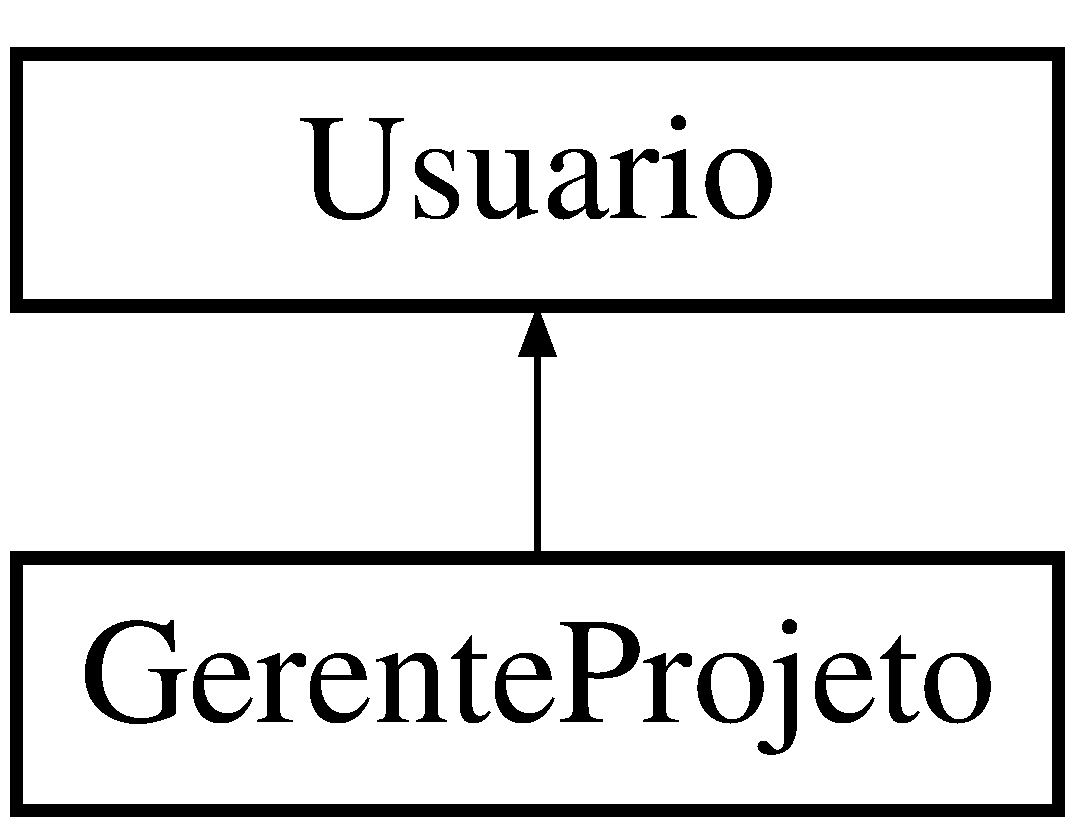
\includegraphics[height=2.000000cm]{class_gerente_projeto}
\end{center}
\end{figure}
\subsection*{Public Attributes}
\begin{DoxyCompactItemize}
\item 
\hypertarget{class_gerente_projeto_a3f0c9ac2da10a480a4502acfe321d6e9}{}\label{class_gerente_projeto_a3f0c9ac2da10a480a4502acfe321d6e9} 
\hyperlink{class_telefone}{Telefone} {\bfseries telefone}
\end{DoxyCompactItemize}
\subsection*{Additional Inherited Members}


\subsection{Detailed Description}
Classe que cont�m os principais m�todos da entidade de gerente de projeto. 

Cont�m os prot�tipos dos m�todos da classe gerente de projeto referente �s entidades do sistema. 

The documentation for this class was generated from the following file\+:\begin{DoxyCompactItemize}
\item 
\hyperlink{_entidade_8h}{Entidade.\+h}\end{DoxyCompactItemize}

\hypertarget{class_gerente_sistema}{}\section{Gerente\+Sistema Class Reference}
\label{class_gerente_sistema}\index{Gerente\+Sistema@{Gerente\+Sistema}}


Classe que cont�m os principais m�todos da entidade de gerente de sistema.  




{\ttfamily \#include $<$Entidade.\+h$>$}

Inheritance diagram for Gerente\+Sistema\+:\begin{figure}[H]
\begin{center}
\leavevmode
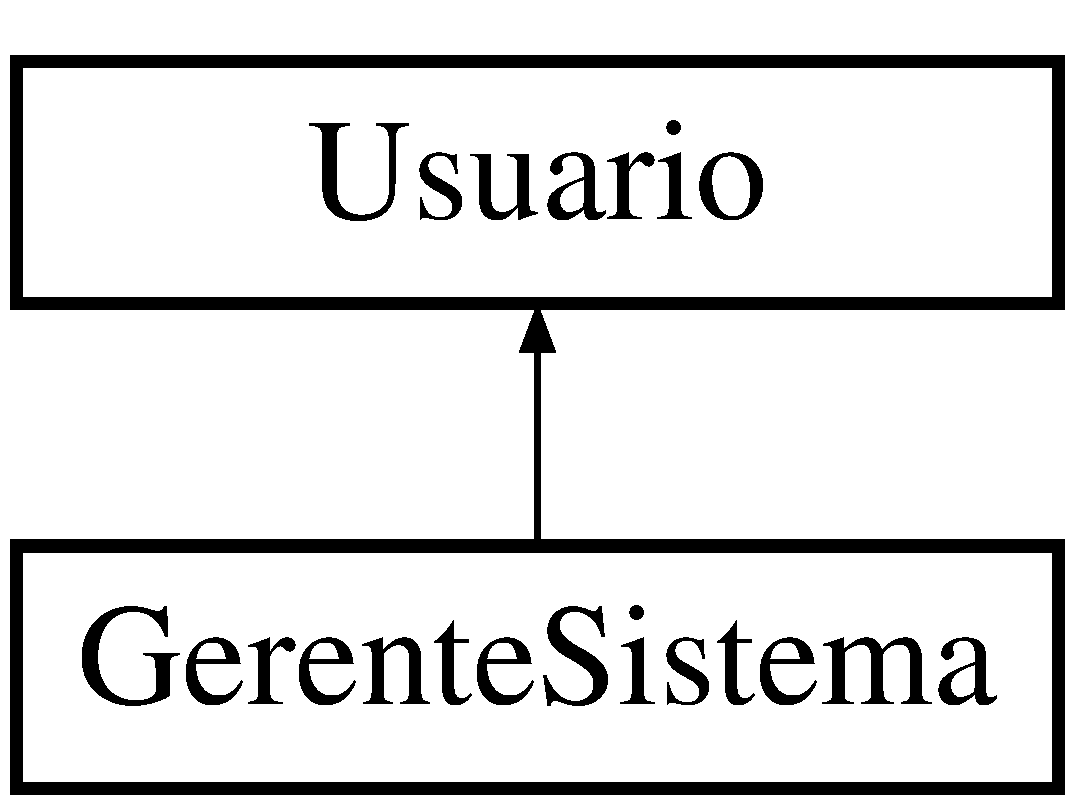
\includegraphics[height=2.000000cm]{class_gerente_sistema}
\end{center}
\end{figure}
\subsection*{Additional Inherited Members}


\subsection{Detailed Description}
Classe que cont�m os principais m�todos da entidade de gerente de sistema. 

Cont�m os prot�tipos dos m�todos da classe gerente de sistema referente �s entidades do sistema. 

The documentation for this class was generated from the following file\+:\begin{DoxyCompactItemize}
\item 
\hyperlink{_entidade_8h}{Entidade.\+h}\end{DoxyCompactItemize}

\hypertarget{class_i_l_n_autenticacao}{}\section{I\+L\+N\+Autenticacao Class Reference}
\label{class_i_l_n_autenticacao}\index{I\+L\+N\+Autenticacao@{I\+L\+N\+Autenticacao}}


Classe que contém os principais métodos dos comandos de autenticação da interface de negocio.  




{\ttfamily \#include $<$Interfaces.\+h$>$}

Inheritance diagram for I\+L\+N\+Autenticacao\+:\begin{figure}[H]
\begin{center}
\leavevmode
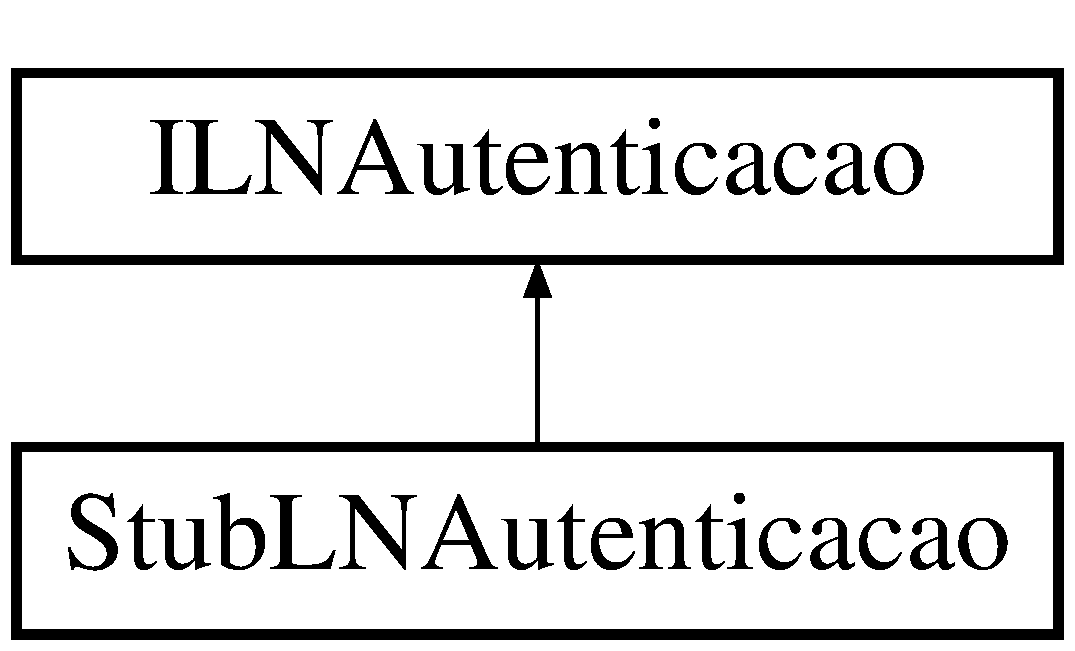
\includegraphics[height=2.000000cm]{class_i_l_n_autenticacao}
\end{center}
\end{figure}
\subsection*{Public Member Functions}
\begin{DoxyCompactItemize}
\item 
\hypertarget{class_i_l_n_autenticacao_ac73f153e0e417aaf5cd07fe497d74f87}{}\label{class_i_l_n_autenticacao_ac73f153e0e417aaf5cd07fe497d74f87} 
virtual \hyperlink{class_resultado_autenticacao}{Resultado\+Autenticacao} {\bfseries autenticar} (const \hyperlink{class_matricula}{Matricula} \&, const \hyperlink{class_senha}{Senha} \&)=0  throw (runtime\+\_\+error)
\end{DoxyCompactItemize}


\subsection{Detailed Description}
Classe que contém os principais métodos dos comandos de autenticação da interface de negocio. 

Contém os protótipos dos métodos utilizados que se comunicam com a interface de negocio. 

The documentation for this class was generated from the following file\+:\begin{DoxyCompactItemize}
\item 
\hyperlink{_interfaces_8h}{Interfaces.\+h}\end{DoxyCompactItemize}

\hypertarget{class_i_l_n_desenvolvedor}{}\section{I\+L\+N\+Desenvolvedor Class Reference}
\label{class_i_l_n_desenvolvedor}\index{I\+L\+N\+Desenvolvedor@{I\+L\+N\+Desenvolvedor}}


Classe que contém os principais métodos dos comandos de desenvolvedor da interface de negocio.  




{\ttfamily \#include $<$Interfaces.\+h$>$}

Inheritance diagram for I\+L\+N\+Desenvolvedor\+:\begin{figure}[H]
\begin{center}
\leavevmode
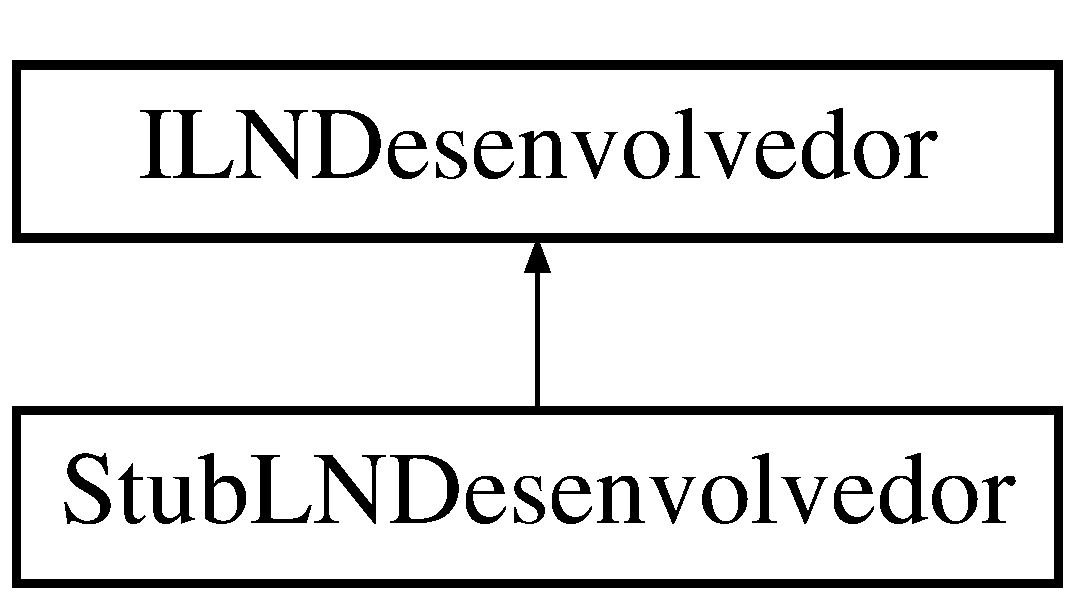
\includegraphics[height=2.000000cm]{class_i_l_n_desenvolvedor}
\end{center}
\end{figure}
\subsection*{Public Member Functions}
\begin{DoxyCompactItemize}
\item 
\hypertarget{class_i_l_n_desenvolvedor_a336a4fd765096259da80e8c92a89b7bb}{}\label{class_i_l_n_desenvolvedor_a336a4fd765096259da80e8c92a89b7bb} 
virtual \hyperlink{class_resultado_desenvolvedor}{Resultado\+Desenvolvedor} {\bfseries incluir} (const \hyperlink{class_desenvolvedor}{Desenvolvedor} \&)=0  throw (runtime\+\_\+error)
\item 
\hypertarget{class_i_l_n_desenvolvedor_abc06df16cebd8e870bc3cdc99a315427}{}\label{class_i_l_n_desenvolvedor_abc06df16cebd8e870bc3cdc99a315427} 
virtual \hyperlink{class_resultado_desenvolvedor}{Resultado\+Desenvolvedor} {\bfseries remover} (const \hyperlink{class_matricula}{Matricula} \&)=0  throw (runtime\+\_\+error)
\item 
\hypertarget{class_i_l_n_desenvolvedor_aa53b2f33420e8747b6c01e938aa3a6c6}{}\label{class_i_l_n_desenvolvedor_aa53b2f33420e8747b6c01e938aa3a6c6} 
virtual \hyperlink{class_resultado_desenvolvedor}{Resultado\+Desenvolvedor} {\bfseries pesquisar} (const \hyperlink{class_matricula}{Matricula} \&)=0  throw (runtime\+\_\+error)
\item 
\hypertarget{class_i_l_n_desenvolvedor_aeb0d5d1e8a46d3d739b5059eb9978868}{}\label{class_i_l_n_desenvolvedor_aeb0d5d1e8a46d3d739b5059eb9978868} 
virtual \hyperlink{class_resultado_desenvolvedor}{Resultado\+Desenvolvedor} {\bfseries editar} (const \hyperlink{class_desenvolvedor}{Desenvolvedor} \&)=0  throw (runtime\+\_\+error)
\end{DoxyCompactItemize}


\subsection{Detailed Description}
Classe que contém os principais métodos dos comandos de desenvolvedor da interface de negocio. 

Contém os protótipos dos métodos utilizados que se comunicam com a interface de negocio. 

The documentation for this class was generated from the following file\+:\begin{DoxyCompactItemize}
\item 
\hyperlink{_interfaces_8h}{Interfaces.\+h}\end{DoxyCompactItemize}

\hypertarget{class_i_l_n_gerente_projeto}{}\section{I\+L\+N\+Gerente\+Projeto Class Reference}
\label{class_i_l_n_gerente_projeto}\index{I\+L\+N\+Gerente\+Projeto@{I\+L\+N\+Gerente\+Projeto}}


Classe que contém os principais métodos dos comandos de gerente de projetos da interface de negocio.  




{\ttfamily \#include $<$Interfaces.\+h$>$}

Inheritance diagram for I\+L\+N\+Gerente\+Projeto\+:\begin{figure}[H]
\begin{center}
\leavevmode
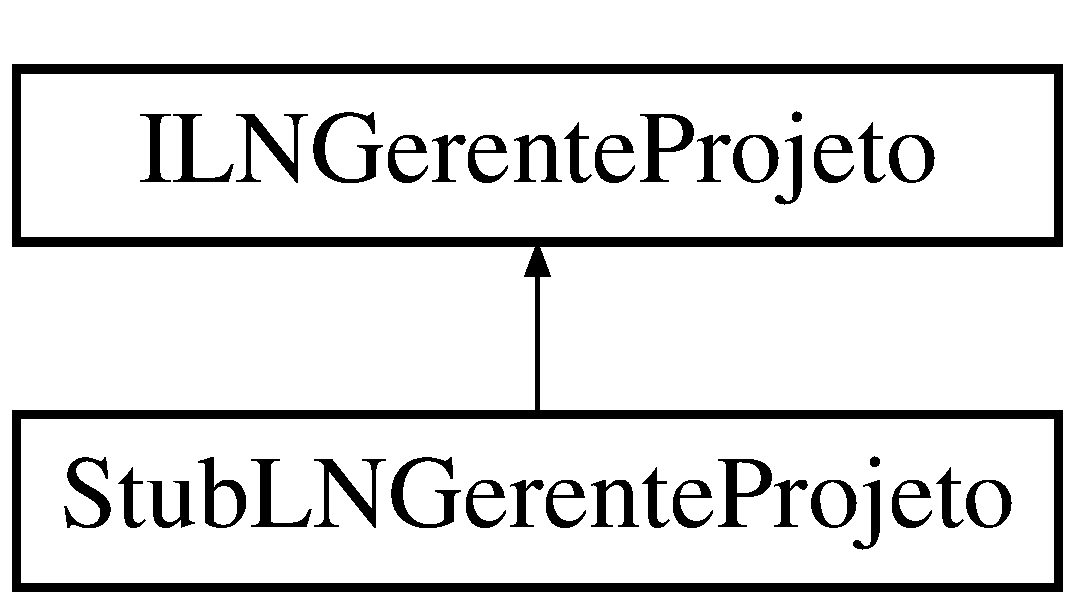
\includegraphics[height=2.000000cm]{class_i_l_n_gerente_projeto}
\end{center}
\end{figure}
\subsection*{Public Member Functions}
\begin{DoxyCompactItemize}
\item 
\hypertarget{class_i_l_n_gerente_projeto_ac27caf6424cdbd188cb7e1c985d0e3a3}{}\label{class_i_l_n_gerente_projeto_ac27caf6424cdbd188cb7e1c985d0e3a3} 
virtual \hyperlink{class_resultado_gerente_projeto}{Resultado\+Gerente\+Projeto} {\bfseries incluir} (const \hyperlink{class_gerente_projeto}{Gerente\+Projeto} \&)=0  throw (runtime\+\_\+error)
\item 
\hypertarget{class_i_l_n_gerente_projeto_ad8c71f1aba202c932543bc9712f4d478}{}\label{class_i_l_n_gerente_projeto_ad8c71f1aba202c932543bc9712f4d478} 
virtual \hyperlink{class_resultado_gerente_projeto}{Resultado\+Gerente\+Projeto} {\bfseries remover} (const \hyperlink{class_matricula}{Matricula} \&)=0  throw (runtime\+\_\+error)
\item 
\hypertarget{class_i_l_n_gerente_projeto_a488643773ff8a07926a27e70005e6607}{}\label{class_i_l_n_gerente_projeto_a488643773ff8a07926a27e70005e6607} 
virtual \hyperlink{class_resultado_gerente_projeto}{Resultado\+Gerente\+Projeto} {\bfseries pesquisar} (const \hyperlink{class_matricula}{Matricula} \&)=0  throw (runtime\+\_\+error)
\item 
\hypertarget{class_i_l_n_gerente_projeto_a9aa856e1d83880b5022315f08152bc68}{}\label{class_i_l_n_gerente_projeto_a9aa856e1d83880b5022315f08152bc68} 
virtual \hyperlink{class_resultado_gerente_projeto}{Resultado\+Gerente\+Projeto} {\bfseries editar} (const \hyperlink{class_gerente_projeto}{Gerente\+Projeto} \&)=0  throw (runtime\+\_\+error)
\end{DoxyCompactItemize}


\subsection{Detailed Description}
Classe que contém os principais métodos dos comandos de gerente de projetos da interface de negocio. 

Contém os protótipos dos métodos utilizados que se comunicam com a interface de negocio. 

The documentation for this class was generated from the following file\+:\begin{DoxyCompactItemize}
\item 
\hyperlink{_interfaces_8h}{Interfaces.\+h}\end{DoxyCompactItemize}

\hypertarget{class_i_l_n_gerente_sistema}{}\section{I\+L\+N\+Gerente\+Sistema Class Reference}
\label{class_i_l_n_gerente_sistema}\index{I\+L\+N\+Gerente\+Sistema@{I\+L\+N\+Gerente\+Sistema}}


Classe que contém os principais métodos dos comandos de gerente de sistema da interface de negocio.  




{\ttfamily \#include $<$Interfaces.\+h$>$}

Inheritance diagram for I\+L\+N\+Gerente\+Sistema\+:\begin{figure}[H]
\begin{center}
\leavevmode
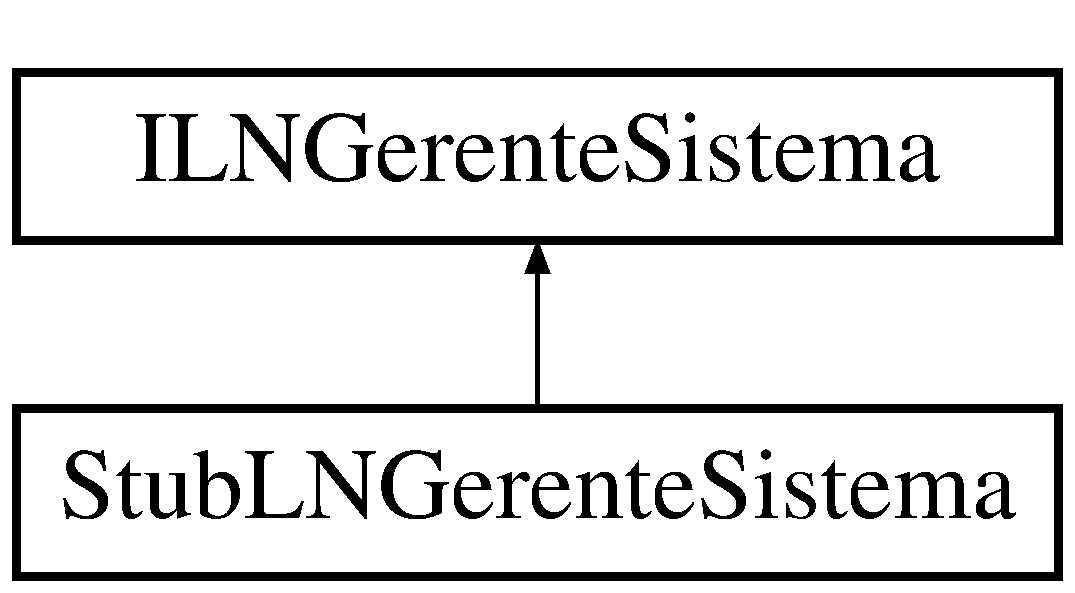
\includegraphics[height=2.000000cm]{class_i_l_n_gerente_sistema}
\end{center}
\end{figure}
\subsection*{Public Member Functions}
\begin{DoxyCompactItemize}
\item 
\hypertarget{class_i_l_n_gerente_sistema_a2e8119e31d7288816a77660b7e6bf514}{}\label{class_i_l_n_gerente_sistema_a2e8119e31d7288816a77660b7e6bf514} 
virtual \hyperlink{class_resultado_gerente_sistema}{Resultado\+Gerente\+Sistema} {\bfseries incluir} (const \hyperlink{class_gerente_sistema}{Gerente\+Sistema} \&)=0  throw (runtime\+\_\+error)
\item 
\hypertarget{class_i_l_n_gerente_sistema_a9c3b27feb0b9e041988e4406332f0680}{}\label{class_i_l_n_gerente_sistema_a9c3b27feb0b9e041988e4406332f0680} 
virtual \hyperlink{class_resultado_gerente_sistema}{Resultado\+Gerente\+Sistema} {\bfseries remover} (const \hyperlink{class_matricula}{Matricula} \&)=0  throw (runtime\+\_\+error)
\item 
\hypertarget{class_i_l_n_gerente_sistema_a91d12c41e8bce59edaf38d857dd6c3b6}{}\label{class_i_l_n_gerente_sistema_a91d12c41e8bce59edaf38d857dd6c3b6} 
virtual \hyperlink{class_resultado_gerente_sistema}{Resultado\+Gerente\+Sistema} {\bfseries pesquisar} (const \hyperlink{class_matricula}{Matricula} \&)=0  throw (runtime\+\_\+error)
\item 
\hypertarget{class_i_l_n_gerente_sistema_a5653ec6bc3c34de3455a5566ec12759c}{}\label{class_i_l_n_gerente_sistema_a5653ec6bc3c34de3455a5566ec12759c} 
virtual \hyperlink{class_resultado_gerente_sistema}{Resultado\+Gerente\+Sistema} {\bfseries editar} (const \hyperlink{class_gerente_sistema}{Gerente\+Sistema} \&)=0  throw (runtime\+\_\+error)
\end{DoxyCompactItemize}


\subsection{Detailed Description}
Classe que contém os principais métodos dos comandos de gerente de sistema da interface de negocio. 

Contém os protótipos dos métodos utilizados que se comunicam com a interface de negocio. 

The documentation for this class was generated from the following file\+:\begin{DoxyCompactItemize}
\item 
\hyperlink{_interfaces_8h}{Interfaces.\+h}\end{DoxyCompactItemize}

\hypertarget{class_i_l_n_projeto}{}\section{I\+L\+N\+Projeto Class Reference}
\label{class_i_l_n_projeto}\index{I\+L\+N\+Projeto@{I\+L\+N\+Projeto}}


Classe que contém os principais métodos dos comandos de projeto da interface de negocio.  




{\ttfamily \#include $<$Interfaces.\+h$>$}

Inheritance diagram for I\+L\+N\+Projeto\+:\begin{figure}[H]
\begin{center}
\leavevmode
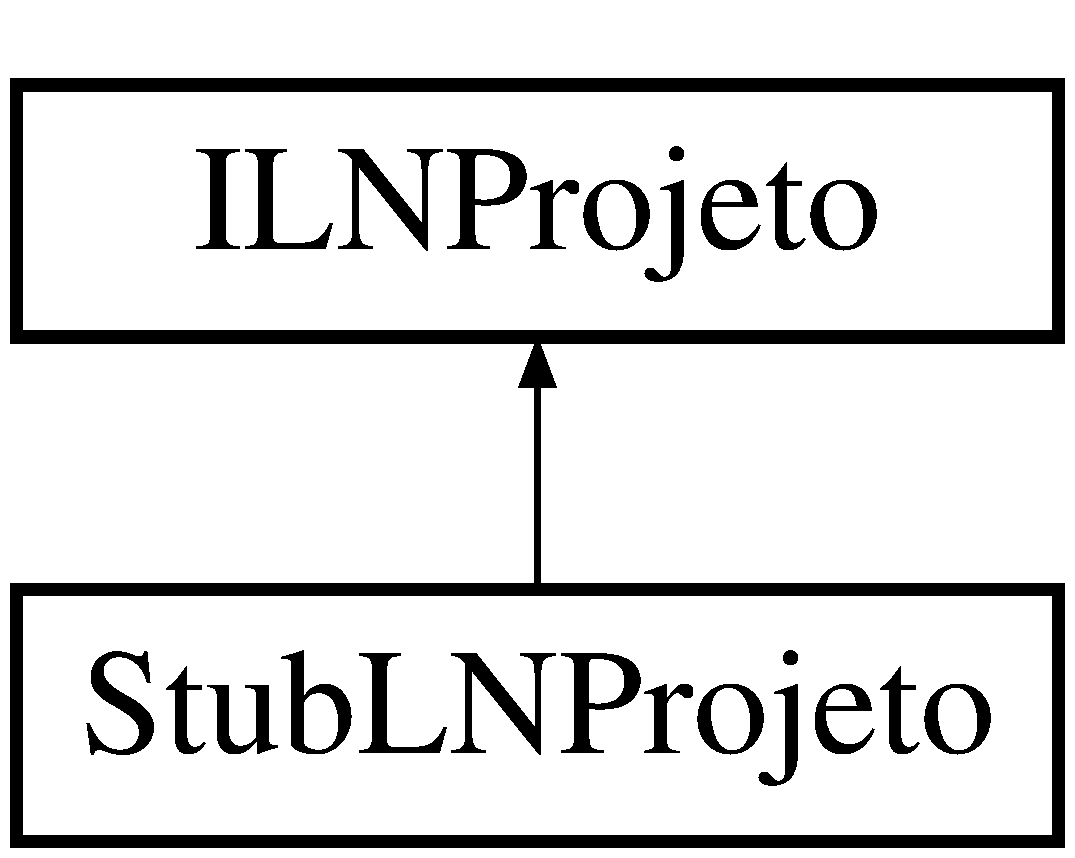
\includegraphics[height=2.000000cm]{class_i_l_n_projeto}
\end{center}
\end{figure}
\subsection*{Public Member Functions}
\begin{DoxyCompactItemize}
\item 
\hypertarget{class_i_l_n_projeto_a6b97553e8adf3ec40fcb1de1da64cac1}{}\label{class_i_l_n_projeto_a6b97553e8adf3ec40fcb1de1da64cac1} 
virtual \hyperlink{class_resultado_projeto}{Resultado\+Projeto} {\bfseries incluir} (const \hyperlink{class_projeto}{Projeto} \&)=0  throw (runtime\+\_\+error)
\item 
\hypertarget{class_i_l_n_projeto_af30c088be5531dc06966b3a8d0ff06ed}{}\label{class_i_l_n_projeto_af30c088be5531dc06966b3a8d0ff06ed} 
virtual \hyperlink{class_resultado_projeto}{Resultado\+Projeto} {\bfseries remover} (const \hyperlink{class_codigo_projeto}{Codigo\+Projeto} \&)=0  throw (runtime\+\_\+error)
\item 
\hypertarget{class_i_l_n_projeto_ad656d7f8a4f62281b561b69b5e59e914}{}\label{class_i_l_n_projeto_ad656d7f8a4f62281b561b69b5e59e914} 
virtual \hyperlink{class_resultado_projeto}{Resultado\+Projeto} {\bfseries pesquisar} (const \hyperlink{class_codigo_projeto}{Codigo\+Projeto} \&)=0  throw (runtime\+\_\+error)
\item 
\hypertarget{class_i_l_n_projeto_af8636a4d2e2fc7f72514eb8d1792feb9}{}\label{class_i_l_n_projeto_af8636a4d2e2fc7f72514eb8d1792feb9} 
virtual \hyperlink{class_resultado_projeto}{Resultado\+Projeto} {\bfseries editar} (const \hyperlink{class_projeto}{Projeto} \&)=0  throw (runtime\+\_\+error)
\end{DoxyCompactItemize}


\subsection{Detailed Description}
Classe que contém os principais métodos dos comandos de projeto da interface de negocio. 

Contém os protótipos dos métodos utilizados que se comunicam com a interface de negocio. 

The documentation for this class was generated from the following file\+:\begin{DoxyCompactItemize}
\item 
\hyperlink{_interfaces_8h}{Interfaces.\+h}\end{DoxyCompactItemize}

\hypertarget{class_i_persistencia}{}\section{I\+Persistencia Class Reference}
\label{class_i_persistencia}\index{I\+Persistencia@{I\+Persistencia}}


Classe que contém os principais métodos dos comandos de persistencia da interface de negocio.  




{\ttfamily \#include $<$Interfaces.\+h$>$}

Inheritance diagram for I\+Persistencia\+:\begin{figure}[H]
\begin{center}
\leavevmode
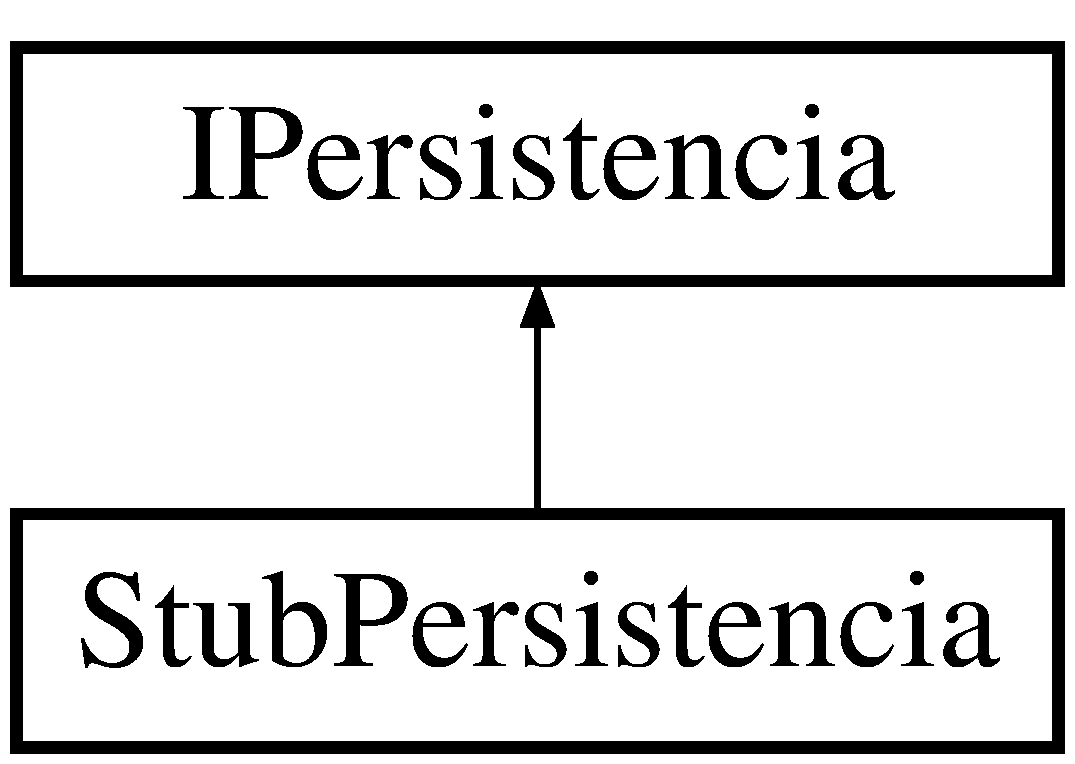
\includegraphics[height=2.000000cm]{class_i_persistencia}
\end{center}
\end{figure}
\subsection*{Public Member Functions}
\begin{DoxyCompactItemize}
\item 
\hypertarget{class_i_persistencia_aa821809bdcbc98729df56031ad7615db}{}\label{class_i_persistencia_aa821809bdcbc98729df56031ad7615db} 
virtual void {\bfseries executar} (const \hyperlink{class_comando_banco_dados}{Comando\+Banco\+Dados} $\ast$)=0  throw (runtime\+\_\+error)
\end{DoxyCompactItemize}


\subsection{Detailed Description}
Classe que contém os principais métodos dos comandos de persistencia da interface de negocio. 

Contém os protótipos dos métodos utilizados que se comunicam com a interface de negocio. 

The documentation for this class was generated from the following file\+:\begin{DoxyCompactItemize}
\item 
\hyperlink{_interfaces_8h}{Interfaces.\+h}\end{DoxyCompactItemize}

\hypertarget{class_i_u_autenticacao}{}\section{I\+U\+Autenticacao Class Reference}
\label{class_i_u_autenticacao}\index{I\+U\+Autenticacao@{I\+U\+Autenticacao}}


Classe que contém os principais métodos dos comandos da autenticação da interface.  




{\ttfamily \#include $<$Interfaces.\+h$>$}

Inheritance diagram for I\+U\+Autenticacao\+:\begin{figure}[H]
\begin{center}
\leavevmode
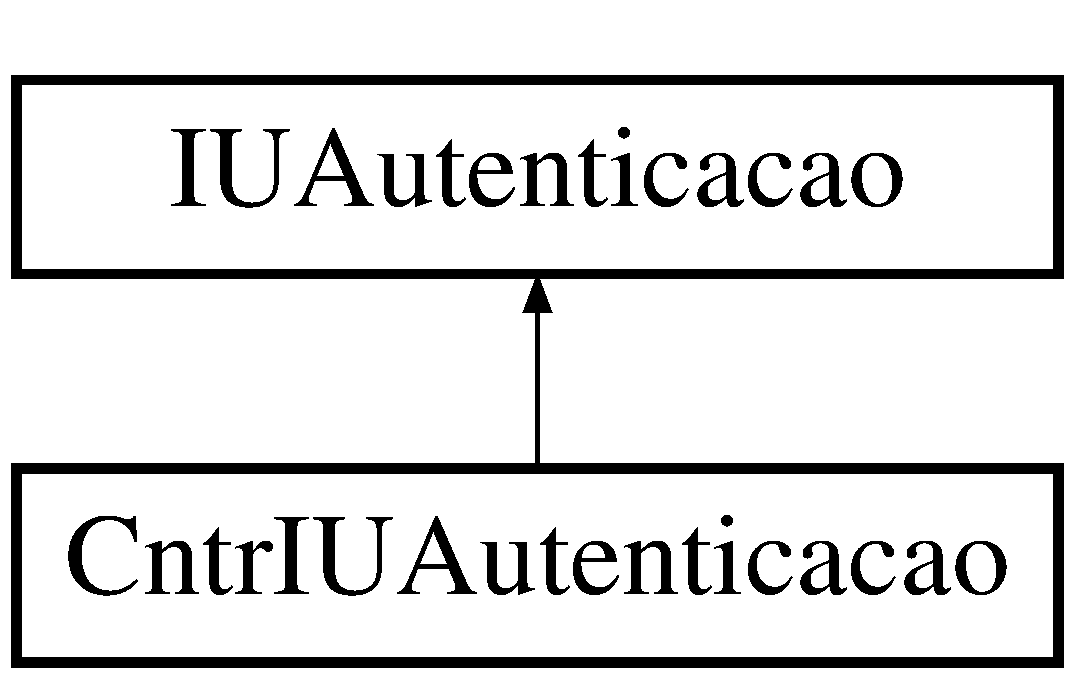
\includegraphics[height=2.000000cm]{class_i_u_autenticacao}
\end{center}
\end{figure}
\subsection*{Public Member Functions}
\begin{DoxyCompactItemize}
\item 
\hypertarget{class_i_u_autenticacao_ac963b141bda437bfd3ac425e9e6b9898}{}\label{class_i_u_autenticacao_ac963b141bda437bfd3ac425e9e6b9898} 
virtual \hyperlink{class_resultado_autenticacao}{Resultado\+Autenticacao} {\bfseries autenticar} ()=0  throw (runtime\+\_\+error)
\item 
\hypertarget{class_i_u_autenticacao_afaa4e4980ee10e2faaecb9ccfe524c61}{}\label{class_i_u_autenticacao_afaa4e4980ee10e2faaecb9ccfe524c61} 
virtual void {\bfseries set\+Cntr\+L\+N\+Autenticacao} (\hyperlink{class_i_l_n_autenticacao}{I\+L\+N\+Autenticacao} $\ast$)=0
\end{DoxyCompactItemize}


\subsection{Detailed Description}
Classe que contém os principais métodos dos comandos da autenticação da interface. 

Contém os protótipos dos métodos utilizados nas outras classes em \hyperlink{_controladoras_8h}{Controladoras.\+h} que se comunicam com a interface. 

The documentation for this class was generated from the following file\+:\begin{DoxyCompactItemize}
\item 
\hyperlink{_interfaces_8h}{Interfaces.\+h}\end{DoxyCompactItemize}

\hypertarget{class_i_u_desenvolvedor}{}\section{I\+U\+Desenvolvedor Class Reference}
\label{class_i_u_desenvolvedor}\index{I\+U\+Desenvolvedor@{I\+U\+Desenvolvedor}}


Classe que contém os principais métodos dos comandos do desenvolvedor da interface.  




{\ttfamily \#include $<$Interfaces.\+h$>$}

Inheritance diagram for I\+U\+Desenvolvedor\+:\begin{figure}[H]
\begin{center}
\leavevmode
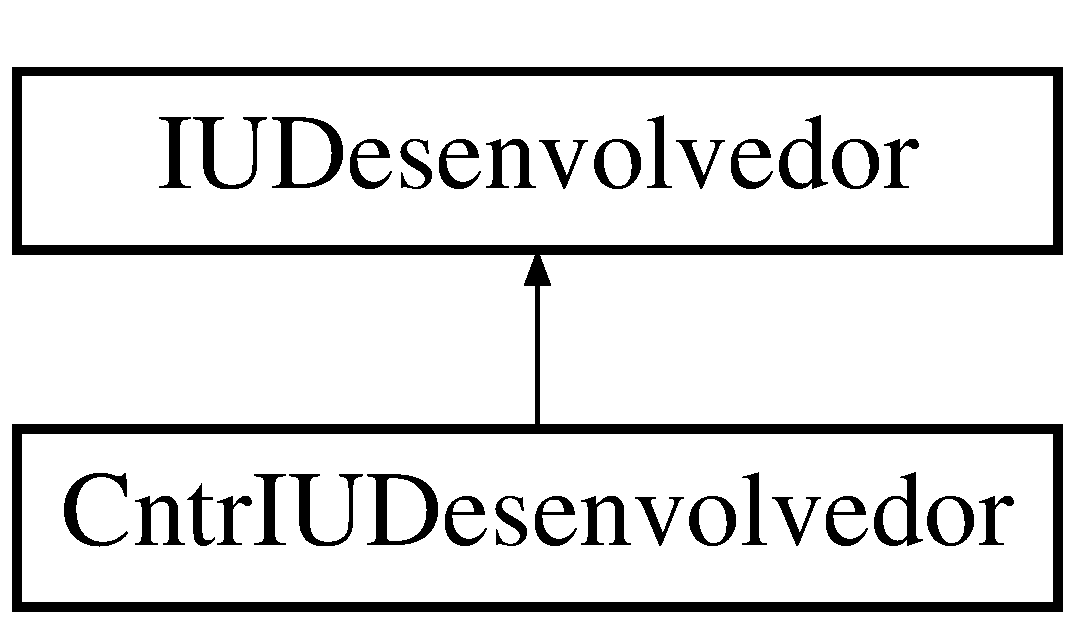
\includegraphics[height=2.000000cm]{class_i_u_desenvolvedor}
\end{center}
\end{figure}
\subsection*{Public Member Functions}
\begin{DoxyCompactItemize}
\item 
\hypertarget{class_i_u_desenvolvedor_a29c83b313e9ce403307ba7a5d54ce4a4}{}\label{class_i_u_desenvolvedor_a29c83b313e9ce403307ba7a5d54ce4a4} 
virtual void {\bfseries executar} (const \hyperlink{class_matricula}{Matricula} \&)=0  throw (runtime\+\_\+error)
\item 
\hypertarget{class_i_u_desenvolvedor_ad7e6fc192a682a9b4d3dd07866d9cc05}{}\label{class_i_u_desenvolvedor_ad7e6fc192a682a9b4d3dd07866d9cc05} 
virtual void {\bfseries set\+Cntr\+L\+N\+Desenvolvedor} (\hyperlink{class_i_l_n_desenvolvedor}{I\+L\+N\+Desenvolvedor} $\ast$)=0
\end{DoxyCompactItemize}


\subsection{Detailed Description}
Classe que contém os principais métodos dos comandos do desenvolvedor da interface. 

Contém os protótipos dos métodos utilizados nas outras classes em \hyperlink{_controladoras_8h}{Controladoras.\+h} que se comunicam com a interface. 

The documentation for this class was generated from the following file\+:\begin{DoxyCompactItemize}
\item 
\hyperlink{_interfaces_8h}{Interfaces.\+h}\end{DoxyCompactItemize}

\hypertarget{class_i_u_gerente_projeto}{}\section{I\+U\+Gerente\+Projeto Class Reference}
\label{class_i_u_gerente_projeto}\index{I\+U\+Gerente\+Projeto@{I\+U\+Gerente\+Projeto}}


Classe que contém os principais métodos dos comandos do gerente de projeto da interface.  




{\ttfamily \#include $<$Interfaces.\+h$>$}

Inheritance diagram for I\+U\+Gerente\+Projeto\+:\begin{figure}[H]
\begin{center}
\leavevmode
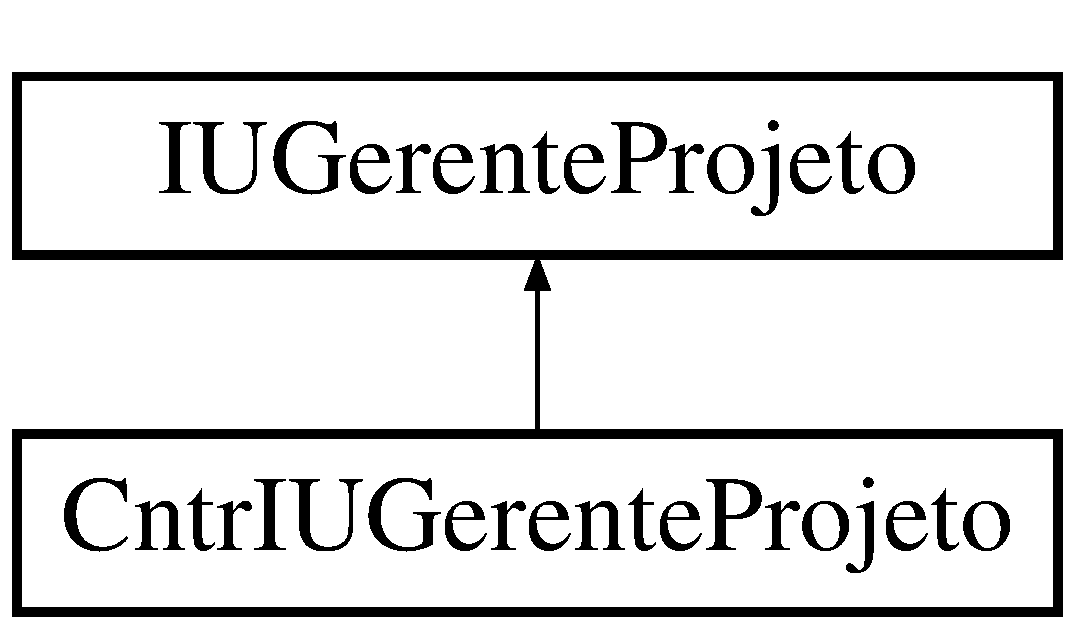
\includegraphics[height=2.000000cm]{class_i_u_gerente_projeto}
\end{center}
\end{figure}
\subsection*{Public Member Functions}
\begin{DoxyCompactItemize}
\item 
\hypertarget{class_i_u_gerente_projeto_a71b17efb4677cb13424e062948161626}{}\label{class_i_u_gerente_projeto_a71b17efb4677cb13424e062948161626} 
virtual void {\bfseries executar} (const \hyperlink{class_matricula}{Matricula} \&)=0  throw (runtime\+\_\+error)
\item 
\hypertarget{class_i_u_gerente_projeto_a056626862d1de6b472a163dc9350004e}{}\label{class_i_u_gerente_projeto_a056626862d1de6b472a163dc9350004e} 
virtual void {\bfseries set\+Cntr\+L\+N\+Gerente\+Projeto} (\hyperlink{class_i_l_n_gerente_projeto}{I\+L\+N\+Gerente\+Projeto} $\ast$)=0
\end{DoxyCompactItemize}


\subsection{Detailed Description}
Classe que contém os principais métodos dos comandos do gerente de projeto da interface. 

Contém os protótipos dos métodos utilizados nas outras classes em \hyperlink{_controladoras_8h}{Controladoras.\+h} que se comunicam com a interface. 

The documentation for this class was generated from the following file\+:\begin{DoxyCompactItemize}
\item 
\hyperlink{_interfaces_8h}{Interfaces.\+h}\end{DoxyCompactItemize}

\hypertarget{class_i_u_gerente_sistema}{}\section{I\+U\+Gerente\+Sistema Class Reference}
\label{class_i_u_gerente_sistema}\index{I\+U\+Gerente\+Sistema@{I\+U\+Gerente\+Sistema}}


Classe que contém os principais métodos dos comandos do gerente de sistema da interface.  




{\ttfamily \#include $<$Interfaces.\+h$>$}

Inheritance diagram for I\+U\+Gerente\+Sistema\+:\begin{figure}[H]
\begin{center}
\leavevmode
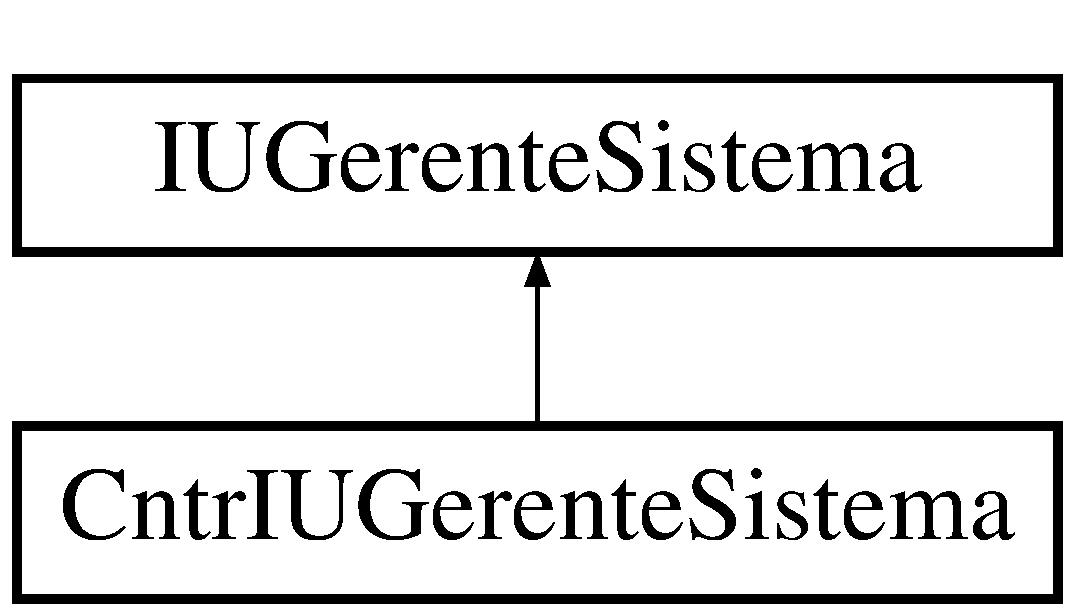
\includegraphics[height=2.000000cm]{class_i_u_gerente_sistema}
\end{center}
\end{figure}
\subsection*{Public Member Functions}
\begin{DoxyCompactItemize}
\item 
\hypertarget{class_i_u_gerente_sistema_ae9f231069ed7ff34998605a4c4396e37}{}\label{class_i_u_gerente_sistema_ae9f231069ed7ff34998605a4c4396e37} 
virtual void {\bfseries executar} (const \hyperlink{class_matricula}{Matricula} \&)=0  throw (runtime\+\_\+error)
\item 
\hypertarget{class_i_u_gerente_sistema_afe66d7bf2068a5f06e58310802479507}{}\label{class_i_u_gerente_sistema_afe66d7bf2068a5f06e58310802479507} 
virtual void {\bfseries set\+Cntr\+L\+N\+Gerente\+Sistema} (\hyperlink{class_i_l_n_gerente_sistema}{I\+L\+N\+Gerente\+Sistema} $\ast$)=0
\end{DoxyCompactItemize}


\subsection{Detailed Description}
Classe que contém os principais métodos dos comandos do gerente de sistema da interface. 

Contém os protótipos dos métodos utilizados nas outras classes em \hyperlink{_controladoras_8h}{Controladoras.\+h} que se comunicam com a interface. 

The documentation for this class was generated from the following file\+:\begin{DoxyCompactItemize}
\item 
\hyperlink{_interfaces_8h}{Interfaces.\+h}\end{DoxyCompactItemize}

\hypertarget{class_i_u_projeto}{}\section{I\+U\+Projeto Class Reference}
\label{class_i_u_projeto}\index{I\+U\+Projeto@{I\+U\+Projeto}}


Classe que contém os principais métodos dos comandos do projeto da interface.  




{\ttfamily \#include $<$Interfaces.\+h$>$}

Inheritance diagram for I\+U\+Projeto\+:\begin{figure}[H]
\begin{center}
\leavevmode
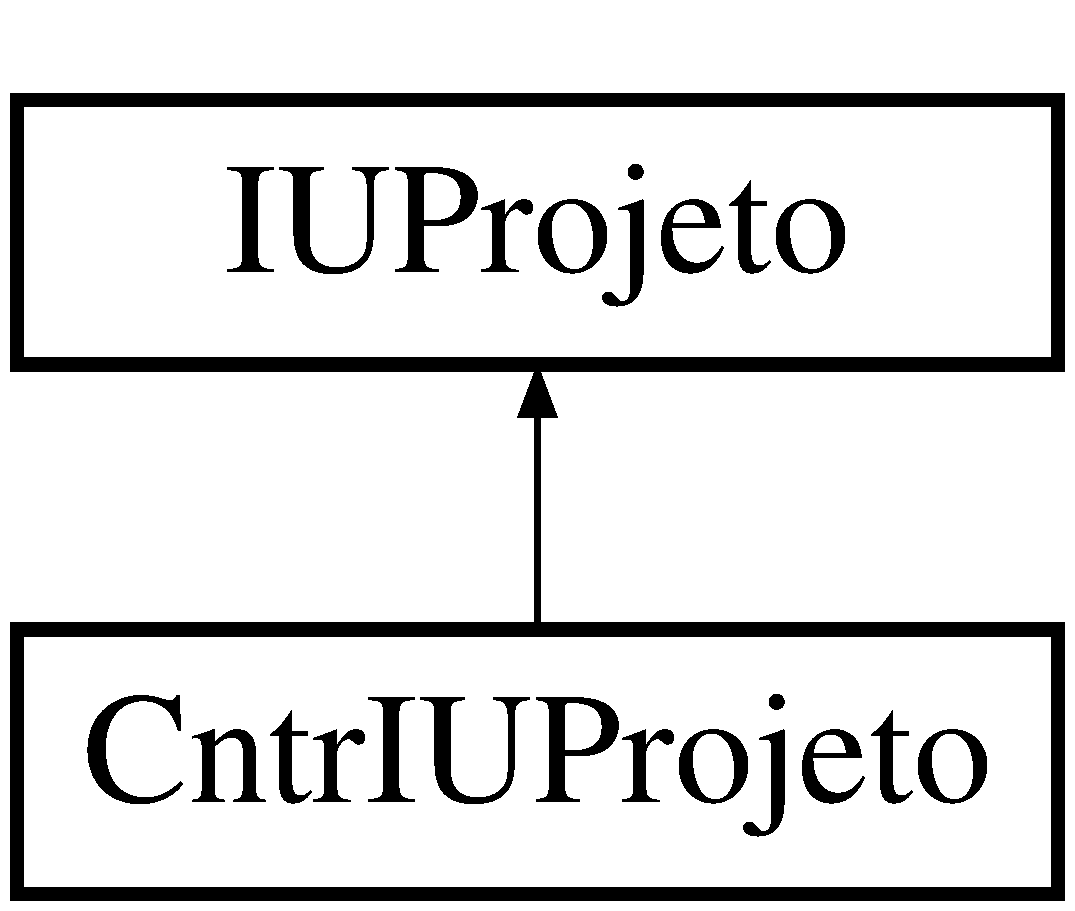
\includegraphics[height=2.000000cm]{class_i_u_projeto}
\end{center}
\end{figure}
\subsection*{Public Member Functions}
\begin{DoxyCompactItemize}
\item 
\hypertarget{class_i_u_projeto_ae5e911cacd0c88f2306df132c70027a5}{}\label{class_i_u_projeto_ae5e911cacd0c88f2306df132c70027a5} 
virtual void {\bfseries executar} (const \hyperlink{class_matricula}{Matricula} \&)=0  throw (runtime\+\_\+error)
\item 
\hypertarget{class_i_u_projeto_ac5a532baf383314cb2e4836aa69a7447}{}\label{class_i_u_projeto_ac5a532baf383314cb2e4836aa69a7447} 
virtual void {\bfseries set\+Cntr\+L\+N\+Projeto} (\hyperlink{class_i_l_n_projeto}{I\+L\+N\+Projeto} $\ast$)=0
\end{DoxyCompactItemize}


\subsection{Detailed Description}
Classe que contém os principais métodos dos comandos do projeto da interface. 

Contém os protótipos dos métodos utilizados nas outras classes em \hyperlink{_controladoras_8h}{Controladoras.\+h} que se comunicam com a interface. 

The documentation for this class was generated from the following file\+:\begin{DoxyCompactItemize}
\item 
\hyperlink{_interfaces_8h}{Interfaces.\+h}\end{DoxyCompactItemize}

\hypertarget{class_matricula}{}\section{Matricula Class Reference}
\label{class_matricula}\index{Matricula@{Matricula}}


Classe que cont�m os principais m�todos da matricula do dominio.  




{\ttfamily \#include $<$Dominio.\+h$>$}

\subsection*{Public Member Functions}
\begin{DoxyCompactItemize}
\item 
\hypertarget{class_matricula_ad0e207a892bf8ae631a9374d9998996c}{}\label{class_matricula_ad0e207a892bf8ae631a9374d9998996c} 
{\bfseries Matricula} (string)
\item 
\hypertarget{class_matricula_af5fa061fc9bc4adeee8c0d607de9aa87}{}\label{class_matricula_af5fa061fc9bc4adeee8c0d607de9aa87} 
void {\bfseries set\+Matricula} (string)  throw (invalid\+\_\+argument)
\item 
\hypertarget{class_matricula_aae1b9dfd6eec08ad9aa69b209fbc72d7}{}\label{class_matricula_aae1b9dfd6eec08ad9aa69b209fbc72d7} 
string {\bfseries get\+Matricula} () const
\item 
\hypertarget{class_matricula_a8e123daaaf6908f768ac88ac58664658}{}\label{class_matricula_a8e123daaaf6908f768ac88ac58664658} 
void {\bfseries is\+Matricula\+Valid} (string)  throw (invalid\+\_\+argument)
\end{DoxyCompactItemize}


\subsection{Detailed Description}
Classe que cont�m os principais m�todos da matricula do dominio. 

Cont�m os prot�tipos dos m�todos do nome referente ao dom�nio do sistema. 

The documentation for this class was generated from the following file\+:\begin{DoxyCompactItemize}
\item 
\hyperlink{_dominio_8h}{Dominio.\+h}\end{DoxyCompactItemize}

\hypertarget{class_nome}{}\section{Nome Class Reference}
\label{class_nome}\index{Nome@{Nome}}


Classe que cont�m os principais m�todos do nome do dominio.  




{\ttfamily \#include $<$Dominio.\+h$>$}

\subsection*{Public Member Functions}
\begin{DoxyCompactItemize}
\item 
\hypertarget{class_nome_a5a31c8dec7272e90a3d5cb59cece8c28}{}\label{class_nome_a5a31c8dec7272e90a3d5cb59cece8c28} 
{\bfseries Nome} (string)
\item 
\hypertarget{class_nome_ab1507b81047efb89b50b6be0d33c08e5}{}\label{class_nome_ab1507b81047efb89b50b6be0d33c08e5} 
void {\bfseries set\+Nome} (string)  throw (invalid\+\_\+argument)
\item 
\hypertarget{class_nome_a1c08f5b9827a1e97a2631196ff99fdef}{}\label{class_nome_a1c08f5b9827a1e97a2631196ff99fdef} 
string {\bfseries get\+Nome} () const
\item 
\hypertarget{class_nome_a5553f450b406d1660ccae3d356dd481c}{}\label{class_nome_a5553f450b406d1660ccae3d356dd481c} 
void {\bfseries is\+Nome\+Valid} (string)  throw (invalid\+\_\+argument)
\end{DoxyCompactItemize}


\subsection{Detailed Description}
Classe que cont�m os principais m�todos do nome do dominio. 

Cont�m os prot�tipos dos m�todos do nome referente ao dom�nio do sistema. 

The documentation for this class was generated from the following file\+:\begin{DoxyCompactItemize}
\item 
\hyperlink{_dominio_8h}{Dominio.\+h}\end{DoxyCompactItemize}

\hypertarget{class_projeto}{}\section{Projeto Class Reference}
\label{class_projeto}\index{Projeto@{Projeto}}


Classe que cont�m os principais m�todos da entidade de projeto.  




{\ttfamily \#include $<$Entidade.\+h$>$}

\subsection*{Public Attributes}
\begin{DoxyCompactItemize}
\item 
\hypertarget{class_projeto_ad924e0c60bd0ca40b00cf51b4c08dac2}{}\label{class_projeto_ad924e0c60bd0ca40b00cf51b4c08dac2} 
\hyperlink{class_nome}{Nome} {\bfseries nome}
\item 
\hypertarget{class_projeto_a123003d8c4d9eb4dcb27168cb9a10c45}{}\label{class_projeto_a123003d8c4d9eb4dcb27168cb9a10c45} 
\hyperlink{class_codigo_projeto}{Codigo\+Projeto} {\bfseries codigo\+Projeto}
\item 
\hypertarget{class_projeto_a58e9b71bcb6cf0c00061e962e8e390cd}{}\label{class_projeto_a58e9b71bcb6cf0c00061e962e8e390cd} 
\hyperlink{class_gerente_projeto}{Gerente\+Projeto} {\bfseries gerente\+Projeto}
\item 
\hypertarget{class_projeto_a63341acf1663e7bd94cc72105d4499f1}{}\label{class_projeto_a63341acf1663e7bd94cc72105d4499f1} 
\hyperlink{class_data}{Data} {\bfseries data\+Inicio}
\item 
\hypertarget{class_projeto_aac85cd2e118ed6ecc76ab4535e57a4c0}{}\label{class_projeto_aac85cd2e118ed6ecc76ab4535e57a4c0} 
\hyperlink{class_data}{Data} {\bfseries data\+Fim}
\item 
\hypertarget{class_projeto_aa3c4472af5a4b82b35ba042eecf90fe5}{}\label{class_projeto_aa3c4472af5a4b82b35ba042eecf90fe5} 
\hyperlink{class_custo}{Custo} {\bfseries custo\+Atual}
\item 
\hypertarget{class_projeto_ad4f079289614c728f77116cd1267669e}{}\label{class_projeto_ad4f079289614c728f77116cd1267669e} 
\hyperlink{class_custo}{Custo} {\bfseries custo\+Previsto}
\item 
\hypertarget{class_projeto_a4ec5c9cad7f3e782e7a4928ed3282cea}{}\label{class_projeto_a4ec5c9cad7f3e782e7a4928ed3282cea} 
\hyperlink{class_estado_projeto}{Estado\+Projeto} {\bfseries estado\+Projeto}
\item 
\hypertarget{class_projeto_a50f13adb6fcce8d09fc7ae1d175c9bd5}{}\label{class_projeto_a50f13adb6fcce8d09fc7ae1d175c9bd5} 
\hyperlink{class_fase_projeto}{Fase\+Projeto} {\bfseries fase\+Projeto}
\end{DoxyCompactItemize}


\subsection{Detailed Description}
Classe que cont�m os principais m�todos da entidade de projeto. 

Cont�m os prot�tipos dos m�todos da classe projeto referente �s entidades do sistema. 

The documentation for this class was generated from the following file\+:\begin{DoxyCompactItemize}
\item 
\hyperlink{_entidade_8h}{Entidade.\+h}\end{DoxyCompactItemize}

\hypertarget{class_resultado}{}\section{Resultado Class Reference}
\label{class_resultado}\index{Resultado@{Resultado}}


Classe que cont�m os principais m�todos da entidade de \hyperlink{class_resultado}{Resultado}.  




{\ttfamily \#include $<$Entidade.\+h$>$}

Inheritance diagram for Resultado\+:\begin{figure}[H]
\begin{center}
\leavevmode
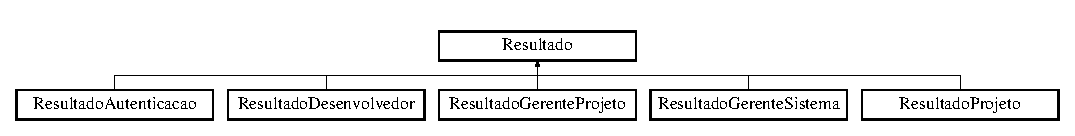
\includegraphics[height=1.374233cm]{class_resultado}
\end{center}
\end{figure}
\subsection*{Public Member Functions}
\begin{DoxyCompactItemize}
\item 
\hypertarget{class_resultado_ab0c3c0ed280eefb95e89d90dc7e239e2}{}\label{class_resultado_ab0c3c0ed280eefb95e89d90dc7e239e2} 
void {\bfseries set\+Valor} (int valor)
\item 
\hypertarget{class_resultado_a029dc1436d6ed7963b5b90400e972e15}{}\label{class_resultado_a029dc1436d6ed7963b5b90400e972e15} 
int {\bfseries get\+Valor} () const
\end{DoxyCompactItemize}
\subsection*{Static Public Attributes}
\begin{DoxyCompactItemize}
\item 
\hypertarget{class_resultado_a234e15461a4fcccbbb82852278cd092f}{}\label{class_resultado_a234e15461a4fcccbbb82852278cd092f} 
static const int {\bfseries S\+U\+C\+E\+S\+SO} = 0
\item 
\hypertarget{class_resultado_a9a1c136d1a2189c25e6eaff45182083b}{}\label{class_resultado_a9a1c136d1a2189c25e6eaff45182083b} 
static const int {\bfseries F\+A\+L\+HA} = 1
\end{DoxyCompactItemize}
\subsection*{Protected Attributes}
\begin{DoxyCompactItemize}
\item 
\hypertarget{class_resultado_a452e65ac80b05f5081642c869d960ac9}{}\label{class_resultado_a452e65ac80b05f5081642c869d960ac9} 
int {\bfseries valor}
\end{DoxyCompactItemize}


\subsection{Detailed Description}
Classe que cont�m os principais m�todos da entidade de \hyperlink{class_resultado}{Resultado}. 

Cont�m os prot�tipos dos m�todos da classe resultado referente �s entidades do sistema. 

The documentation for this class was generated from the following file\+:\begin{DoxyCompactItemize}
\item 
\hyperlink{_entidade_8h}{Entidade.\+h}\end{DoxyCompactItemize}

\hypertarget{class_resultado_autenticacao}{}\section{Resultado\+Autenticacao Class Reference}
\label{class_resultado_autenticacao}\index{Resultado\+Autenticacao@{Resultado\+Autenticacao}}


Classe que cont�m os principais m�todos da entidade de \hyperlink{class_resultado}{Resultado} de autenticacao.  




{\ttfamily \#include $<$Entidade.\+h$>$}

Inheritance diagram for Resultado\+Autenticacao\+:\begin{figure}[H]
\begin{center}
\leavevmode
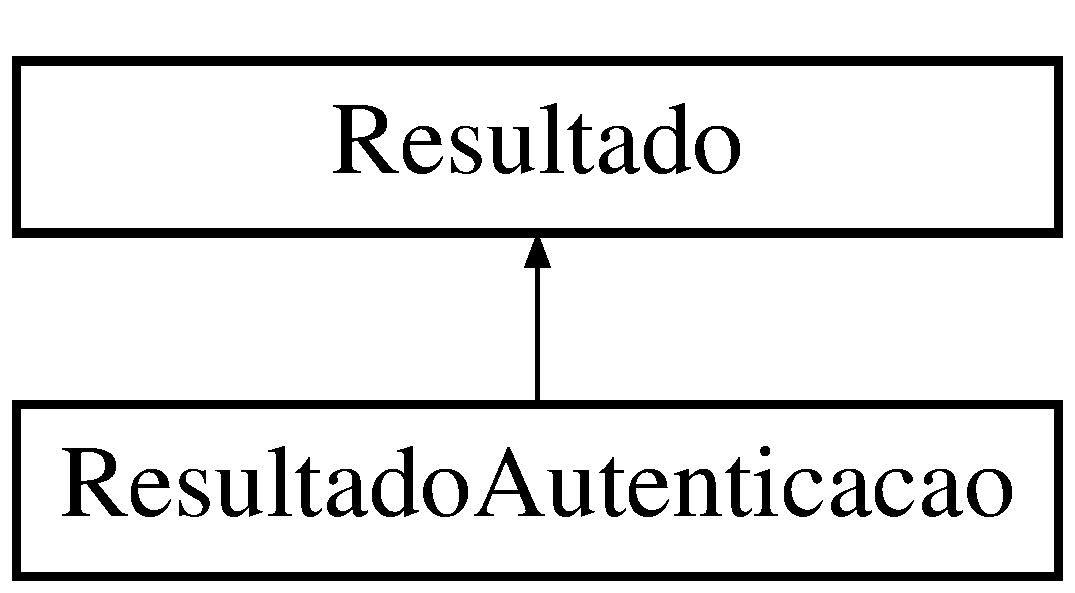
\includegraphics[height=2.000000cm]{class_resultado_autenticacao}
\end{center}
\end{figure}
\subsection*{Public Member Functions}
\begin{DoxyCompactItemize}
\item 
\hypertarget{class_resultado_autenticacao_a69f466e5f80b2b70ced9e387d2b7ebc5}{}\label{class_resultado_autenticacao_a69f466e5f80b2b70ced9e387d2b7ebc5} 
void {\bfseries set\+Matricula} (const \hyperlink{class_matricula}{Matricula} \&matricula)
\item 
\hypertarget{class_resultado_autenticacao_a64ae9715511693ba82a94ea178593552}{}\label{class_resultado_autenticacao_a64ae9715511693ba82a94ea178593552} 
\hyperlink{class_matricula}{Matricula} {\bfseries get\+Matricula} () const
\end{DoxyCompactItemize}
\subsection*{Additional Inherited Members}


\subsection{Detailed Description}
Classe que cont�m os principais m�todos da entidade de \hyperlink{class_resultado}{Resultado} de autenticacao. 

Cont�m os prot�tipos dos m�todos da classe \hyperlink{class_resultado_autenticacao}{Resultado\+Autenticacao} referente �s entidades do sistema. 

The documentation for this class was generated from the following file\+:\begin{DoxyCompactItemize}
\item 
\hyperlink{_entidade_8h}{Entidade.\+h}\end{DoxyCompactItemize}

\hypertarget{class_resultado_desenvolvedor}{}\section{Resultado\+Desenvolvedor Class Reference}
\label{class_resultado_desenvolvedor}\index{Resultado\+Desenvolvedor@{Resultado\+Desenvolvedor}}


Classe que cont�m os principais m�todos da entidade de \hyperlink{class_resultado}{Resultado} de desenvolvedor.  




{\ttfamily \#include $<$Entidade.\+h$>$}

Inheritance diagram for Resultado\+Desenvolvedor\+:\begin{figure}[H]
\begin{center}
\leavevmode
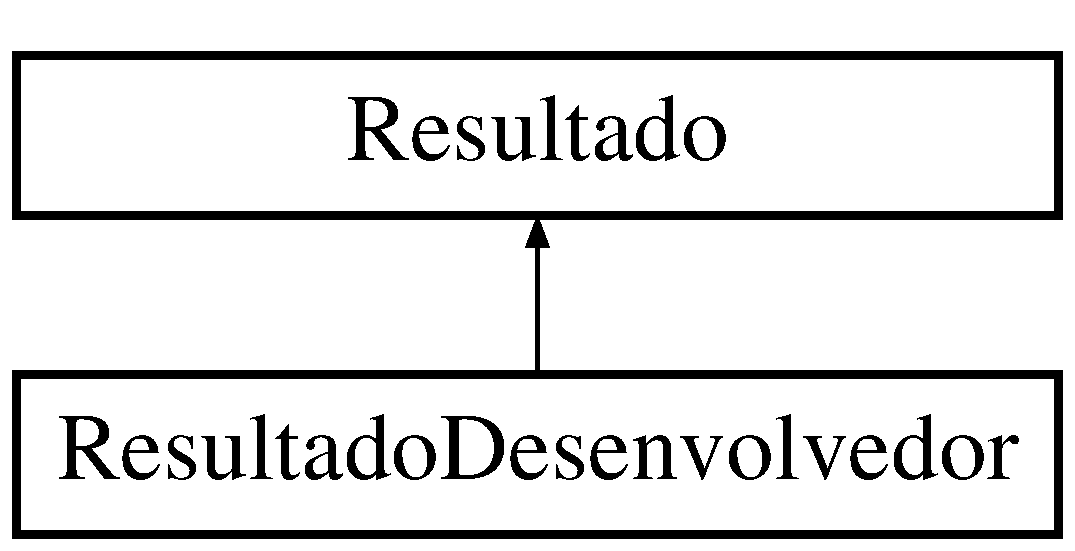
\includegraphics[height=2.000000cm]{class_resultado_desenvolvedor}
\end{center}
\end{figure}
\subsection*{Public Member Functions}
\begin{DoxyCompactItemize}
\item 
\hypertarget{class_resultado_desenvolvedor_abb13ccef2fb1a96aed08ac9026f0d42f}{}\label{class_resultado_desenvolvedor_abb13ccef2fb1a96aed08ac9026f0d42f} 
void {\bfseries set\+Desenvolvedor} (const \hyperlink{class_desenvolvedor}{Desenvolvedor} \&desenvolvedor)
\item 
\hypertarget{class_resultado_desenvolvedor_a4cf4381ad5927ed46ad631fc15c11759}{}\label{class_resultado_desenvolvedor_a4cf4381ad5927ed46ad631fc15c11759} 
\hyperlink{class_desenvolvedor}{Desenvolvedor} {\bfseries get\+Desenvolvedor} () const
\end{DoxyCompactItemize}
\subsection*{Additional Inherited Members}


\subsection{Detailed Description}
Classe que cont�m os principais m�todos da entidade de \hyperlink{class_resultado}{Resultado} de desenvolvedor. 

Cont�m os prot�tipos dos m�todos da classe resultado de desenvolvedor referente �s entidades do sistema. 

The documentation for this class was generated from the following file\+:\begin{DoxyCompactItemize}
\item 
\hyperlink{_entidade_8h}{Entidade.\+h}\end{DoxyCompactItemize}

\hypertarget{class_resultado_gerente_projeto}{}\section{Resultado\+Gerente\+Projeto Class Reference}
\label{class_resultado_gerente_projeto}\index{Resultado\+Gerente\+Projeto@{Resultado\+Gerente\+Projeto}}


Classe que cont�m os principais m�todos da entidade de \hyperlink{class_resultado}{Resultado} de Gerente de \hyperlink{class_projeto}{Projeto}.  




{\ttfamily \#include $<$Entidade.\+h$>$}

Inheritance diagram for Resultado\+Gerente\+Projeto\+:\begin{figure}[H]
\begin{center}
\leavevmode
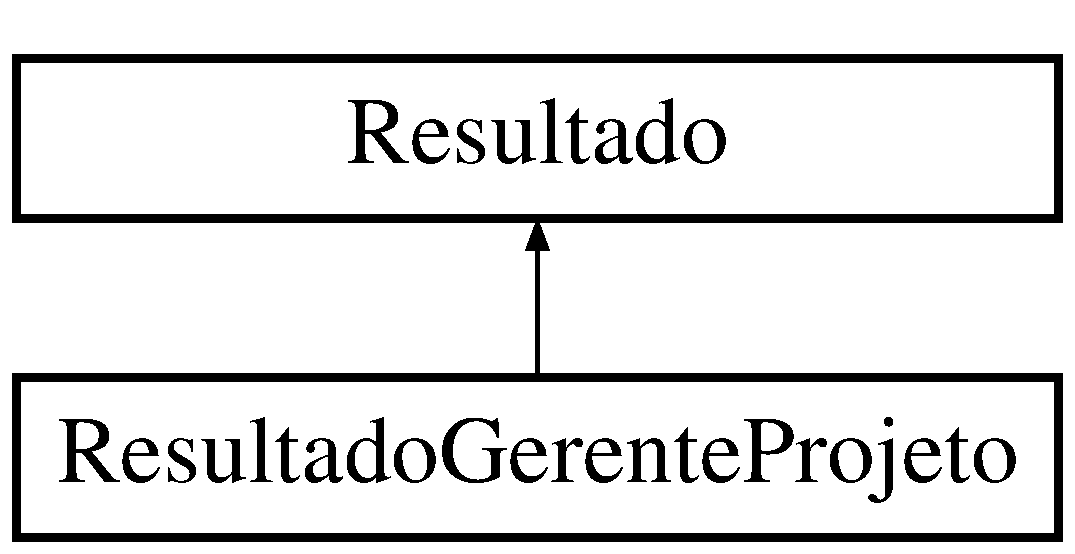
\includegraphics[height=2.000000cm]{class_resultado_gerente_projeto}
\end{center}
\end{figure}
\subsection*{Public Member Functions}
\begin{DoxyCompactItemize}
\item 
\hypertarget{class_resultado_gerente_projeto_ac7c1e1b88b10ce401bc7164551b9e3c0}{}\label{class_resultado_gerente_projeto_ac7c1e1b88b10ce401bc7164551b9e3c0} 
void {\bfseries set\+Gerente\+Projeto} (const \hyperlink{class_gerente_projeto}{Gerente\+Projeto} \&gerente\+Projeto)
\item 
\hypertarget{class_resultado_gerente_projeto_ae54cb1c26dd5125f1717b0199953395b}{}\label{class_resultado_gerente_projeto_ae54cb1c26dd5125f1717b0199953395b} 
\hyperlink{class_gerente_projeto}{Gerente\+Projeto} {\bfseries get\+Gerente\+Projeto} () const
\end{DoxyCompactItemize}
\subsection*{Additional Inherited Members}


\subsection{Detailed Description}
Classe que cont�m os principais m�todos da entidade de \hyperlink{class_resultado}{Resultado} de Gerente de \hyperlink{class_projeto}{Projeto}. 

Cont�m os prot�tipos dos m�todos da classe \hyperlink{class_resultado}{Resultado} de gerente de projeto referente �s entidades do sistema. 

The documentation for this class was generated from the following file\+:\begin{DoxyCompactItemize}
\item 
\hyperlink{_entidade_8h}{Entidade.\+h}\end{DoxyCompactItemize}

\hypertarget{class_resultado_gerente_sistema}{}\section{Resultado\+Gerente\+Sistema Class Reference}
\label{class_resultado_gerente_sistema}\index{Resultado\+Gerente\+Sistema@{Resultado\+Gerente\+Sistema}}


Classe que cont�m os principais m�todos da entidade de resultado de gerente de sistema.  




{\ttfamily \#include $<$Entidade.\+h$>$}

Inheritance diagram for Resultado\+Gerente\+Sistema\+:\begin{figure}[H]
\begin{center}
\leavevmode
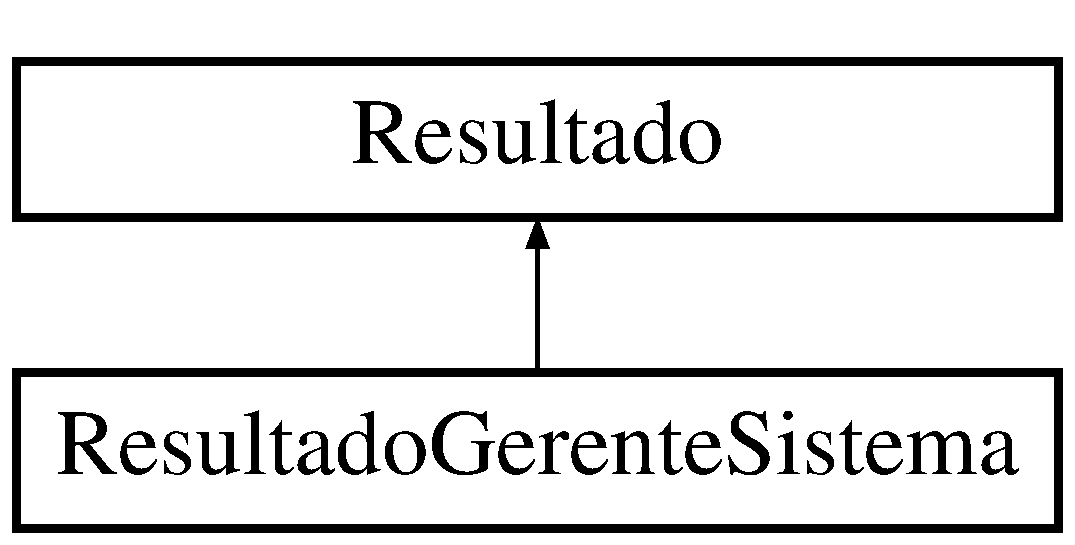
\includegraphics[height=2.000000cm]{class_resultado_gerente_sistema}
\end{center}
\end{figure}
\subsection*{Public Member Functions}
\begin{DoxyCompactItemize}
\item 
\hypertarget{class_resultado_gerente_sistema_a7c47e4e3573d4fcaaf1b47bd2043778b}{}\label{class_resultado_gerente_sistema_a7c47e4e3573d4fcaaf1b47bd2043778b} 
void {\bfseries set\+Gerente\+Sistema} (const \hyperlink{class_gerente_sistema}{Gerente\+Sistema} \&gerente\+Sistema)
\item 
\hypertarget{class_resultado_gerente_sistema_ad6426d05c4b2f51672ee9690c1702e10}{}\label{class_resultado_gerente_sistema_ad6426d05c4b2f51672ee9690c1702e10} 
\hyperlink{class_gerente_sistema}{Gerente\+Sistema} {\bfseries get\+Gerente\+Sistema} () const
\end{DoxyCompactItemize}
\subsection*{Additional Inherited Members}


\subsection{Detailed Description}
Classe que cont�m os principais m�todos da entidade de resultado de gerente de sistema. 

Cont�m os prot�tipos dos m�todos da classe resultado de gerente de sistema referente �s entidades do sistema. 

The documentation for this class was generated from the following file\+:\begin{DoxyCompactItemize}
\item 
\hyperlink{_entidade_8h}{Entidade.\+h}\end{DoxyCompactItemize}

\hypertarget{class_resultado_projeto}{}\section{Resultado\+Projeto Class Reference}
\label{class_resultado_projeto}\index{Resultado\+Projeto@{Resultado\+Projeto}}


Classe que cont�m os principais m�todos da entidade de \hyperlink{class_resultado}{Resultado} de projeto.  




{\ttfamily \#include $<$Entidade.\+h$>$}

Inheritance diagram for Resultado\+Projeto\+:\begin{figure}[H]
\begin{center}
\leavevmode
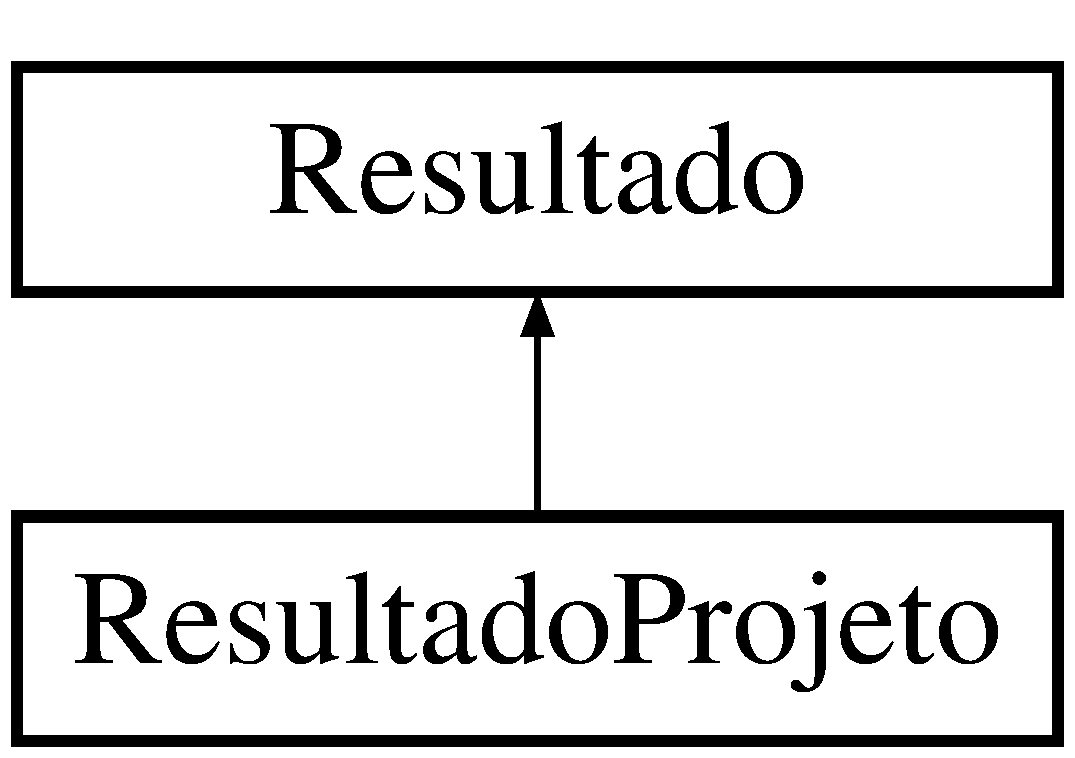
\includegraphics[height=2.000000cm]{class_resultado_projeto}
\end{center}
\end{figure}
\subsection*{Public Member Functions}
\begin{DoxyCompactItemize}
\item 
\hypertarget{class_resultado_projeto_a99711cf9a7e65da235a655c5a1d70e39}{}\label{class_resultado_projeto_a99711cf9a7e65da235a655c5a1d70e39} 
void {\bfseries set\+Projeto} (const \hyperlink{class_projeto}{Projeto} \&projeto)
\item 
\hypertarget{class_resultado_projeto_a7b8f2a0cb954e7d08b807e859d568cac}{}\label{class_resultado_projeto_a7b8f2a0cb954e7d08b807e859d568cac} 
\hyperlink{class_projeto}{Projeto} {\bfseries get\+Projeto} () const
\end{DoxyCompactItemize}
\subsection*{Additional Inherited Members}


\subsection{Detailed Description}
Classe que cont�m os principais m�todos da entidade de \hyperlink{class_resultado}{Resultado} de projeto. 

Cont�m os prot�tipos dos m�todos da classe resultado de projeto referente �s entidades do sistema. 

The documentation for this class was generated from the following file\+:\begin{DoxyCompactItemize}
\item 
\hyperlink{_entidade_8h}{Entidade.\+h}\end{DoxyCompactItemize}

\hypertarget{class_senha}{}\section{Senha Class Reference}
\label{class_senha}\index{Senha@{Senha}}


Classe que cont�m os principais m�todos da senha do dominio.  




{\ttfamily \#include $<$Dominio.\+h$>$}

\subsection*{Public Member Functions}
\begin{DoxyCompactItemize}
\item 
\hypertarget{class_senha_a9f4ad62d7b5add66ec2647eb3b2aef6f}{}\label{class_senha_a9f4ad62d7b5add66ec2647eb3b2aef6f} 
{\bfseries Senha} (string)
\item 
\hypertarget{class_senha_a735e4bf5f65cc8d28daa7dbf202fd999}{}\label{class_senha_a735e4bf5f65cc8d28daa7dbf202fd999} 
void {\bfseries set\+Senha} (string)  throw (invalid\+\_\+argument)
\item 
\hypertarget{class_senha_a1cc904431d0a8287d0b22dee3e9d34ae}{}\label{class_senha_a1cc904431d0a8287d0b22dee3e9d34ae} 
string {\bfseries get\+Senha} () const
\item 
\hypertarget{class_senha_a86b20e798b2f1b8e95db57cca41e13b0}{}\label{class_senha_a86b20e798b2f1b8e95db57cca41e13b0} 
void {\bfseries is\+Senha\+Valid} (string)  throw (invalid\+\_\+argument)
\end{DoxyCompactItemize}


\subsection{Detailed Description}
Classe que cont�m os principais m�todos da senha do dominio. 

Cont�m os prot�tipos dos m�todos do nome referente ao dom�nio do sistema. 

The documentation for this class was generated from the following file\+:\begin{DoxyCompactItemize}
\item 
\hyperlink{_dominio_8h}{Dominio.\+h}\end{DoxyCompactItemize}

\hypertarget{class_stub_l_n_a_gerente}{}\section{Stub\+L\+N\+A\+Gerente Class Reference}
\label{class_stub_l_n_a_gerente}\index{Stub\+L\+N\+A\+Gerente@{Stub\+L\+N\+A\+Gerente}}


Classe que cont�m os m�todos dos stubs de gerente de sistema.  




{\ttfamily \#include $<$Stubs.\+h$>$}



\subsection{Detailed Description}
Classe que cont�m os m�todos dos stubs de gerente de sistema. 

Classe que cont�m os m�todos dos stubs de desenvolvedor.

Cont�m os prot�tipos dos m�todos da classe de stub referente ao gerente de sistema da logica de negocio.

Cont�m os prot�tipos dos m�todos da classe de stub referente ao desenvolvedor da logica de negocio. 

The documentation for this class was generated from the following file\+:\begin{DoxyCompactItemize}
\item 
\hyperlink{_stubs_8h}{Stubs.\+h}\end{DoxyCompactItemize}

\hypertarget{class_stub_l_n_autenticacao}{}\section{Stub\+L\+N\+Autenticacao Class Reference}
\label{class_stub_l_n_autenticacao}\index{Stub\+L\+N\+Autenticacao@{Stub\+L\+N\+Autenticacao}}


Classe que cont�m os m�todos dos stubs de autenticao.  




{\ttfamily \#include $<$Stubs.\+h$>$}

Inheritance diagram for Stub\+L\+N\+Autenticacao\+:\begin{figure}[H]
\begin{center}
\leavevmode
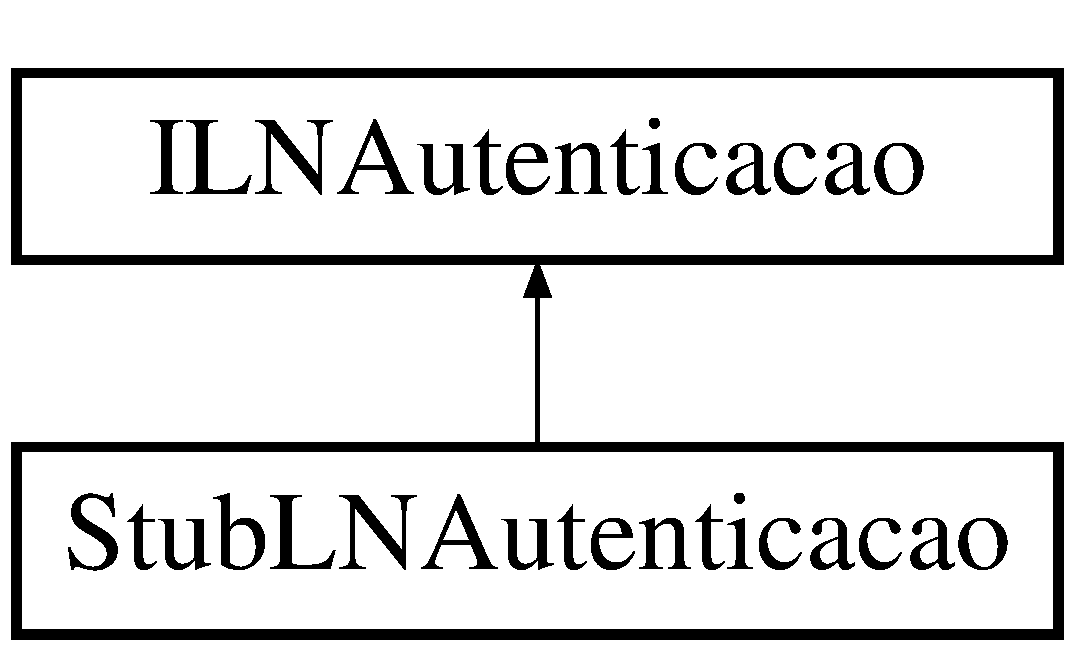
\includegraphics[height=2.000000cm]{class_stub_l_n_autenticacao}
\end{center}
\end{figure}
\subsection*{Public Member Functions}
\begin{DoxyCompactItemize}
\item 
\hypertarget{class_stub_l_n_autenticacao_a5b81ad78d0ff0e14c0d7c03022468742}{}\label{class_stub_l_n_autenticacao_a5b81ad78d0ff0e14c0d7c03022468742} 
\hyperlink{class_resultado_autenticacao}{Resultado\+Autenticacao} {\bfseries autenticar} (const \hyperlink{class_matricula}{Matricula} \&, const \hyperlink{class_senha}{Senha} \&)  throw (runtime\+\_\+error)
\end{DoxyCompactItemize}
\subsection*{Static Public Attributes}
\begin{DoxyCompactItemize}
\item 
\hypertarget{class_stub_l_n_autenticacao_aafd8b873e92597415b1b48436ba837e6}{}\label{class_stub_l_n_autenticacao_aafd8b873e92597415b1b48436ba837e6} 
static const string {\bfseries T\+R\+I\+G\+G\+E\+R\+\_\+\+F\+A\+L\+HA}
\item 
\hypertarget{class_stub_l_n_autenticacao_aae13659366a560e0c3903bb7bc29b5bc}{}\label{class_stub_l_n_autenticacao_aae13659366a560e0c3903bb7bc29b5bc} 
static const string {\bfseries T\+R\+I\+G\+G\+E\+R\+\_\+\+E\+R\+R\+O\+\_\+\+S\+I\+S\+T\+E\+MA}
\end{DoxyCompactItemize}


\subsection{Detailed Description}
Classe que cont�m os m�todos dos stubs de autenticao. 

Cont�m os prot�tipos dos m�todos da classe de stub referente a autenticacao da logica de negocio. 

The documentation for this class was generated from the following file\+:\begin{DoxyCompactItemize}
\item 
\hyperlink{_stubs_8h}{Stubs.\+h}\end{DoxyCompactItemize}

\hypertarget{class_stub_l_n_desenvolvedor}{}\section{Stub\+L\+N\+Desenvolvedor Class Reference}
\label{class_stub_l_n_desenvolvedor}\index{Stub\+L\+N\+Desenvolvedor@{Stub\+L\+N\+Desenvolvedor}}
Inheritance diagram for Stub\+L\+N\+Desenvolvedor\+:\begin{figure}[H]
\begin{center}
\leavevmode
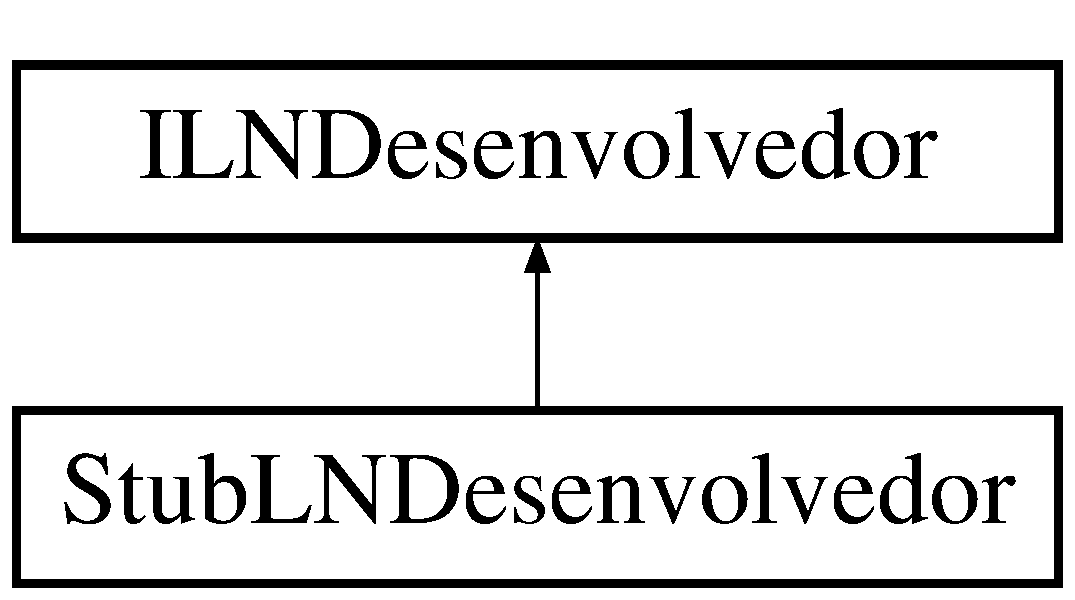
\includegraphics[height=2.000000cm]{class_stub_l_n_desenvolvedor}
\end{center}
\end{figure}
\subsection*{Public Member Functions}
\begin{DoxyCompactItemize}
\item 
\hypertarget{class_stub_l_n_desenvolvedor_a7b855ccbcd35bba830f66a6333d4df8d}{}\label{class_stub_l_n_desenvolvedor_a7b855ccbcd35bba830f66a6333d4df8d} 
\hyperlink{class_resultado_desenvolvedor}{Resultado\+Desenvolvedor} {\bfseries incluir} (const \hyperlink{class_desenvolvedor}{Desenvolvedor} \&)  throw (runtime\+\_\+error)
\item 
\hypertarget{class_stub_l_n_desenvolvedor_ad73c34044c2192cd68f9a44eb1e19ac0}{}\label{class_stub_l_n_desenvolvedor_ad73c34044c2192cd68f9a44eb1e19ac0} 
\hyperlink{class_resultado_desenvolvedor}{Resultado\+Desenvolvedor} {\bfseries remover} (const \hyperlink{class_matricula}{Matricula} \&)  throw (runtime\+\_\+error)
\item 
\hypertarget{class_stub_l_n_desenvolvedor_ad4334f0a1b64ba4e764f350c1ad3943b}{}\label{class_stub_l_n_desenvolvedor_ad4334f0a1b64ba4e764f350c1ad3943b} 
\hyperlink{class_resultado_desenvolvedor}{Resultado\+Desenvolvedor} {\bfseries pesquisar} (const \hyperlink{class_matricula}{Matricula} \&)  throw (runtime\+\_\+error)
\item 
\hypertarget{class_stub_l_n_desenvolvedor_aa023e2d85ea41e9e7d6056e93088998c}{}\label{class_stub_l_n_desenvolvedor_aa023e2d85ea41e9e7d6056e93088998c} 
\hyperlink{class_resultado_desenvolvedor}{Resultado\+Desenvolvedor} {\bfseries editar} (const \hyperlink{class_desenvolvedor}{Desenvolvedor} \&)  throw (runtime\+\_\+error)
\end{DoxyCompactItemize}


The documentation for this class was generated from the following file\+:\begin{DoxyCompactItemize}
\item 
\hyperlink{_stubs_8h}{Stubs.\+h}\end{DoxyCompactItemize}

\hypertarget{class_stub_l_n_gerente}{}\section{Stub\+L\+N\+Gerente Class Reference}
\label{class_stub_l_n_gerente}\index{Stub\+L\+N\+Gerente@{Stub\+L\+N\+Gerente}}


Classe que cont�m os m�todos dos stubs de Gerente de projeto.  




{\ttfamily \#include $<$Stubs.\+h$>$}



\subsection{Detailed Description}
Classe que cont�m os m�todos dos stubs de Gerente de projeto. 

Cont�m os prot�tipos dos m�todos da classe de stub referente ao gerente de projeto da logica de negocio. 

The documentation for this class was generated from the following file\+:\begin{DoxyCompactItemize}
\item 
\hyperlink{_stubs_8h}{Stubs.\+h}\end{DoxyCompactItemize}

\hypertarget{class_stub_l_n_gerente_projeto}{}\section{Stub\+L\+N\+Gerente\+Projeto Class Reference}
\label{class_stub_l_n_gerente_projeto}\index{Stub\+L\+N\+Gerente\+Projeto@{Stub\+L\+N\+Gerente\+Projeto}}
Inheritance diagram for Stub\+L\+N\+Gerente\+Projeto\+:\begin{figure}[H]
\begin{center}
\leavevmode
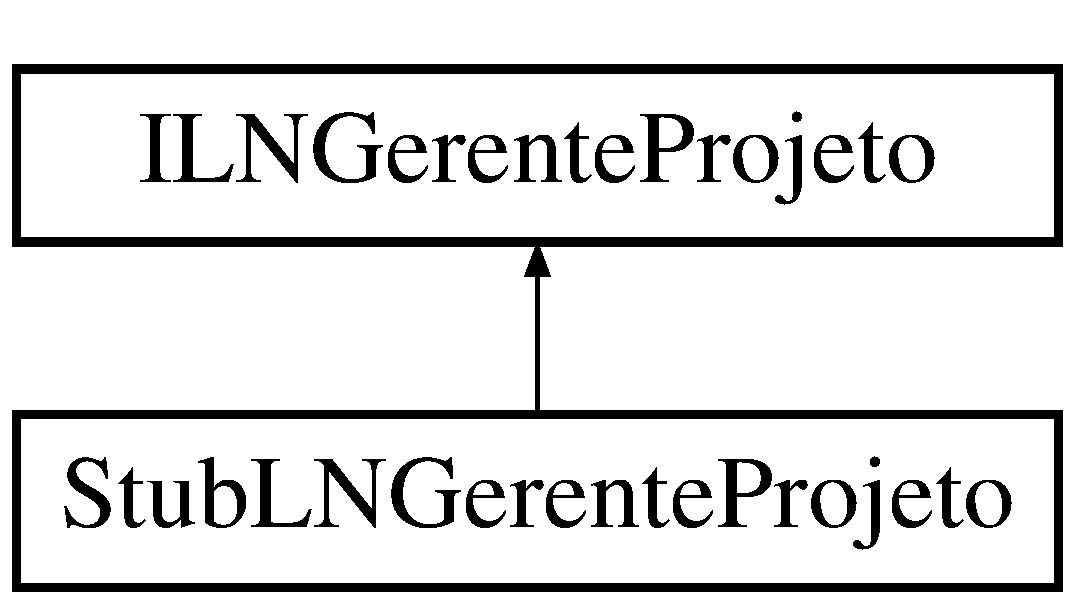
\includegraphics[height=2.000000cm]{class_stub_l_n_gerente_projeto}
\end{center}
\end{figure}
\subsection*{Public Member Functions}
\begin{DoxyCompactItemize}
\item 
\hypertarget{class_stub_l_n_gerente_projeto_acad032e088daca7a2dd70c8c54e5a436}{}\label{class_stub_l_n_gerente_projeto_acad032e088daca7a2dd70c8c54e5a436} 
\hyperlink{class_resultado_gerente_projeto}{Resultado\+Gerente\+Projeto} {\bfseries incluir} (const \hyperlink{class_gerente_projeto}{Gerente\+Projeto} \&)  throw (runtime\+\_\+error)
\item 
\hypertarget{class_stub_l_n_gerente_projeto_af23b547480e51c5ee8f9e8d610ece8d1}{}\label{class_stub_l_n_gerente_projeto_af23b547480e51c5ee8f9e8d610ece8d1} 
\hyperlink{class_resultado_gerente_projeto}{Resultado\+Gerente\+Projeto} {\bfseries remover} (const \hyperlink{class_matricula}{Matricula} \&)  throw (runtime\+\_\+error)
\item 
\hypertarget{class_stub_l_n_gerente_projeto_ab199d8c16488b50c0e21d2132a118250}{}\label{class_stub_l_n_gerente_projeto_ab199d8c16488b50c0e21d2132a118250} 
\hyperlink{class_resultado_gerente_projeto}{Resultado\+Gerente\+Projeto} {\bfseries pesquisar} (const \hyperlink{class_matricula}{Matricula} \&)  throw (runtime\+\_\+error)
\item 
\hypertarget{class_stub_l_n_gerente_projeto_a26bc9351a0785670dac4b77b6aa3e9a9}{}\label{class_stub_l_n_gerente_projeto_a26bc9351a0785670dac4b77b6aa3e9a9} 
\hyperlink{class_resultado_gerente_projeto}{Resultado\+Gerente\+Projeto} {\bfseries editar} (const \hyperlink{class_gerente_projeto}{Gerente\+Projeto} \&)  throw (runtime\+\_\+error)
\end{DoxyCompactItemize}


The documentation for this class was generated from the following file\+:\begin{DoxyCompactItemize}
\item 
\hyperlink{_stubs_8h}{Stubs.\+h}\end{DoxyCompactItemize}

\hypertarget{class_stub_l_n_gerente_sistema}{}\section{Stub\+L\+N\+Gerente\+Sistema Class Reference}
\label{class_stub_l_n_gerente_sistema}\index{Stub\+L\+N\+Gerente\+Sistema@{Stub\+L\+N\+Gerente\+Sistema}}
Inheritance diagram for Stub\+L\+N\+Gerente\+Sistema\+:\begin{figure}[H]
\begin{center}
\leavevmode
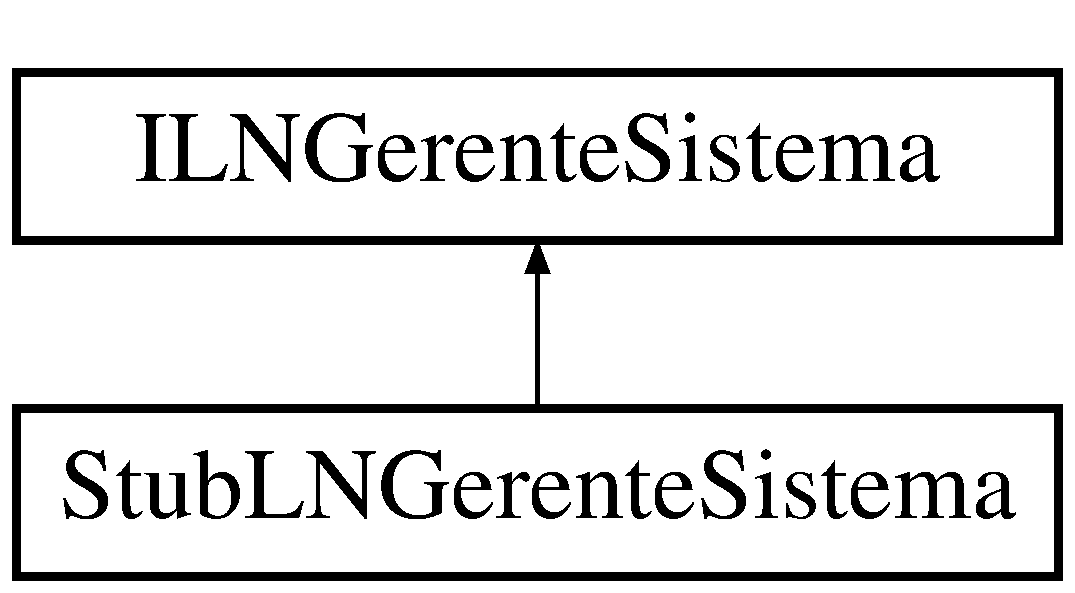
\includegraphics[height=2.000000cm]{class_stub_l_n_gerente_sistema}
\end{center}
\end{figure}
\subsection*{Public Member Functions}
\begin{DoxyCompactItemize}
\item 
\hypertarget{class_stub_l_n_gerente_sistema_ae15fe8bc3171fa9ba4f3d64ba2ea55b5}{}\label{class_stub_l_n_gerente_sistema_ae15fe8bc3171fa9ba4f3d64ba2ea55b5} 
\hyperlink{class_resultado_gerente_sistema}{Resultado\+Gerente\+Sistema} {\bfseries incluir} (const \hyperlink{class_gerente_sistema}{Gerente\+Sistema} \&)  throw (runtime\+\_\+error)
\item 
\hypertarget{class_stub_l_n_gerente_sistema_ab47881f2957822719484bf644188c4d7}{}\label{class_stub_l_n_gerente_sistema_ab47881f2957822719484bf644188c4d7} 
\hyperlink{class_resultado_gerente_sistema}{Resultado\+Gerente\+Sistema} {\bfseries remover} (const \hyperlink{class_matricula}{Matricula} \&)  throw (runtime\+\_\+error)
\item 
\hypertarget{class_stub_l_n_gerente_sistema_a46b09796c8f560fee66491a2b1b0b52b}{}\label{class_stub_l_n_gerente_sistema_a46b09796c8f560fee66491a2b1b0b52b} 
\hyperlink{class_resultado_gerente_sistema}{Resultado\+Gerente\+Sistema} {\bfseries pesquisar} (const \hyperlink{class_matricula}{Matricula} \&)  throw (runtime\+\_\+error)
\item 
\hypertarget{class_stub_l_n_gerente_sistema_ae42d596e2be82d27d06b2024dba1fb0d}{}\label{class_stub_l_n_gerente_sistema_ae42d596e2be82d27d06b2024dba1fb0d} 
\hyperlink{class_resultado_gerente_sistema}{Resultado\+Gerente\+Sistema} {\bfseries editar} (const \hyperlink{class_gerente_sistema}{Gerente\+Sistema} \&)  throw (runtime\+\_\+error)
\end{DoxyCompactItemize}


The documentation for this class was generated from the following file\+:\begin{DoxyCompactItemize}
\item 
\hyperlink{_stubs_8h}{Stubs.\+h}\end{DoxyCompactItemize}

\hypertarget{class_stub_l_n_projeto}{}\section{Stub\+L\+N\+Projeto Class Reference}
\label{class_stub_l_n_projeto}\index{Stub\+L\+N\+Projeto@{Stub\+L\+N\+Projeto}}


Classe que cont�m os m�todos dos stubs de projeto.  




{\ttfamily \#include $<$Stubs.\+h$>$}

Inheritance diagram for Stub\+L\+N\+Projeto\+:\begin{figure}[H]
\begin{center}
\leavevmode
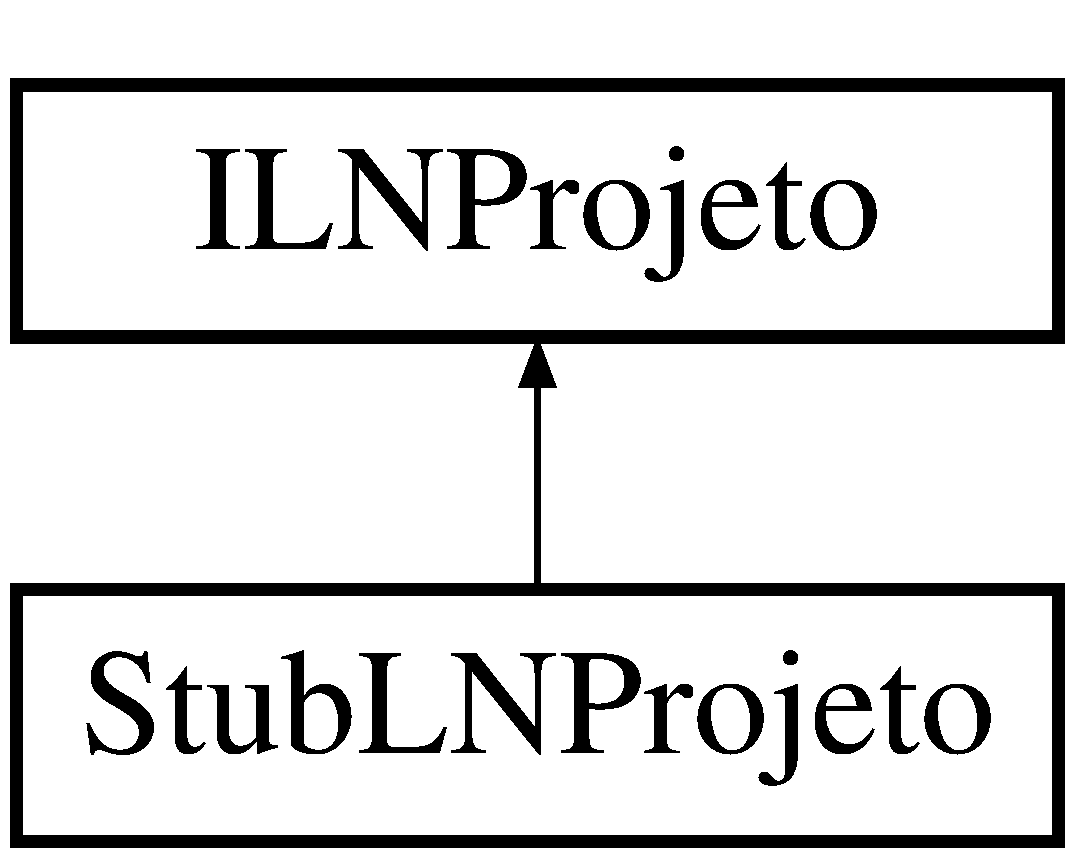
\includegraphics[height=2.000000cm]{class_stub_l_n_projeto}
\end{center}
\end{figure}
\subsection*{Public Member Functions}
\begin{DoxyCompactItemize}
\item 
\hypertarget{class_stub_l_n_projeto_a01e289568494e1344b50f150073ccf67}{}\label{class_stub_l_n_projeto_a01e289568494e1344b50f150073ccf67} 
\hyperlink{class_resultado_projeto}{Resultado\+Projeto} {\bfseries incluir} (const \hyperlink{class_projeto}{Projeto} \&)  throw (runtime\+\_\+error)
\item 
\hypertarget{class_stub_l_n_projeto_a3aad20c048585012ccf7ec10a1ddfbb0}{}\label{class_stub_l_n_projeto_a3aad20c048585012ccf7ec10a1ddfbb0} 
\hyperlink{class_resultado_projeto}{Resultado\+Projeto} {\bfseries remover} (const \hyperlink{class_codigo_projeto}{Codigo\+Projeto} \&)  throw (runtime\+\_\+error)
\item 
\hypertarget{class_stub_l_n_projeto_a58c7f6a301c71a8408b403322394b78a}{}\label{class_stub_l_n_projeto_a58c7f6a301c71a8408b403322394b78a} 
\hyperlink{class_resultado_projeto}{Resultado\+Projeto} {\bfseries pesquisar} (const \hyperlink{class_codigo_projeto}{Codigo\+Projeto} \&)  throw (runtime\+\_\+error)
\item 
\hypertarget{class_stub_l_n_projeto_aa29a5458a06414af40c689527f995484}{}\label{class_stub_l_n_projeto_aa29a5458a06414af40c689527f995484} 
\hyperlink{class_resultado_projeto}{Resultado\+Projeto} {\bfseries editar} (const \hyperlink{class_projeto}{Projeto} \&)  throw (runtime\+\_\+error)
\end{DoxyCompactItemize}


\subsection{Detailed Description}
Classe que cont�m os m�todos dos stubs de projeto. 

Cont�m os prot�tipos dos m�todos da classe de stub referente ao projeto da logica de negocio. 

The documentation for this class was generated from the following file\+:\begin{DoxyCompactItemize}
\item 
\hyperlink{_stubs_8h}{Stubs.\+h}\end{DoxyCompactItemize}

\hypertarget{class_stub_persistencia}{}\section{Stub\+Persistencia Class Reference}
\label{class_stub_persistencia}\index{Stub\+Persistencia@{Stub\+Persistencia}}


Classe que cont�m os m�todos dos stubs de persistencia.  




{\ttfamily \#include $<$Stubs.\+h$>$}

Inheritance diagram for Stub\+Persistencia\+:\begin{figure}[H]
\begin{center}
\leavevmode
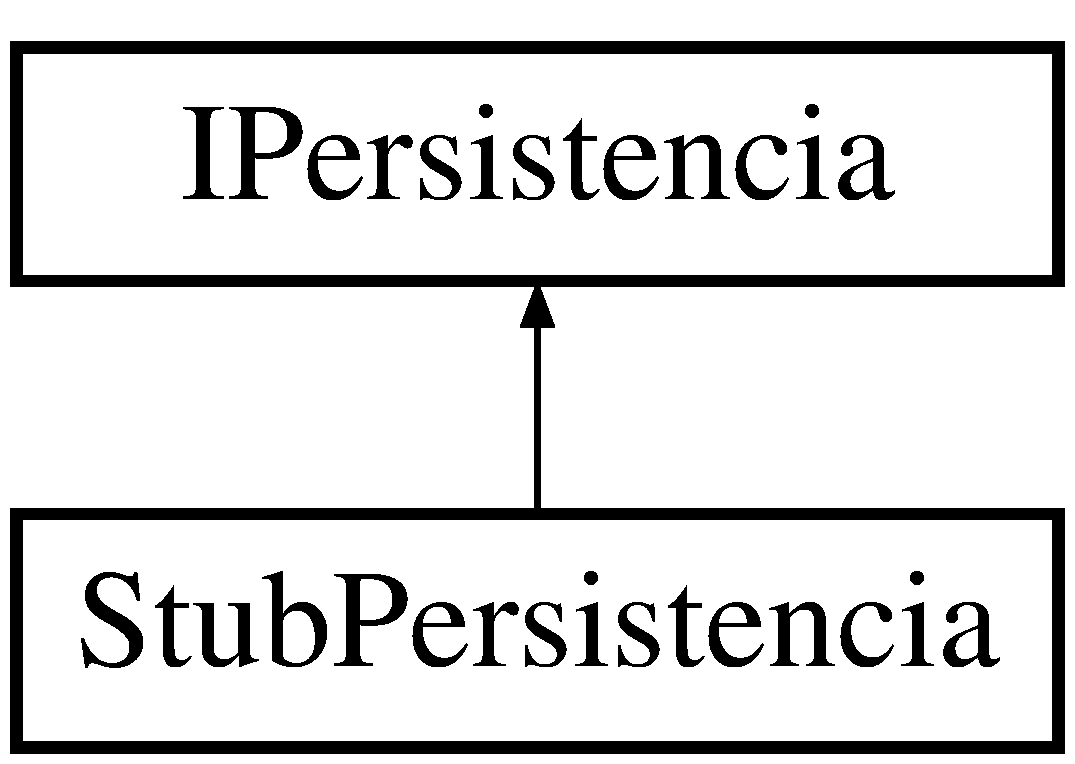
\includegraphics[height=2.000000cm]{class_stub_persistencia}
\end{center}
\end{figure}
\subsection*{Public Member Functions}
\begin{DoxyCompactItemize}
\item 
\hypertarget{class_stub_persistencia_a46ae9f5a8abcbbfa6129dea1761aa9ba}{}\label{class_stub_persistencia_a46ae9f5a8abcbbfa6129dea1761aa9ba} 
void {\bfseries executar} (const \hyperlink{class_comando_banco_dados}{Comando\+Banco\+Dados} $\ast$)  throw (runtime\+\_\+error)
\end{DoxyCompactItemize}


\subsection{Detailed Description}
Classe que cont�m os m�todos dos stubs de persistencia. 

Cont�m os prot�tipos dos m�todos da classe de stub referente a persistencia da logica de negocio. 

The documentation for this class was generated from the following file\+:\begin{DoxyCompactItemize}
\item 
\hyperlink{_stubs_8h}{Stubs.\+h}\end{DoxyCompactItemize}

\hypertarget{class_telefone}{}\section{Telefone Class Reference}
\label{class_telefone}\index{Telefone@{Telefone}}


Classe que cont�m os principais m�todos do telefone do dominio.  




{\ttfamily \#include $<$Dominio.\+h$>$}

\subsection*{Public Member Functions}
\begin{DoxyCompactItemize}
\item 
\hypertarget{class_telefone_a0e07636a72110b0f74bd92c07a25dcce}{}\label{class_telefone_a0e07636a72110b0f74bd92c07a25dcce} 
{\bfseries Telefone} (string)
\item 
\hypertarget{class_telefone_a79516b37434ff927bd2a9bd66080a36d}{}\label{class_telefone_a79516b37434ff927bd2a9bd66080a36d} 
void {\bfseries set\+Telefone} (string)  throw (invalid\+\_\+argument)
\item 
\hypertarget{class_telefone_a64d1e99657fde65bb698ddcd56e7eb04}{}\label{class_telefone_a64d1e99657fde65bb698ddcd56e7eb04} 
string {\bfseries get\+Telefone} () const
\item 
\hypertarget{class_telefone_ae17f36b979bae5118f9f124dbc524e47}{}\label{class_telefone_ae17f36b979bae5118f9f124dbc524e47} 
void {\bfseries is\+Telefone\+Valid} (string)  throw (invalid\+\_\+argument)
\end{DoxyCompactItemize}


\subsection{Detailed Description}
Classe que cont�m os principais m�todos do telefone do dominio. 

Cont�m os prot�tipos dos m�todos do nome referente ao dom�nio do sistema. 

The documentation for this class was generated from the following file\+:\begin{DoxyCompactItemize}
\item 
\hyperlink{_dominio_8h}{Dominio.\+h}\end{DoxyCompactItemize}

\hypertarget{class_t_u_codigo_projeto}{}\section{T\+U\+Codigo\+Projeto Class Reference}
\label{class_t_u_codigo_projeto}\index{T\+U\+Codigo\+Projeto@{T\+U\+Codigo\+Projeto}}


Classe que cont�m os testes de unidade do dom�nio\+: \hyperlink{class_codigo_projeto}{Codigo\+Projeto}.  




{\ttfamily \#include $<$Teste\+Unidade.\+h$>$}

\subsection*{Public Member Functions}
\begin{DoxyCompactItemize}
\item 
\hypertarget{class_t_u_codigo_projeto_a3af146c65cfb8cc225be15a447770a1d}{}\label{class_t_u_codigo_projeto_a3af146c65cfb8cc225be15a447770a1d} 
int \hyperlink{class_t_u_codigo_projeto_a3af146c65cfb8cc225be15a447770a1d}{run} ()
\begin{DoxyCompactList}\small\item\em M�todo que inicia o teste de unidade e retorna um valor inteiro indicando sucesso ou falha. \end{DoxyCompactList}\end{DoxyCompactItemize}
\subsection*{Static Public Attributes}
\begin{DoxyCompactItemize}
\item 
\hypertarget{class_t_u_codigo_projeto_a5115eaa2e3332ba63255cd12c3b41ef2}{}\label{class_t_u_codigo_projeto_a5115eaa2e3332ba63255cd12c3b41ef2} 
static const int \hyperlink{class_t_u_codigo_projeto_a5115eaa2e3332ba63255cd12c3b41ef2}{S\+U\+C\+E\+S\+SO}
\begin{DoxyCompactList}\small\item\em Constante �nica da classe que indica sucesso do teste. \end{DoxyCompactList}\item 
\hypertarget{class_t_u_codigo_projeto_aa209a0ad294577c7d87dd98204ba731e}{}\label{class_t_u_codigo_projeto_aa209a0ad294577c7d87dd98204ba731e} 
static const int \hyperlink{class_t_u_codigo_projeto_aa209a0ad294577c7d87dd98204ba731e}{F\+A\+L\+HA}
\begin{DoxyCompactList}\small\item\em Constante �nica da classe que indica falha do teste. \end{DoxyCompactList}\end{DoxyCompactItemize}


\subsection{Detailed Description}
Classe que cont�m os testes de unidade do dom�nio\+: \hyperlink{class_codigo_projeto}{Codigo\+Projeto}. 

Cont�m os prot�tipos dos m�todos utilizados no teste de unidade e os atributos necess�rios a este. 

The documentation for this class was generated from the following file\+:\begin{DoxyCompactItemize}
\item 
\hyperlink{_teste_unidade_8h}{Teste\+Unidade.\+h}\end{DoxyCompactItemize}

\hypertarget{class_t_u_custo}{}\section{T\+U\+Custo Class Reference}
\label{class_t_u_custo}\index{T\+U\+Custo@{T\+U\+Custo}}


Classe que cont�m os testes de unidade do dom�nio\+: \hyperlink{class_custo}{Custo}.  




{\ttfamily \#include $<$Teste\+Unidade.\+h$>$}

\subsection*{Public Member Functions}
\begin{DoxyCompactItemize}
\item 
\hypertarget{class_t_u_custo_a77f3c0b5db5d43e96d668ddc2a1521b0}{}\label{class_t_u_custo_a77f3c0b5db5d43e96d668ddc2a1521b0} 
int \hyperlink{class_t_u_custo_a77f3c0b5db5d43e96d668ddc2a1521b0}{run} ()
\begin{DoxyCompactList}\small\item\em M�todo que inicia o teste de unidade e retorna um valor inteiro indicando sucesso ou falha. \end{DoxyCompactList}\end{DoxyCompactItemize}
\subsection*{Static Public Attributes}
\begin{DoxyCompactItemize}
\item 
\hypertarget{class_t_u_custo_abc8331a9fe0f630f4814786f5673a9fa}{}\label{class_t_u_custo_abc8331a9fe0f630f4814786f5673a9fa} 
static const int \hyperlink{class_t_u_custo_abc8331a9fe0f630f4814786f5673a9fa}{S\+U\+C\+E\+S\+SO}
\begin{DoxyCompactList}\small\item\em Constante �nica da classe que indica sucesso do teste. \end{DoxyCompactList}\item 
\hypertarget{class_t_u_custo_a4a3b74e5d66a4c183c8f3782cd92f72d}{}\label{class_t_u_custo_a4a3b74e5d66a4c183c8f3782cd92f72d} 
static const int \hyperlink{class_t_u_custo_a4a3b74e5d66a4c183c8f3782cd92f72d}{F\+A\+L\+HA}
\begin{DoxyCompactList}\small\item\em Constante unica da classe que indica falha do teste. \end{DoxyCompactList}\end{DoxyCompactItemize}


\subsection{Detailed Description}
Classe que cont�m os testes de unidade do dom�nio\+: \hyperlink{class_custo}{Custo}. 

Cont�m os prot�tipos dos m�todos utilizados no teste de unidade e os atributos necess�rios a este. 

The documentation for this class was generated from the following file\+:\begin{DoxyCompactItemize}
\item 
\hyperlink{_teste_unidade_8h}{Teste\+Unidade.\+h}\end{DoxyCompactItemize}

\hypertarget{class_t_u_data}{}\section{T\+U\+Data Class Reference}
\label{class_t_u_data}\index{T\+U\+Data@{T\+U\+Data}}


Classe que cont�m os testes de unidade do dom�nio\+: \hyperlink{class_data}{Data}.  




{\ttfamily \#include $<$Teste\+Unidade.\+h$>$}

\subsection*{Public Member Functions}
\begin{DoxyCompactItemize}
\item 
\hypertarget{class_t_u_data_a4fd95b821fa6d55bdc82be6f3a3cbef2}{}\label{class_t_u_data_a4fd95b821fa6d55bdc82be6f3a3cbef2} 
int \hyperlink{class_t_u_data_a4fd95b821fa6d55bdc82be6f3a3cbef2}{run} ()
\begin{DoxyCompactList}\small\item\em M�todo que inicia o teste de unidade e retorna um valor inteiro indicando sucesso ou falha. \end{DoxyCompactList}\end{DoxyCompactItemize}
\subsection*{Static Public Attributes}
\begin{DoxyCompactItemize}
\item 
\hypertarget{class_t_u_data_a1cfa620ca9405154b1d1fd493f1bc9c1}{}\label{class_t_u_data_a1cfa620ca9405154b1d1fd493f1bc9c1} 
static const int \hyperlink{class_t_u_data_a1cfa620ca9405154b1d1fd493f1bc9c1}{S\+U\+C\+E\+S\+SO}
\begin{DoxyCompactList}\small\item\em Constante �nica da classe que indica sucesso do teste. \end{DoxyCompactList}\item 
\hypertarget{class_t_u_data_a04c96978c62b2767b422267129058f0d}{}\label{class_t_u_data_a04c96978c62b2767b422267129058f0d} 
static const int \hyperlink{class_t_u_data_a04c96978c62b2767b422267129058f0d}{F\+A\+L\+HA}
\begin{DoxyCompactList}\small\item\em Constante �nica da classe que indica falha do teste. \end{DoxyCompactList}\end{DoxyCompactItemize}


\subsection{Detailed Description}
Classe que cont�m os testes de unidade do dom�nio\+: \hyperlink{class_data}{Data}. 

Cont�m os prot�tipos dos m�todos utilizados no teste de unidade e os atributos necess�rios a este. 

The documentation for this class was generated from the following file\+:\begin{DoxyCompactItemize}
\item 
\hyperlink{_teste_unidade_8h}{Teste\+Unidade.\+h}\end{DoxyCompactItemize}

\hypertarget{class_t_u_email}{}\section{T\+U\+Email Class Reference}
\label{class_t_u_email}\index{T\+U\+Email@{T\+U\+Email}}


Classe que cont�m os testes de unidade do dom�nio\+: \hyperlink{class_email}{Email}.  




{\ttfamily \#include $<$Teste\+Unidade.\+h$>$}

\subsection*{Public Member Functions}
\begin{DoxyCompactItemize}
\item 
\hypertarget{class_t_u_email_a8d43b68b8b80ada3b28d72d35df9a34f}{}\label{class_t_u_email_a8d43b68b8b80ada3b28d72d35df9a34f} 
int \hyperlink{class_t_u_email_a8d43b68b8b80ada3b28d72d35df9a34f}{run} ()
\begin{DoxyCompactList}\small\item\em M�todo que inicia o teste de unidade e retorna um valor inteiro indicando sucesso ou falha. \end{DoxyCompactList}\end{DoxyCompactItemize}
\subsection*{Static Public Attributes}
\begin{DoxyCompactItemize}
\item 
\hypertarget{class_t_u_email_a70303c6ba5fa454f8abdc01aa0293554}{}\label{class_t_u_email_a70303c6ba5fa454f8abdc01aa0293554} 
static const int \hyperlink{class_t_u_email_a70303c6ba5fa454f8abdc01aa0293554}{S\+U\+C\+E\+S\+SO}
\begin{DoxyCompactList}\small\item\em Constante �nica da classe que indica sucesso do teste. \end{DoxyCompactList}\item 
\hypertarget{class_t_u_email_abfdbe4155ba77b29aba48610fd7d4d71}{}\label{class_t_u_email_abfdbe4155ba77b29aba48610fd7d4d71} 
static const int \hyperlink{class_t_u_email_abfdbe4155ba77b29aba48610fd7d4d71}{F\+A\+L\+HA}
\begin{DoxyCompactList}\small\item\em Constante �nica da classe que indica falha do teste. \end{DoxyCompactList}\end{DoxyCompactItemize}


\subsection{Detailed Description}
Classe que cont�m os testes de unidade do dom�nio\+: \hyperlink{class_email}{Email}. 

Cont�m os prot�tipos dos m�todos utilizados no teste de unidade e os atributos necess�rios a este. 

The documentation for this class was generated from the following file\+:\begin{DoxyCompactItemize}
\item 
\hyperlink{_teste_unidade_8h}{Teste\+Unidade.\+h}\end{DoxyCompactItemize}

\hypertarget{class_t_u_estado_projeto}{}\section{T\+U\+Estado\+Projeto Class Reference}
\label{class_t_u_estado_projeto}\index{T\+U\+Estado\+Projeto@{T\+U\+Estado\+Projeto}}


Classe que cont�m os testes de unidade do dom�nio\+: \hyperlink{class_estado_projeto}{Estado\+Projeto}.  




{\ttfamily \#include $<$Teste\+Unidade.\+h$>$}

\subsection*{Public Member Functions}
\begin{DoxyCompactItemize}
\item 
\hypertarget{class_t_u_estado_projeto_a9e78fdf3c6ecaf61a810eceec81cdf42}{}\label{class_t_u_estado_projeto_a9e78fdf3c6ecaf61a810eceec81cdf42} 
int \hyperlink{class_t_u_estado_projeto_a9e78fdf3c6ecaf61a810eceec81cdf42}{run} ()
\begin{DoxyCompactList}\small\item\em M�todo que inicia o teste de unidade e retorna um valor inteiro indicando sucesso ou falha. \end{DoxyCompactList}\end{DoxyCompactItemize}
\subsection*{Static Public Attributes}
\begin{DoxyCompactItemize}
\item 
\hypertarget{class_t_u_estado_projeto_abdda955b185f9894c88dd2ebe1940df6}{}\label{class_t_u_estado_projeto_abdda955b185f9894c88dd2ebe1940df6} 
static const int \hyperlink{class_t_u_estado_projeto_abdda955b185f9894c88dd2ebe1940df6}{S\+U\+C\+E\+S\+SO}
\begin{DoxyCompactList}\small\item\em Constante �nica da classe que indica sucesso do teste. \end{DoxyCompactList}\item 
\hypertarget{class_t_u_estado_projeto_afccfbf287e36fe23ee4dab23677bb5ea}{}\label{class_t_u_estado_projeto_afccfbf287e36fe23ee4dab23677bb5ea} 
static const int \hyperlink{class_t_u_estado_projeto_afccfbf287e36fe23ee4dab23677bb5ea}{F\+A\+L\+HA}
\begin{DoxyCompactList}\small\item\em Constante �nica da classe que indica falha do teste. \end{DoxyCompactList}\end{DoxyCompactItemize}


\subsection{Detailed Description}
Classe que cont�m os testes de unidade do dom�nio\+: \hyperlink{class_estado_projeto}{Estado\+Projeto}. 

Cont�m os prot�tipos dos m�todos utilizados no teste de unidade e os atributos necess�rios a este. 

The documentation for this class was generated from the following file\+:\begin{DoxyCompactItemize}
\item 
\hyperlink{_teste_unidade_8h}{Teste\+Unidade.\+h}\end{DoxyCompactItemize}

\hypertarget{class_t_u_fase}{}\section{T\+U\+Fase Class Reference}
\label{class_t_u_fase}\index{T\+U\+Fase@{T\+U\+Fase}}


Classe que cont�m os testes de unidade do dom�nio\+: \hyperlink{class_fase}{Fase}.  




{\ttfamily \#include $<$Teste\+Unidade.\+h$>$}

\subsection*{Public Member Functions}
\begin{DoxyCompactItemize}
\item 
\hypertarget{class_t_u_fase_ae042ee7e65da2a7086a34cbdc28edae0}{}\label{class_t_u_fase_ae042ee7e65da2a7086a34cbdc28edae0} 
int \hyperlink{class_t_u_fase_ae042ee7e65da2a7086a34cbdc28edae0}{run} ()
\begin{DoxyCompactList}\small\item\em M�todo que inicia o teste de unidade e retorna um valor inteiro indicando sucesso ou falha. \end{DoxyCompactList}\end{DoxyCompactItemize}
\subsection*{Static Public Attributes}
\begin{DoxyCompactItemize}
\item 
\hypertarget{class_t_u_fase_a864d3913bfe1cc09f51495997082ce2a}{}\label{class_t_u_fase_a864d3913bfe1cc09f51495997082ce2a} 
static const int \hyperlink{class_t_u_fase_a864d3913bfe1cc09f51495997082ce2a}{S\+U\+C\+E\+S\+SO}
\begin{DoxyCompactList}\small\item\em Constante �nica da classe que indica sucesso do teste. \end{DoxyCompactList}\item 
\hypertarget{class_t_u_fase_a937a4a5ad16da4c006df3be5ca434be1}{}\label{class_t_u_fase_a937a4a5ad16da4c006df3be5ca434be1} 
static const int \hyperlink{class_t_u_fase_a937a4a5ad16da4c006df3be5ca434be1}{F\+A\+L\+HA}
\begin{DoxyCompactList}\small\item\em Constante �nica da classe que indica falha do teste. \end{DoxyCompactList}\end{DoxyCompactItemize}


\subsection{Detailed Description}
Classe que cont�m os testes de unidade do dom�nio\+: \hyperlink{class_fase}{Fase}. 

Cont�m os prot�tipos dos m�todos utilizados no teste de unidade e os atributos necess�rios a este. 

The documentation for this class was generated from the following file\+:\begin{DoxyCompactItemize}
\item 
\hyperlink{_teste_unidade_8h}{Teste\+Unidade.\+h}\end{DoxyCompactItemize}

\hypertarget{class_t_u_funcao}{}\section{T\+U\+Funcao Class Reference}
\label{class_t_u_funcao}\index{T\+U\+Funcao@{T\+U\+Funcao}}


Classe que cont�m os testes de unidade do dom�nio\+: \hyperlink{class_funcao}{Funcao}.  




{\ttfamily \#include $<$Teste\+Unidade.\+h$>$}

\subsection*{Public Member Functions}
\begin{DoxyCompactItemize}
\item 
\hypertarget{class_t_u_funcao_a3202c52a69d1c1419295f59c99e4500c}{}\label{class_t_u_funcao_a3202c52a69d1c1419295f59c99e4500c} 
int \hyperlink{class_t_u_funcao_a3202c52a69d1c1419295f59c99e4500c}{run} ()
\begin{DoxyCompactList}\small\item\em M�todo que inicia o teste de unidade e retorna um valor inteiro indicando sucesso ou falha. \end{DoxyCompactList}\end{DoxyCompactItemize}
\subsection*{Static Public Attributes}
\begin{DoxyCompactItemize}
\item 
\hypertarget{class_t_u_funcao_a94c17e3819b3a492a819ce786783fe8d}{}\label{class_t_u_funcao_a94c17e3819b3a492a819ce786783fe8d} 
static const int \hyperlink{class_t_u_funcao_a94c17e3819b3a492a819ce786783fe8d}{S\+U\+C\+E\+S\+SO}
\begin{DoxyCompactList}\small\item\em Constante �nica da classe que indica sucesso do teste. \end{DoxyCompactList}\item 
\hypertarget{class_t_u_funcao_ae07c39f374a900aff707f296a43adc91}{}\label{class_t_u_funcao_ae07c39f374a900aff707f296a43adc91} 
static const int \hyperlink{class_t_u_funcao_ae07c39f374a900aff707f296a43adc91}{F\+A\+L\+HA}
\begin{DoxyCompactList}\small\item\em Constante �nica da classe que indica falha do teste. \end{DoxyCompactList}\end{DoxyCompactItemize}


\subsection{Detailed Description}
Classe que cont�m os testes de unidade do dom�nio\+: \hyperlink{class_funcao}{Funcao}. 

Cont�m os prot�tipos dos m�todos utilizados no teste de unidade e os atributos necess�rios a este. 

The documentation for this class was generated from the following file\+:\begin{DoxyCompactItemize}
\item 
\hyperlink{_teste_unidade_8h}{Teste\+Unidade.\+h}\end{DoxyCompactItemize}

\hypertarget{class_t_u_matricula}{}\section{T\+U\+Matricula Class Reference}
\label{class_t_u_matricula}\index{T\+U\+Matricula@{T\+U\+Matricula}}


Classe que cont�m os testes de unidade do dom�nio\+: \hyperlink{class_matricula}{Matricula}.  




{\ttfamily \#include $<$Teste\+Unidade.\+h$>$}

\subsection*{Public Member Functions}
\begin{DoxyCompactItemize}
\item 
\hypertarget{class_t_u_matricula_a415f6c2f19be6cb4db4f4e61525e56c6}{}\label{class_t_u_matricula_a415f6c2f19be6cb4db4f4e61525e56c6} 
int \hyperlink{class_t_u_matricula_a415f6c2f19be6cb4db4f4e61525e56c6}{run} ()
\begin{DoxyCompactList}\small\item\em M�todo que inicia o teste de unidade e retorna um valor inteiro indicando sucesso ou falha. \end{DoxyCompactList}\end{DoxyCompactItemize}
\subsection*{Static Public Attributes}
\begin{DoxyCompactItemize}
\item 
\hypertarget{class_t_u_matricula_ace940ce9d5f102eb3ab4215b8d421330}{}\label{class_t_u_matricula_ace940ce9d5f102eb3ab4215b8d421330} 
static const string {\bfseries V\+A\+L\+O\+R\+\_\+\+V\+A\+L\+I\+DO}
\item 
\hypertarget{class_t_u_matricula_a212f1bd0f151f47d73b1554f100810ee}{}\label{class_t_u_matricula_a212f1bd0f151f47d73b1554f100810ee} 
static const string {\bfseries V\+A\+L\+O\+R\+\_\+\+I\+N\+V\+A\+L\+I\+DO}
\item 
\hypertarget{class_t_u_matricula_ad39871eb47fc103600d56512b3ea5fbb}{}\label{class_t_u_matricula_ad39871eb47fc103600d56512b3ea5fbb} 
static const int \hyperlink{class_t_u_matricula_ad39871eb47fc103600d56512b3ea5fbb}{S\+U\+C\+E\+S\+SO}
\begin{DoxyCompactList}\small\item\em Constante �nica da classe que indica sucesso do teste. \end{DoxyCompactList}\item 
\hypertarget{class_t_u_matricula_a9fd88e540691a0f1eccec436af1b6574}{}\label{class_t_u_matricula_a9fd88e540691a0f1eccec436af1b6574} 
static const int \hyperlink{class_t_u_matricula_a9fd88e540691a0f1eccec436af1b6574}{F\+A\+L\+HA}
\begin{DoxyCompactList}\small\item\em Constante �nica da classe que indica falha do teste. \end{DoxyCompactList}\end{DoxyCompactItemize}


\subsection{Detailed Description}
Classe que cont�m os testes de unidade do dom�nio\+: \hyperlink{class_matricula}{Matricula}. 

Cont�m os prot�tipos dos m�todos utilizados no teste de unidade e os atributos necess�rios a este. 

The documentation for this class was generated from the following file\+:\begin{DoxyCompactItemize}
\item 
\hyperlink{_teste_unidade_8h}{Teste\+Unidade.\+h}\end{DoxyCompactItemize}

\hypertarget{class_t_u_nome}{}\section{T\+U\+Nome Class Reference}
\label{class_t_u_nome}\index{T\+U\+Nome@{T\+U\+Nome}}


Classe que cont�m os testes de unidade do dom�nio\+: \hyperlink{class_nome}{Nome}.  




{\ttfamily \#include $<$Teste\+Unidade.\+h$>$}

\subsection*{Public Member Functions}
\begin{DoxyCompactItemize}
\item 
\hypertarget{class_t_u_nome_ae20734cb15f71890e57aff02a00f6313}{}\label{class_t_u_nome_ae20734cb15f71890e57aff02a00f6313} 
int \hyperlink{class_t_u_nome_ae20734cb15f71890e57aff02a00f6313}{run} ()
\begin{DoxyCompactList}\small\item\em M�todo que inicia o teste de unidade e retorna um valor inteiro indicando sucesso ou falha. \end{DoxyCompactList}\end{DoxyCompactItemize}
\subsection*{Static Public Attributes}
\begin{DoxyCompactItemize}
\item 
\hypertarget{class_t_u_nome_af58123c3e8b9d8523c01820ac9ca5054}{}\label{class_t_u_nome_af58123c3e8b9d8523c01820ac9ca5054} 
static const int \hyperlink{class_t_u_nome_af58123c3e8b9d8523c01820ac9ca5054}{S\+U\+C\+E\+S\+SO}
\begin{DoxyCompactList}\small\item\em Constante �nica da classe que indica sucesso do teste. \end{DoxyCompactList}\item 
\hypertarget{class_t_u_nome_a21b319a9928694baf5675aaf266f357a}{}\label{class_t_u_nome_a21b319a9928694baf5675aaf266f357a} 
static const int \hyperlink{class_t_u_nome_a21b319a9928694baf5675aaf266f357a}{F\+A\+L\+HA}
\begin{DoxyCompactList}\small\item\em Constante �nica da classe que indica falha do teste. \end{DoxyCompactList}\end{DoxyCompactItemize}


\subsection{Detailed Description}
Classe que cont�m os testes de unidade do dom�nio\+: \hyperlink{class_nome}{Nome}. 

Cont�m os prot�tipos dos m�todos utilizados no teste de unidade e os atributos necess�rios a este. 

The documentation for this class was generated from the following file\+:\begin{DoxyCompactItemize}
\item 
\hyperlink{_teste_unidade_8h}{Teste\+Unidade.\+h}\end{DoxyCompactItemize}

\hypertarget{class_t_u_senha}{}\section{T\+U\+Senha Class Reference}
\label{class_t_u_senha}\index{T\+U\+Senha@{T\+U\+Senha}}


Classe que cont�m os testes de unidade do dom�nio\+: \hyperlink{class_senha}{Senha}.  




{\ttfamily \#include $<$Teste\+Unidade.\+h$>$}

\subsection*{Public Member Functions}
\begin{DoxyCompactItemize}
\item 
\hypertarget{class_t_u_senha_ac5ddea52ed42b828961f343b82074125}{}\label{class_t_u_senha_ac5ddea52ed42b828961f343b82074125} 
int \hyperlink{class_t_u_senha_ac5ddea52ed42b828961f343b82074125}{run} ()
\begin{DoxyCompactList}\small\item\em M�todo que inicia o teste de unidade e retorna um valor inteiro indicando sucesso ou falha. \end{DoxyCompactList}\end{DoxyCompactItemize}
\subsection*{Static Public Attributes}
\begin{DoxyCompactItemize}
\item 
\hypertarget{class_t_u_senha_aabbf4cc53825634e3e5e75af53585eb0}{}\label{class_t_u_senha_aabbf4cc53825634e3e5e75af53585eb0} 
static const string {\bfseries V\+A\+L\+O\+R\+\_\+\+V\+A\+L\+I\+DO}
\item 
\hypertarget{class_t_u_senha_a44683d14808dd5ff285e205a22a54a21}{}\label{class_t_u_senha_a44683d14808dd5ff285e205a22a54a21} 
static const string {\bfseries V\+A\+L\+O\+R\+\_\+\+I\+N\+V\+A\+L\+I\+DO}
\item 
\hypertarget{class_t_u_senha_ab1cbae7c007e371d27ab547afbbc56b8}{}\label{class_t_u_senha_ab1cbae7c007e371d27ab547afbbc56b8} 
static const int \hyperlink{class_t_u_senha_ab1cbae7c007e371d27ab547afbbc56b8}{S\+U\+C\+E\+S\+SO}
\begin{DoxyCompactList}\small\item\em Constante �nica da classe que indica sucesso do teste. \end{DoxyCompactList}\item 
\hypertarget{class_t_u_senha_a7c766c0120cc65921af91c31c56babc1}{}\label{class_t_u_senha_a7c766c0120cc65921af91c31c56babc1} 
static const int \hyperlink{class_t_u_senha_a7c766c0120cc65921af91c31c56babc1}{F\+A\+L\+HA}
\begin{DoxyCompactList}\small\item\em Constante �nica da classe que indica falha do teste. \end{DoxyCompactList}\end{DoxyCompactItemize}


\subsection{Detailed Description}
Classe que cont�m os testes de unidade do dom�nio\+: \hyperlink{class_senha}{Senha}. 

Cont�m os prot�tipos dos m�todos utilizados no teste de unidade e os atributos necess�rios a este. 

The documentation for this class was generated from the following file\+:\begin{DoxyCompactItemize}
\item 
\hyperlink{_teste_unidade_8h}{Teste\+Unidade.\+h}\end{DoxyCompactItemize}

\hypertarget{class_t_u_telefone}{}\section{T\+U\+Telefone Class Reference}
\label{class_t_u_telefone}\index{T\+U\+Telefone@{T\+U\+Telefone}}


Classe que cont�m os testes de unidade do dom�nio\+: \hyperlink{class_telefone}{Telefone}.  




{\ttfamily \#include $<$Teste\+Unidade.\+h$>$}

\subsection*{Public Member Functions}
\begin{DoxyCompactItemize}
\item 
\hypertarget{class_t_u_telefone_abdf98e48a737ab44ad59cc63f26d6788}{}\label{class_t_u_telefone_abdf98e48a737ab44ad59cc63f26d6788} 
int \hyperlink{class_t_u_telefone_abdf98e48a737ab44ad59cc63f26d6788}{run} ()
\begin{DoxyCompactList}\small\item\em M�todo que inicia o teste de unidade e retorna um valor inteiro indicando sucesso ou falha. \end{DoxyCompactList}\end{DoxyCompactItemize}
\subsection*{Static Public Attributes}
\begin{DoxyCompactItemize}
\item 
\hypertarget{class_t_u_telefone_a30c829e85a3182c39588498bc6447ec1}{}\label{class_t_u_telefone_a30c829e85a3182c39588498bc6447ec1} 
static const int \hyperlink{class_t_u_telefone_a30c829e85a3182c39588498bc6447ec1}{S\+U\+C\+E\+S\+SO}
\begin{DoxyCompactList}\small\item\em Constante �nica da classe que indica sucesso do teste. \end{DoxyCompactList}\item 
\hypertarget{class_t_u_telefone_ac724a744fe43bf8c04108a7b98925a2d}{}\label{class_t_u_telefone_ac724a744fe43bf8c04108a7b98925a2d} 
static const int \hyperlink{class_t_u_telefone_ac724a744fe43bf8c04108a7b98925a2d}{F\+A\+L\+HA}
\begin{DoxyCompactList}\small\item\em Constante �nica da classe que indica falha do teste. \end{DoxyCompactList}\end{DoxyCompactItemize}


\subsection{Detailed Description}
Classe que cont�m os testes de unidade do dom�nio\+: \hyperlink{class_telefone}{Telefone}. 

Cont�m os prot�tipos dos m�todos utilizados no teste de unidade e os atributos necess�rios a este. 

The documentation for this class was generated from the following file\+:\begin{DoxyCompactItemize}
\item 
\hyperlink{_teste_unidade_8h}{Teste\+Unidade.\+h}\end{DoxyCompactItemize}

\hypertarget{class_usuario}{}\section{Usuario Class Reference}
\label{class_usuario}\index{Usuario@{Usuario}}


Classe que cont�m os principais m�todos da entidade de usu�rio.  




{\ttfamily \#include $<$Entidade.\+h$>$}

Inheritance diagram for Usuario\+:\begin{figure}[H]
\begin{center}
\leavevmode
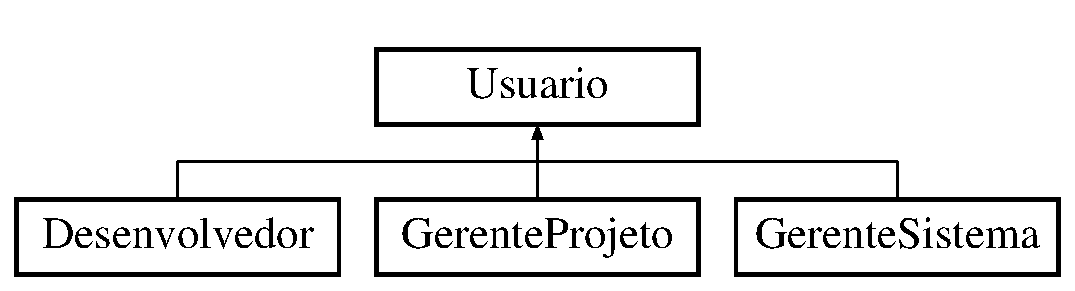
\includegraphics[height=2.000000cm]{class_usuario}
\end{center}
\end{figure}
\subsection*{Public Member Functions}
\begin{DoxyCompactItemize}
\item 
\hypertarget{class_usuario_a93e0f77d77c68c441fbcf433b0cec8bd}{}\label{class_usuario_a93e0f77d77c68c441fbcf433b0cec8bd} 
{\bfseries Usuario} (\hyperlink{class_nome}{Nome}, \hyperlink{class_matricula}{Matricula}, \hyperlink{class_senha}{Senha})
\end{DoxyCompactItemize}
\subsection*{Public Attributes}
\begin{DoxyCompactItemize}
\item 
\hypertarget{class_usuario_ae3b5cc7679c123d260dea72876b7bc26}{}\label{class_usuario_ae3b5cc7679c123d260dea72876b7bc26} 
\hyperlink{class_nome}{Nome} {\bfseries nome}
\item 
\hypertarget{class_usuario_af86c92a7f40d89b246e4024103ea60c2}{}\label{class_usuario_af86c92a7f40d89b246e4024103ea60c2} 
\hyperlink{class_matricula}{Matricula} {\bfseries matricula}
\item 
\hypertarget{class_usuario_ac53101cd72b76334475d2a6258b7190e}{}\label{class_usuario_ac53101cd72b76334475d2a6258b7190e} 
\hyperlink{class_senha}{Senha} {\bfseries senha}
\item 
\hypertarget{class_usuario_a300ab4bb7527f14d687fa1ba7b36c8ba}{}\label{class_usuario_a300ab4bb7527f14d687fa1ba7b36c8ba} 
\hyperlink{class_funcao}{Funcao} {\bfseries funcao}
\end{DoxyCompactItemize}


\subsection{Detailed Description}
Classe que cont�m os principais m�todos da entidade de usu�rio. 

Cont�m os prot�tipos dos m�todos da classe usu�rio referente �s entidades do sistema que serao herdadas de outras classes. 

The documentation for this class was generated from the following file\+:\begin{DoxyCompactItemize}
\item 
\hyperlink{_entidade_8h}{Entidade.\+h}\end{DoxyCompactItemize}

\chapter{File Documentation}
\hypertarget{_builders_8h}{}\section{Builders.\+h File Reference}
\label{_builders_8h}\index{Builders.\+h@{Builders.\+h}}


Arquivo que cont�m as classes construtoras dos objetos do sistema.  


{\ttfamily \#include \char`\"{}Interfaces.\+h\char`\"{}}\newline
{\ttfamily \#include \char`\"{}Dominio.\+h\char`\"{}}\newline
{\ttfamily \#include \char`\"{}Controladoras.\+h\char`\"{}}\newline
{\ttfamily \#include \char`\"{}Stubs.\+h\char`\"{}}\newline
{\ttfamily \#include $<$stdexcept$>$}\newline
{\ttfamily \#include $<$iostream$>$}\newline
{\ttfamily \#include $<$cstdlib$>$}\newline
\subsection*{Classes}
\begin{DoxyCompactItemize}
\item 
class \hyperlink{class_builder_subsistema_gerente_projeto_teste}{Builder\+Subsistema\+Gerente\+Projeto\+Teste}
\begin{DoxyCompactList}\small\item\em Classe respons�vel por testar o construtor de Gerente de \hyperlink{class_projeto}{Projeto} na interface. \end{DoxyCompactList}\item 
class \hyperlink{class_builder_subsistema_gerente_sistema_teste}{Builder\+Subsistema\+Gerente\+Sistema\+Teste}
\begin{DoxyCompactList}\small\item\em Classe respons�vel por testar o construtor de Gerente de Sistema na interface. \end{DoxyCompactList}\item 
class \hyperlink{class_builder_subsistema_projeto_teste}{Builder\+Subsistema\+Projeto\+Teste}
\begin{DoxyCompactList}\small\item\em Classe respons�vel por testar o construtor de \hyperlink{class_projeto}{Projeto} na interface. \end{DoxyCompactList}\item 
class \hyperlink{class_builder_subsistema_desenvolvedor_teste}{Builder\+Subsistema\+Desenvolvedor\+Teste}
\begin{DoxyCompactList}\small\item\em Classe respons�vel por testar o construtor de \hyperlink{class_desenvolvedor}{Desenvolvedor} na interface. \end{DoxyCompactList}\end{DoxyCompactItemize}


\subsection{Detailed Description}
Arquivo que cont�m as classes construtoras dos objetos do sistema. 

O arquivo \hyperlink{_builders_8h}{Builders.\+h} cont�m os prot�tipos de todas as classes construturas que permitem a cria��o dos objetos do sistema. 
\hypertarget{_comandos_8h}{}\section{Comandos.\+h File Reference}
\label{_comandos_8h}\index{Comandos.\+h@{Comandos.\+h}}


Arquivo que contém as classes do módulo de lógica de negócio.  


\subsection*{Classes}
\begin{DoxyCompactItemize}
\item 
class \hyperlink{class_comando_banco_dados}{Comando\+Banco\+Dados}
\begin{DoxyCompactList}\small\item\em Classe que contém os principais métodos dos comandos do banco de dados. \end{DoxyCompactList}\item 
class \hyperlink{class_comando_incluir_gerente_projeto}{Comando\+Incluir\+Gerente\+Projeto}
\begin{DoxyCompactList}\small\item\em Classe responsável por\+: Incluir Gerente de projeto. \end{DoxyCompactList}\item 
class \hyperlink{class_comando_remover_gerente_projeto}{Comando\+Remover\+Gerente\+Projeto}
\begin{DoxyCompactList}\small\item\em Classe responsável por\+: Remover Gerente de projeto. \end{DoxyCompactList}\item 
class \hyperlink{class_comando_recuperar_gerente_projeto}{Comando\+Recuperar\+Gerente\+Projeto}
\begin{DoxyCompactList}\small\item\em Classe responsável por\+: Recuperar Gerente de projeto. \end{DoxyCompactList}\item 
class \hyperlink{class_comando_editar_gerente_projeto}{Comando\+Editar\+Gerente\+Projeto}
\begin{DoxyCompactList}\small\item\em Classe responsável por\+: Editar Gerente de projeto. \end{DoxyCompactList}\item 
class \hyperlink{class_comando_incluir_gerente_sistema}{Comando\+Incluir\+Gerente\+Sistema}
\begin{DoxyCompactList}\small\item\em Classe responsável por\+: Incluir Gerente de sistema. \end{DoxyCompactList}\item 
class \hyperlink{class_comando_remover_gerente_sistema}{Comando\+Remover\+Gerente\+Sistema}
\begin{DoxyCompactList}\small\item\em Classe responsável por\+: Remover Gerente de sistema. \end{DoxyCompactList}\item 
class \hyperlink{class_comando_recuperar_gerente_sistema}{Comando\+Recuperar\+Gerente\+Sistema}
\item 
class \hyperlink{class_comando_editar_gerente_sistema}{Comando\+Editar\+Gerente\+Sistema}
\begin{DoxyCompactList}\small\item\em Classe responsável por\+: Editar Gerente de sistema. \end{DoxyCompactList}\item 
class \hyperlink{class_comando_incluir_projeto}{Comando\+Incluir\+Projeto}
\begin{DoxyCompactList}\small\item\em Classe responsável por\+: Incluir projeto. \end{DoxyCompactList}\item 
class \hyperlink{class_comando_remover_projeto}{Comando\+Remover\+Projeto}
\begin{DoxyCompactList}\small\item\em Classe responsável por\+: Remover projeto. \end{DoxyCompactList}\item 
class \hyperlink{class_comando_recuperar_projeto}{Comando\+Recuperar\+Projeto}
\begin{DoxyCompactList}\small\item\em Classe responsável por\+: Recuperar projeto. \end{DoxyCompactList}\item 
class \hyperlink{class_comando_editar_projeto}{Comando\+Editar\+Projeto}
\begin{DoxyCompactList}\small\item\em Classe responsável por\+: Editar projeto. \end{DoxyCompactList}\item 
class \hyperlink{class_comando_incluir_desenvolvedor}{Comando\+Incluir\+Desenvolvedor}
\begin{DoxyCompactList}\small\item\em Classe responsável por\+: Incluir desenvolvedor. \end{DoxyCompactList}\item 
class \hyperlink{class_comando_remover_desenvolvedor}{Comando\+Remover\+Desenvolvedor}
\begin{DoxyCompactList}\small\item\em Classe responsável por\+: Remover desenvolvedor. \end{DoxyCompactList}\item 
class \hyperlink{class_comando_recuperar_desenvolvedor}{Comando\+Recuperar\+Desenvolvedor}
\begin{DoxyCompactList}\small\item\em Classe responsável por\+: Recuperar desenvolvedor. \end{DoxyCompactList}\item 
class \hyperlink{class_comando_editar_desenvolvedor}{Comando\+Editar\+Desenvolvedor}
\begin{DoxyCompactList}\small\item\em Classe responsável por\+: Editar desenvolvedor. \end{DoxyCompactList}\end{DoxyCompactItemize}


\subsection{Detailed Description}
Arquivo que contém as classes do módulo de lógica de negócio. 

O arquivo \hyperlink{_comandos_8h}{Comandos.\+h} contém os protótipos de todas as classes que definem a lógica de negócio referentes ao banco de dados. 
\hypertarget{_controladoras_8h}{}\section{Controladoras.\+h File Reference}
\label{_controladoras_8h}\index{Controladoras.\+h@{Controladoras.\+h}}


Arquivo que cont�m as classes do m�dulo que faz a comunica��o entre a interface com o a l�gica de negocio.  


{\ttfamily \#include \char`\"{}Interfaces.\+h\char`\"{}}\newline
{\ttfamily \#include \char`\"{}Dominio.\+h\char`\"{}}\newline
{\ttfamily \#include $<$stdexcept$>$}\newline
{\ttfamily \#include $<$iostream$>$}\newline
{\ttfamily \#include $<$cstdlib$>$}\newline
\subsection*{Classes}
\begin{DoxyCompactItemize}
\item 
class \hyperlink{class_cntr_i_u_autenticacao}{Cntr\+I\+U\+Autenticacao}
\begin{DoxyCompactList}\small\item\em Classe respons�vel por autentica��o na interface. \end{DoxyCompactList}\item 
class \hyperlink{class_cntr_i_u_projeto}{Cntr\+I\+U\+Projeto}
\begin{DoxyCompactList}\small\item\em Classe respons�vel pelo controle do projeto na interface. \end{DoxyCompactList}\item 
class \hyperlink{class_cntr_i_u_gerente_projeto}{Cntr\+I\+U\+Gerente\+Projeto}
\begin{DoxyCompactList}\small\item\em Classe respons�vel pelo controle do gerente de projeto na interface. \end{DoxyCompactList}\item 
class \hyperlink{class_cntr_i_u_gerente_projeto_1_1_cntr_inclusao}{Cntr\+I\+U\+Gerente\+Projeto\+::\+Cntr\+Inclusao}
\begin{DoxyCompactList}\small\item\em Classe interna respons�vel pela inclus�o do gerente de projeto na interface l�gica de neg�cio. \end{DoxyCompactList}\item 
class \hyperlink{class_cntr_i_u_gerente_projeto_1_1_cntr_remocao}{Cntr\+I\+U\+Gerente\+Projeto\+::\+Cntr\+Remocao}
\begin{DoxyCompactList}\small\item\em Classe interna respons�vel pela remo��o do gerente de projeto na interface l�gica de neg�cio. \end{DoxyCompactList}\item 
class \hyperlink{class_cntr_i_u_gerente_projeto_1_1_cntr_pesquisa}{Cntr\+I\+U\+Gerente\+Projeto\+::\+Cntr\+Pesquisa}
\begin{DoxyCompactList}\small\item\em Classe interna respons�vel pela pesquisa do gerente de projeto na interface l�gica de neg�cio. \end{DoxyCompactList}\item 
class \hyperlink{class_cntr_i_u_gerente_projeto_1_1_cntr_edicao}{Cntr\+I\+U\+Gerente\+Projeto\+::\+Cntr\+Edicao}
\begin{DoxyCompactList}\small\item\em Classe interna respons�vel pela edi��o do gerente de projeto na interface l�gica de neg�cio. \end{DoxyCompactList}\item 
class \hyperlink{class_cntr_i_u_gerente_sistema}{Cntr\+I\+U\+Gerente\+Sistema}
\begin{DoxyCompactList}\small\item\em Classe respons�vel pelo controle do gerente de sistema na interface. \end{DoxyCompactList}\item 
class \hyperlink{class_cntr_i_u_gerente_sistema_1_1_cntr_inclusao}{Cntr\+I\+U\+Gerente\+Sistema\+::\+Cntr\+Inclusao}
\begin{DoxyCompactList}\small\item\em Classe interna respons�vel pela inclus�o do gerente de sistema na interface l�gica de neg�cio. \end{DoxyCompactList}\item 
class \hyperlink{class_cntr_i_u_gerente_sistema_1_1_cntr_remocao}{Cntr\+I\+U\+Gerente\+Sistema\+::\+Cntr\+Remocao}
\begin{DoxyCompactList}\small\item\em Classe interna respons�vel pela remo�ao do gerente de sistema na interface l�gica de neg�cio. \end{DoxyCompactList}\item 
class \hyperlink{class_cntr_i_u_gerente_sistema_1_1_cntr_pesquisa}{Cntr\+I\+U\+Gerente\+Sistema\+::\+Cntr\+Pesquisa}
\begin{DoxyCompactList}\small\item\em Classe interna respons�vel pela pesquisa do gerente de sistema na interface l�gica de neg�cio. \end{DoxyCompactList}\item 
class \hyperlink{class_cntr_i_u_gerente_sistema_1_1_cntr_edicao}{Cntr\+I\+U\+Gerente\+Sistema\+::\+Cntr\+Edicao}
\item 
class \hyperlink{class_cntr_i_u_desenvolvedor}{Cntr\+I\+U\+Desenvolvedor}
\begin{DoxyCompactList}\small\item\em Classe respons�vel pelo controle do desenvolvedor na interface. \end{DoxyCompactList}\end{DoxyCompactItemize}


\subsection{Detailed Description}
Arquivo que cont�m as classes do m�dulo que faz a comunica��o entre a interface com o a l�gica de negocio. 

O arquivo \hyperlink{_controladoras_8h}{Controladoras.\+h} cont�m os prot�tipos de todas as classes que permitem a comunica��o entre a interface de usu�rio e a l�gica de neg�cio. 
\hypertarget{_dominio_8h}{}\section{Dominio.\+h File Reference}
\label{_dominio_8h}\index{Dominio.\+h@{Dominio.\+h}}


Arquivo que cont�m as classes do m�dulo Dom�nio.  


{\ttfamily \#include $<$string$>$}\newline
{\ttfamily \#include $<$stdexcept$>$}\newline
\subsection*{Classes}
\begin{DoxyCompactItemize}
\item 
class \hyperlink{class_nome}{Nome}
\begin{DoxyCompactList}\small\item\em Classe que cont�m os principais m�todos do nome do dominio. \end{DoxyCompactList}\item 
class \hyperlink{class_senha}{Senha}
\begin{DoxyCompactList}\small\item\em Classe que cont�m os principais m�todos da senha do dominio. \end{DoxyCompactList}\item 
class \hyperlink{class_codigo_projeto}{Codigo\+Projeto}
\begin{DoxyCompactList}\small\item\em Classe que cont�m os principais m�todos do codigo do projeto do dominio. \end{DoxyCompactList}\item 
class \hyperlink{class_telefone}{Telefone}
\begin{DoxyCompactList}\small\item\em Classe que cont�m os principais m�todos do telefone do dominio. \end{DoxyCompactList}\item 
class \hyperlink{class_estado_projeto}{Estado\+Projeto}
\begin{DoxyCompactList}\small\item\em Classe que cont�m os principais m�todos do Estado do \hyperlink{class_projeto}{Projeto} do dominio. \end{DoxyCompactList}\item 
class \hyperlink{class_fase}{Fase}
\begin{DoxyCompactList}\small\item\em Classe que cont�m os principais m�todos da fase do dominio. \end{DoxyCompactList}\item 
class \hyperlink{class_funcao}{Funcao}
\begin{DoxyCompactList}\small\item\em Classe que cont�m os principais m�todos da fun��o do dominio. \end{DoxyCompactList}\item 
class \hyperlink{class_matricula}{Matricula}
\begin{DoxyCompactList}\small\item\em Classe que cont�m os principais m�todos da matricula do dominio. \end{DoxyCompactList}\item 
class \hyperlink{class_data}{Data}
\begin{DoxyCompactList}\small\item\em Classe que cont�m os principais m�todos da data do dominio. \end{DoxyCompactList}\item 
class \hyperlink{class_email}{Email}
\begin{DoxyCompactList}\small\item\em Classe que cont�m os principais m�todos do email do dominio. \end{DoxyCompactList}\item 
class \hyperlink{class_custo}{Custo}
\begin{DoxyCompactList}\small\item\em Classe que cont�m os principais m�todos do custo do dominio. \end{DoxyCompactList}\end{DoxyCompactItemize}


\subsection{Detailed Description}
Arquivo que cont�m as classes do m�dulo Dom�nio. 

O arquivo \hyperlink{_dominio_8h}{Dominio.\+h} cont�m os prot�tipos de todas as classes que definem os dom�nios referentes ao sistema. 
\hypertarget{_entidade_8h}{}\section{Entidade.\+h File Reference}
\label{_entidade_8h}\index{Entidade.\+h@{Entidade.\+h}}


Arquivo que cont�m as classes do m�dulo de entidade.  


{\ttfamily \#include $<$string$>$}\newline
{\ttfamily \#include $<$stdexcept$>$}\newline
{\ttfamily \#include \char`\"{}Dominio.\+h\char`\"{}}\newline
\subsection*{Classes}
\begin{DoxyCompactItemize}
\item 
class \hyperlink{class_usuario}{Usuario}
\begin{DoxyCompactList}\small\item\em Classe que cont�m os principais m�todos da entidade de usu�rio. \end{DoxyCompactList}\item 
class \hyperlink{class_desenvolvedor}{Desenvolvedor}
\begin{DoxyCompactList}\small\item\em Classe que cont�m os principais m�todos da entidade de desenvolvedor. \end{DoxyCompactList}\item 
class \hyperlink{class_gerente_projeto}{Gerente\+Projeto}
\begin{DoxyCompactList}\small\item\em Classe que cont�m os principais m�todos da entidade de gerente de projeto. \end{DoxyCompactList}\item 
class \hyperlink{class_gerente_sistema}{Gerente\+Sistema}
\begin{DoxyCompactList}\small\item\em Classe que cont�m os principais m�todos da entidade de gerente de sistema. \end{DoxyCompactList}\item 
class \hyperlink{class_fase_projeto}{Fase\+Projeto}
\begin{DoxyCompactList}\small\item\em Classe que cont�m os principais m�todos da entidade de fase de projeto. \end{DoxyCompactList}\item 
class \hyperlink{class_projeto}{Projeto}
\begin{DoxyCompactList}\small\item\em Classe que cont�m os principais m�todos da entidade de projeto. \end{DoxyCompactList}\item 
class \hyperlink{class_resultado}{Resultado}
\begin{DoxyCompactList}\small\item\em Classe que cont�m os principais m�todos da entidade de \hyperlink{class_resultado}{Resultado}. \end{DoxyCompactList}\item 
class \hyperlink{class_resultado_autenticacao}{Resultado\+Autenticacao}
\begin{DoxyCompactList}\small\item\em Classe que cont�m os principais m�todos da entidade de \hyperlink{class_resultado}{Resultado} de autenticacao. \end{DoxyCompactList}\item 
class \hyperlink{class_resultado_projeto}{Resultado\+Projeto}
\begin{DoxyCompactList}\small\item\em Classe que cont�m os principais m�todos da entidade de \hyperlink{class_resultado}{Resultado} de projeto. \end{DoxyCompactList}\item 
class \hyperlink{class_resultado_gerente_projeto}{Resultado\+Gerente\+Projeto}
\begin{DoxyCompactList}\small\item\em Classe que cont�m os principais m�todos da entidade de \hyperlink{class_resultado}{Resultado} de Gerente de \hyperlink{class_projeto}{Projeto}. \end{DoxyCompactList}\item 
class \hyperlink{class_resultado_gerente_sistema}{Resultado\+Gerente\+Sistema}
\begin{DoxyCompactList}\small\item\em Classe que cont�m os principais m�todos da entidade de resultado de gerente de sistema. \end{DoxyCompactList}\item 
class \hyperlink{class_resultado_desenvolvedor}{Resultado\+Desenvolvedor}
\begin{DoxyCompactList}\small\item\em Classe que cont�m os principais m�todos da entidade de \hyperlink{class_resultado}{Resultado} de desenvolvedor. \end{DoxyCompactList}\end{DoxyCompactItemize}


\subsection{Detailed Description}
Arquivo que cont�m as classes do m�dulo de entidade. 

O arquivo \hyperlink{_entidade_8h}{Entidade.\+h} cont�m os prot�tipos de todas as classes que definem as entidades referentes ao sistema. 
\hypertarget{_interfaces_8h}{}\section{Interfaces.\+h File Reference}
\label{_interfaces_8h}\index{Interfaces.\+h@{Interfaces.\+h}}


Arquivo que contém as classes do módulo de interface.  


{\ttfamily \#include \char`\"{}Dominio.\+h\char`\"{}}\newline
{\ttfamily \#include \char`\"{}Entidade.\+h\char`\"{}}\newline
{\ttfamily \#include \char`\"{}Comandos.\+h\char`\"{}}\newline
{\ttfamily \#include $<$stdexcept$>$}\newline
\subsection*{Classes}
\begin{DoxyCompactItemize}
\item 
class \hyperlink{class_i_u_autenticacao}{I\+U\+Autenticacao}
\begin{DoxyCompactList}\small\item\em Classe que contém os principais métodos dos comandos da autenticação da interface. \end{DoxyCompactList}\item 
class \hyperlink{class_i_u_projeto}{I\+U\+Projeto}
\begin{DoxyCompactList}\small\item\em Classe que contém os principais métodos dos comandos do projeto da interface. \end{DoxyCompactList}\item 
class \hyperlink{class_i_u_gerente_projeto}{I\+U\+Gerente\+Projeto}
\begin{DoxyCompactList}\small\item\em Classe que contém os principais métodos dos comandos do gerente de projeto da interface. \end{DoxyCompactList}\item 
class \hyperlink{class_i_u_gerente_sistema}{I\+U\+Gerente\+Sistema}
\begin{DoxyCompactList}\small\item\em Classe que contém os principais métodos dos comandos do gerente de sistema da interface. \end{DoxyCompactList}\item 
class \hyperlink{class_i_u_desenvolvedor}{I\+U\+Desenvolvedor}
\begin{DoxyCompactList}\small\item\em Classe que contém os principais métodos dos comandos do desenvolvedor da interface. \end{DoxyCompactList}\item 
class \hyperlink{class_i_l_n_autenticacao}{I\+L\+N\+Autenticacao}
\begin{DoxyCompactList}\small\item\em Classe que contém os principais métodos dos comandos de autenticação da interface de negocio. \end{DoxyCompactList}\item 
class \hyperlink{class_i_l_n_projeto}{I\+L\+N\+Projeto}
\begin{DoxyCompactList}\small\item\em Classe que contém os principais métodos dos comandos de projeto da interface de negocio. \end{DoxyCompactList}\item 
class \hyperlink{class_i_l_n_gerente_projeto}{I\+L\+N\+Gerente\+Projeto}
\begin{DoxyCompactList}\small\item\em Classe que contém os principais métodos dos comandos de gerente de projetos da interface de negocio. \end{DoxyCompactList}\item 
class \hyperlink{class_i_l_n_gerente_sistema}{I\+L\+N\+Gerente\+Sistema}
\begin{DoxyCompactList}\small\item\em Classe que contém os principais métodos dos comandos de gerente de sistema da interface de negocio. \end{DoxyCompactList}\item 
class \hyperlink{class_i_l_n_desenvolvedor}{I\+L\+N\+Desenvolvedor}
\begin{DoxyCompactList}\small\item\em Classe que contém os principais métodos dos comandos de desenvolvedor da interface de negocio. \end{DoxyCompactList}\item 
class \hyperlink{class_i_persistencia}{I\+Persistencia}
\begin{DoxyCompactList}\small\item\em Classe que contém os principais métodos dos comandos de persistencia da interface de negocio. \end{DoxyCompactList}\end{DoxyCompactItemize}


\subsection{Detailed Description}
Arquivo que contém as classes do módulo de interface. 

O arquivo \hyperlink{_interfaces_8h}{Interfaces.\+h} contém os protótipos de todas as classes que definem a interface do sistema. 
\hypertarget{_lnegocio_8h}{}\section{Lnegocio.\+h File Reference}
\label{_lnegocio_8h}\index{Lnegocio.\+h@{Lnegocio.\+h}}


Arquivo que contém as classes do módulo de lógica de negócio.  


\subsection*{Classes}
\begin{DoxyCompactItemize}
\item 
class \hyperlink{class_comando_banco_dados}{Comando\+Banco\+Dados}
\begin{DoxyCompactList}\small\item\em Classe que contém os principais métodos dos comandos do banco de dados. \end{DoxyCompactList}\item 
class \hyperlink{class_comando_incluir_gerente}{Comando\+Incluir\+Gerente}
\begin{DoxyCompactList}\small\item\em Classe responsável por\+: Incluir Gerente de projeto. \end{DoxyCompactList}\item 
class \hyperlink{class_comando_remover_gerente}{Comando\+Remover\+Gerente}
\item 
class \hyperlink{class_comando_recuperar_gerente}{Comando\+Recuperar\+Gerente}
\item 
class \hyperlink{class_comando_editar_gerente}{Comando\+Editar\+Gerente}
\end{DoxyCompactItemize}


\subsection{Detailed Description}
Arquivo que contém as classes do módulo de lógica de negócio. 

O arquivo \hyperlink{_lnegocio_8h}{Lnegocio.\+h} contém os protótipos de todas as classes que definem a lógica de negócio referentes ao banco de dados. 
\hypertarget{_stubs_8h}{}\section{Stubs.\+h File Reference}
\label{_stubs_8h}\index{Stubs.\+h@{Stubs.\+h}}


Arquivo que cont�m as classes dos stubs.  


{\ttfamily \#include \char`\"{}Interfaces.\+h\char`\"{}}\newline
{\ttfamily \#include $<$stdexcept$>$}\newline
{\ttfamily \#include $<$iostream$>$}\newline
{\ttfamily \#include $<$typeinfo$>$}\newline
\subsection*{Classes}
\begin{DoxyCompactItemize}
\item 
class \hyperlink{class_stub_l_n_autenticacao}{Stub\+L\+N\+Autenticacao}
\begin{DoxyCompactList}\small\item\em Classe que cont�m os m�todos dos stubs de autenticao. \end{DoxyCompactList}\item 
class \hyperlink{class_stub_l_n_projeto}{Stub\+L\+N\+Projeto}
\begin{DoxyCompactList}\small\item\em Classe que cont�m os m�todos dos stubs de projeto. \end{DoxyCompactList}\item 
class \hyperlink{class_stub_l_n_gerente_projeto}{Stub\+L\+N\+Gerente\+Projeto}
\item 
class \hyperlink{class_stub_l_n_gerente_sistema}{Stub\+L\+N\+Gerente\+Sistema}
\item 
class \hyperlink{class_stub_l_n_desenvolvedor}{Stub\+L\+N\+Desenvolvedor}
\item 
class \hyperlink{class_stub_persistencia}{Stub\+Persistencia}
\begin{DoxyCompactList}\small\item\em Classe que cont�m os m�todos dos stubs de persistencia. \end{DoxyCompactList}\end{DoxyCompactItemize}


\subsection{Detailed Description}
Arquivo que cont�m as classes dos stubs. 

O arquivo \hyperlink{_stubs_8h}{Stubs.\+h} cont�m os prot�tipos de todas as classes que definem os Stubs referentes ao sistema. 
\hypertarget{_teste_unidade_8h}{}\section{Teste\+Unidade.\+h File Reference}
\label{_teste_unidade_8h}\index{Teste\+Unidade.\+h@{Teste\+Unidade.\+h}}


Arquivo que cont�m as classes de testes de unidade dos dom�nios.  


{\ttfamily \#include $<$string$>$}\newline
{\ttfamily \#include $<$stdexcept$>$}\newline
{\ttfamily \#include \char`\"{}Dominio.\+h\char`\"{}}\newline
\subsection*{Classes}
\begin{DoxyCompactItemize}
\item 
class \hyperlink{class_t_u_nome}{T\+U\+Nome}
\begin{DoxyCompactList}\small\item\em Classe que cont�m os testes de unidade do dom�nio\+: \hyperlink{class_nome}{Nome}. \end{DoxyCompactList}\item 
class \hyperlink{class_t_u_senha}{T\+U\+Senha}
\begin{DoxyCompactList}\small\item\em Classe que cont�m os testes de unidade do dom�nio\+: \hyperlink{class_senha}{Senha}. \end{DoxyCompactList}\item 
class \hyperlink{class_t_u_codigo_projeto}{T\+U\+Codigo\+Projeto}
\begin{DoxyCompactList}\small\item\em Classe que cont�m os testes de unidade do dom�nio\+: \hyperlink{class_codigo_projeto}{Codigo\+Projeto}. \end{DoxyCompactList}\item 
class \hyperlink{class_t_u_telefone}{T\+U\+Telefone}
\begin{DoxyCompactList}\small\item\em Classe que cont�m os testes de unidade do dom�nio\+: \hyperlink{class_telefone}{Telefone}. \end{DoxyCompactList}\item 
class \hyperlink{class_t_u_estado_projeto}{T\+U\+Estado\+Projeto}
\begin{DoxyCompactList}\small\item\em Classe que cont�m os testes de unidade do dom�nio\+: \hyperlink{class_estado_projeto}{Estado\+Projeto}. \end{DoxyCompactList}\item 
class \hyperlink{class_t_u_fase}{T\+U\+Fase}
\begin{DoxyCompactList}\small\item\em Classe que cont�m os testes de unidade do dom�nio\+: \hyperlink{class_fase}{Fase}. \end{DoxyCompactList}\item 
class \hyperlink{class_t_u_funcao}{T\+U\+Funcao}
\begin{DoxyCompactList}\small\item\em Classe que cont�m os testes de unidade do dom�nio\+: \hyperlink{class_funcao}{Funcao}. \end{DoxyCompactList}\item 
class \hyperlink{class_t_u_matricula}{T\+U\+Matricula}
\begin{DoxyCompactList}\small\item\em Classe que cont�m os testes de unidade do dom�nio\+: \hyperlink{class_matricula}{Matricula}. \end{DoxyCompactList}\item 
class \hyperlink{class_t_u_data}{T\+U\+Data}
\begin{DoxyCompactList}\small\item\em Classe que cont�m os testes de unidade do dom�nio\+: \hyperlink{class_data}{Data}. \end{DoxyCompactList}\item 
class \hyperlink{class_t_u_email}{T\+U\+Email}
\begin{DoxyCompactList}\small\item\em Classe que cont�m os testes de unidade do dom�nio\+: \hyperlink{class_email}{Email}. \end{DoxyCompactList}\item 
class \hyperlink{class_t_u_custo}{T\+U\+Custo}
\begin{DoxyCompactList}\small\item\em Classe que cont�m os testes de unidade do dom�nio\+: \hyperlink{class_custo}{Custo}. \end{DoxyCompactList}\end{DoxyCompactItemize}


\subsection{Detailed Description}
Arquivo que cont�m as classes de testes de unidade dos dom�nios. 

O arquivo \hyperlink{_teste_unidade_8h}{Teste\+Unidade.\+h} cont�m os prot�tipos de todas as classes que definem os testes de unidades referentes aos dom�nios. 
%--- End generated contents ---

% Index
\backmatter
\newpage
\phantomsection
\clearemptydoublepage
\addcontentsline{toc}{chapter}{Index}
\printindex

\end{document}
